\PassOptionsToPackage{spanish,es-noindentfirst}{babel}
\PassOptionsToPackage{language=spanish}{biblatex}
\documentclass[doc, a4paper, biblatex, floatsintext, longtable, babel]{apa7}

\usepackage[T1]{fontenc}
\usepackage{csquotes}
\addto\captionsspanish{\renewcommand{\tablename}{Tabla}}
\usepackage{orcidlink}

\usepackage{amsmath}
\usepackage{amssymb}
\usepackage{bm}

\usepackage[capitalise]{cleveref}
  \crefformat{section}{\textsc{Sec.~#2#1#3}}
  \Crefformat{section}{\textsc{Sec.~#2#1#3}}
  \crefformat{subsection}{\textsc{Sec.~#2#1#3}}
  \Crefformat{subsection}{\textsc{Sec.~#2#1#3}}
  \crefformat{subsubsection}{\textsc{Sec.~#2#1#3}}
  \Crefformat{subsubsection}{\textsc{Sec.~#2#1#3}}
  \crefformat{figure}{{Fig.~#2#1#3}}
  \Crefformat{figure}{{Fig.~#2#1#3}}
  \crefformat{table}{{Tabla~#2#1#3}}
  \Crefformat{table}{{Tabla~#2#1#3}}
  \crefname{section}{Sec.}{Secs.}
  \Crefname{section}{Sec.}{Secs.}
  \crefname{subsection}{Sec.}{Secs.}
  \Crefname{subsection}{Sec.}{Secs.}
  \crefname{subsubsection}{Sec.}{Secs.}
  \Crefname{subsubsection}{Sec.}{Secs.}
  \crefname{table}{Tabla}{Tablas}
  \Crefname{table}{Tabla}{Tablas}
  \crefname{figure}{Fig.}{Figs.}
  \Crefname{figure}{Fig.}{Figs.}

\usepackage{array}
\usepackage{tabularx}
\usepackage{booktabs}
\usepackage{multirow}
\usepackage{ragged2e}
\usepackage{changepage}
\usepackage{rotating}
\usepackage{threeparttable}
\usepackage{float}
\geometry{margin=2.2cm, bottom=2.0cm}
\newcolumntype{Y}{>{\RaggedRight\arraybackslash}X}

\addbibresource{jaes.bib}

\hypersetup{
  colorlinks = true,
  citecolor  = {blue!50!black},
  linkcolor  = {black},
  urlcolor   = {blue!50!black},
}

\title{Elasticidad Precio-Demanda en el Servicio de Delivery de Comidas: Evidencia desde Datos Transaccionales}
\shorttitle{\texorpdfstring{Elasticidad en Delivery de Comidas}{Elasticidad en Delivery de Comidas}}

\authorsnames{{Jharol \texorpdfstring{Andr\'e}{Andre} Vilca Ramos\orcidlink{0009-0009-7897-3439}}}
\authorsaffiliations{{Estudiante de Ingenier\'ia Industrial y Ciencia de Datos}}

\abstract{Este estudio examina la relación entre el precio final de checkout y la demanda en una plataforma de delivery de comidas, utilizando datos transaccionales de 456,548 observaciones (semana $\times$ centro de distribución $\times$ tipo de comida) del conjunto de datos público \textit{Food Demand Forecasting} (Kaggle/Genpact). Se estimaron múltiples especificaciones complementarias: (1) OLS log-log con controles (elasticidad promedio $=-0.7513$, IC 95\% clusterizado $[ -0.833, -0.669 ]$); (2) Panel con efectos fijos de dos vías (entidad y tiempo, elasticidad within $=-1.5755$, EE clusterizado por entidad $=0.0236$); (3) Variables instrumentales 2SLS con instrumentos tipo Hausman-Nevo (elasticidad $=-0.9487$, EE robusto $=0.0032$), donde el test de Hansen J ($\chi^2=320$, $p\approx0$) rechaza la validez conjunta de los instrumentos, por lo que el resultado IV se presenta como análisis de sensibilidad, no como estimación causal definitiva. Los tests de especificación (RESET $F=119.57$, $p\approx0$; RCS Wald $\chi^2(3)=10\,279$, $p\approx0$) rechazan la linealidad log-log, y la regresión cuantil revela heterogeneidad sistemática ($\tau=0.1$: $-0.66$ a $\tau=0.9$: $-1.00$). La conclusión principal es que la elasticidad precio-demanda \textbf{no es un parámetro escalar constante}: su magnitud depende del nivel de precio, la categoría de comida, el momento temporal y la fuente de variación explotada. Se incluye capa SQL + BI (SQLite + 6 CSVs para Power BI/Looker Studio) y pipeline reproducible completo en 10 notebooks Jupyter.}

\keywords{elasticidad precio-demanda, delivery de comidas, econometr\'ia aplicada, regresi\'on log-log, datos transaccionales, panel data, variables instrumentales, 2SLS, efectos fijos, reproducible research, python, sqlite, business intelligence}

\begin{document}
\maketitle

% ============================================================
% 1. INTRODUCCIÓN
% ============================================================
\section{Introducci\'on}
\label{sec:introduccion}

El crecimiento sostenido de las plataformas de \textit{food delivery} ha transformado los h\'abitos de consumo alimentario urbano en la \'ultima d\'ecada. Seg\'un estimaciones de mercado, el sector de entrega de comidas a domicilio ha experimentado tasas de crecimiento anual compuesto superiores al 10\% en m\'ultiples econom\'ias, impulsado por la penetraci\'on de smartphones, la urbanizaci\'on y, m\'as recientemente, por cambios de comportamiento tras la pandemia de COVID-19 \parencite{statista2024}. En este contexto, comprender c\'omo responde la demanda ante cambios de precio no es solo un ejercicio acad\'emico: es una entrada cr\'itica para la sostenibilidad econ\'omica de las plataformas, el dise\~no de estrategias comerciales (promociones, \textit{dynamic pricing}, suscripciones) y la evaluaci\'on de pol\'iticas p\'ublicas relacionadas con el acceso a la alimentaci\'on y la regulaci\'on de mercados digitales.

La elasticidad precio de la demanda ---definida como el cambio porcentual en la cantidad demandada ante un cambio porcentual en el precio--- es el par\'ametro central para cuantificar esta sensibilidad. Sin embargo, la evidencia emp\'irica disponible para el segmento espec\'ifico de \textit{delivery} de comidas sigue siendo limitada. La mayor\'ia de los estudios existentes se centran en comida fuera del hogar (\textit{food away from home}, FAFH) en sentido amplio \parencite{andreyeva2010, damayanti2023} o en transporte por aplicaci\'on \parencite{christensen2021}, pero escasean las estimaciones basadas en datos transaccionales reales de plataformas de entrega de comidas. \textcite{li2025} confirman expl\'icitamente esta brecha en \textit{Management Science}, se\~nalando la ausencia de estudios emp\'iricos previos que midan la elasticidad en plataformas \textit{on-demand} de comida con datos de transacciones observadas.

Este estudio cubre esa brecha examinando la relación entre precio final de checkout y demanda en un contexto real de \textit{delivery} de comidas, utilizando un conjunto de datos transaccionales de 456,548 observaciones (semana $\times$ centro de distribuci\'on $\times$ tipo de comida) provenientes de la competencia p\'ublica \textit{Food Demand Forecasting} de Genpact/Analytics Vidhya, alojada en Kaggle \parencite{kaggle_food_demand}. Se estimaron múltiples especificaciones: un modelo log-log con controles produce una elasticidad promedio de $-0.7513$ (EE clusterizado por centro: 0.0421, IC 95\% $[ -0.833, -0.669 ]$); el panel con efectos fijos de dos vías da $-1.5755$ (EE clusterizado por entidad 0.0236); y la estrategia IV 2SLS con instrumentos tipo Hausman-Nevo produce $-0.9487$ (EE robusto 0.0032), aunque el test de Hansen J ($\chi^2=320$, $p\approx0$) rechaza la validez conjunta de los instrumentos, limitando su interpretación causal. Crucialmente, los tests de especificación (RESET $F=119.57$, $p\approx0$; RCS Wald $\chi^2(3)=10\,279$, $p\approx0$) rechazan la linealidad log-log, y la regresión cuantil muestra heterogeneidad sistemática ($-0.66$ a $-1.00$ según cuantil). La conclusión central es que la elasticidad \textbf{no es un parámetro escalar constante}: varía con el nivel de precio, la categoría, el momento y la fuente de identificación.

\subsection{Relaci\'on con trabajo previo}
\label{sec:relacion_v1}

Este proyecto constituye una segunda iteraci\'on metodol\'ogica de un estudio previo del autor sobre el mismo tema, desarrollado en un contexto acad\'emico y publicado con anterioridad. Aquella primera versi\'on (v1) utiliz\'o una encuesta propia analizada en hoja de c\'alculo, y present\'o limitaciones metodol\'ogicas en el dise\~no muestral identificadas durante la revisi\'on del curso. La presente versi\'on \textbf{no reutiliza esos datos}: emplea una fuente transaccional real, un pipeline reproducible de an\'alisis en Python (carga, merge, construcci\'on de variables, modelado, validaci\'on) y una comparaci\'on sistem\'atica con literatura verificada cita por cita. Por tanto, los resultados no son directamente comparables entre ambas versiones en sentido estricto; representan una evoluci\'on en la capacidad t\'ecnica de an\'alisis y en el rigor metodol\'ogico del autor.

\subsection{Objetivos y contribuciones}
\label{sec:objetivos}

El objetivo general es estimar la elasticidad precio-demanda en un contexto real de \textit{delivery} de comidas y contextualizar el hallazgo dentro de la evidencia emp\'irica existente. Los objetivos espec\'ificos son:

\begin{enumerate}
    \item Construir un pipeline reproducible de limpieza y preparaci\'on de datos transaccionales, documentando decisiones cr\'iticas (p.\,ej., el hallazgo de que \texttt{base\_price} no es un precio m\'inimo garantizado).
    \item Estimar y comparar m\'ultiples especificaciones de modelo de demanda (log-log base, log-log con controles, semi-log con controles) usando criterios cuantitativos (AIC, BIC, $R^2$ ajustado) y cualitativos (interpretabilidad, advertencias num\'ericas).
    \item Validar formalmente los supuestos estad\'isticos del modelo seleccionado (heterocedasticidad con Breusch-Pagan y errores robustos HC3, multicolinealidad con VIF, normalidad con Jarque-Bera y Q-Q plot).
    \item Ubicar el resultado propio dentro de una comparaci\'on estructurada con literatura verificada (meta-an\'alisis FAFH, estudio indonesio con LA/AIDS, experimento de movilidad con Uber, evidencia emergente en \textit{delivery on-demand}).
\end{enumerate}

Las contribuciones del trabajo son: (a) una estimaci\'on de elasticidad ($-0.7513$) basada en datos transaccionales reales de \textit{delivery} de comidas, poco com\'un en la literatura; (b) un pipeline reproducible y documentado que permite replicar y extender el an\'alisis; (c) la verificaci\'on de que \texttt{base\_price} funciona como precio de referencia y no como piso, con 25.43\% de observaciones donde el precio final super\'o la referencia --- hallazgo que, de omitirse, habr\'ia sesgado la estimaci\'on; y (d) una comparaci\'on con literatura donde cada cita fue verificada contra la fuente primaria, descartando un documento generado por IA que conten\'ia errores graves de atribuci\'on.

% ============================================================
% 2. DESCRIPCIÓN DE LOS DATOS
% ============================================================
\section{Descripci\'on de los Datos}
\label{sec:descripcion_datos}

\subsection{Fuente y estructura}

El conjunto de datos proviene de la competencia \textit{Food Demand Forecasting} de Genpact/Analytics Vidhya, disponible p\'ublicamente en Kaggle \parencite{kaggle_food_demand}. El dataset original est\'a compuesto por tres tablas relacionales:

\begin{enumerate}
    \item \textbf{train.csv}: Registros semanales de pedidos por combinaci\'on de centro de distribuci\'on (\texttt{center\_id}) y tipo de comida (\texttt{meal\_id}). Contiene 456,548 filas y las variables: \texttt{week} (semana 1--145), \texttt{center\_id}, \texttt{meal\_id}, \texttt{checkout\_price} (precio final pagado por el cliente), \texttt{base\_price} (precio de referencia/lista), \texttt{emailer\_for\_promotion} (binaria, promoci\'on por correo), \texttt{homepage\_featured} (binaria, destacada en p\'agina principal), \texttt{num\_orders} (n\'umero de pedidos, variable objetivo).
    \item \textbf{meal\_info.csv}: Metadatos de las comidas. Contiene \texttt{meal\_id}, \texttt{category} (categor\'ia de comida) y \texttt{cuisine} (tipo de cocina: \textit{indian}, \textit{italian}, \textit{thai}, \textit{mexican}, \textit{continental}, \textit{chinese}).
    \item \textbf{fulfilment\_center\_info.csv}: Metadatos de los centros. Contiene \texttt{center\_id}, \texttt{center\_type} (\textit{TYPE\_A}, \textit{TYPE\_B}, \textit{TYPE\_C}), \texttt{region\_code} (c\'odigo de regi\'on), \texttt{city\_code} (c\'odigo de ciudad), \texttt{op\_area} (\'area operativa en km$^2$).
\end{enumerate}

\subsection{Per\'iodo y cobertura}

Los datos cubren 145 semanas de operaci\'on. Cada observaci\'on corresponde a una combinaci\'on \'unica de \texttt{week} $\times$ \texttt{center\_id} $\times$ \texttt{meal\_id}, lo que permite modelar la demanda a nivel granular semanal por centro y producto. \textbf{El dataset no incluye fecha calendario exacta, solo el n\'umero de semana}, por lo que no es posible alinear las observaciones con festivos, eventos externos o un rango de a\~nos espec\'ifico; cualquier referencia a un per\'iodo calendario concreto en versiones previas de este documento fue un error y se ha corregido en esta versi\'on.

\subsection{Variables clave}

Tras unir las tres tablas mediante \texttt{meal\_id} y \texttt{center\_id} (merge \textit{left} que preserva las 456,548 filas originales de \texttt{train}), se obtiene un \textit{DataFrame} final de 456,548 filas y 20 columnas, sin valores nulos en ninguna variable. Las variables principales para el an\'alisis de elasticidad son:

\begin{itemize}
    \item \texttt{checkout\_price} (precio final de checkout): precio efectivamente cobrado al cliente esa semana, \textit{incluyendo descuento, impuestos y cargos de entrega} (unidades monetarias del dataset original).
    \item \texttt{base\_price} (precio base de referencia): precio de lista o de referencia, actualizado con menor frecuencia (unidades monetarias del dataset original).
    \item \texttt{num\_orders}: cantidad de pedidos (variable dependiente, conteo semanal por centro-comida).
    \item \texttt{emailer\_for\_promotion}, \texttt{homepage\_featured}: indicadores binarios de actividad promocional.
    \item \texttt{category}, \texttt{center\_type}: variables categ\'oricas para efectos fijos.
\end{itemize}

\Cref{table:descriptivos} resume la estad\'istica descriptiva de las variables num\'ericas clave antes de transformaciones.

\begin{table}[htbp]
\centering
\caption{Estad\'istica descriptiva de las variables clave (antes de transformaciones).}
\label{table:descriptivos}
\footnotesize
\begin{threeparttable}
\begin{tabular}{@{}lrrrr@{}}\toprule
 & Precio final & Precio base & N.\ pedidos & Var.\ precio \\
 & (\texttt{checkout\_price}) & (\texttt{base\_price}) & (\texttt{num\_orders}) & (\texttt{variacion\_precio}) \\
\midrule
Media & 332.24 & 354.16 & 261.87 & 21.92 \\
Desv. est. & 152.94 & 160.72 & 395.92 & 48.50 \\
M\'inimo & 2.97 & 55.35 & 13 & $-185.30$ \\
P25 & 228.95 & 243.50 & 54 & $-1.00$ \\
Mediana & 296.82 & 310.46 & 136 & 1.00 \\
P75 & 445.23 & 458.87 & 324 & 16.52 \\
M\'aximo & 866.27 & 866.27 & 24,299 & 561.60 \\
\bottomrule
\end{tabular}
\begin{tablenotes}
\footnotesize
\item \textit{Nota.} \texttt{variacion\_precio} = \texttt{base\_price} $-$ \texttt{checkout\_price}. Valores positivos indican que el precio final fue menor que la referencia (descuento); negativos, que fue mayor (aumento). $N = 456,548$ observaciones.
\end{tablenotes}
\end{threeparttable}
\end{table}

La dispersi\'on considerable de \texttt{num\_orders} (desviaci\'on est\'andar 1.5 veces la media, m\'aximo 24,299 vs. mediana 136) y su asimetr\'ia marcada a la derecha motivan la transformaci\'on logar\'itmica descrita en la secci\'on \nameref{sec:preparacion}. El precio final promedio (332.24 unidades monetarias del dataset) es inferior al precio base promedio (354.16 unidades monetarias del dataset), consistente con una prevalencia neta de descuentos, aunque --como se detalla en la siguiente secci\'on-- en 25.43\% de los casos el precio final super\'o a la referencia.

\begin{figure}[htbp]
\centering
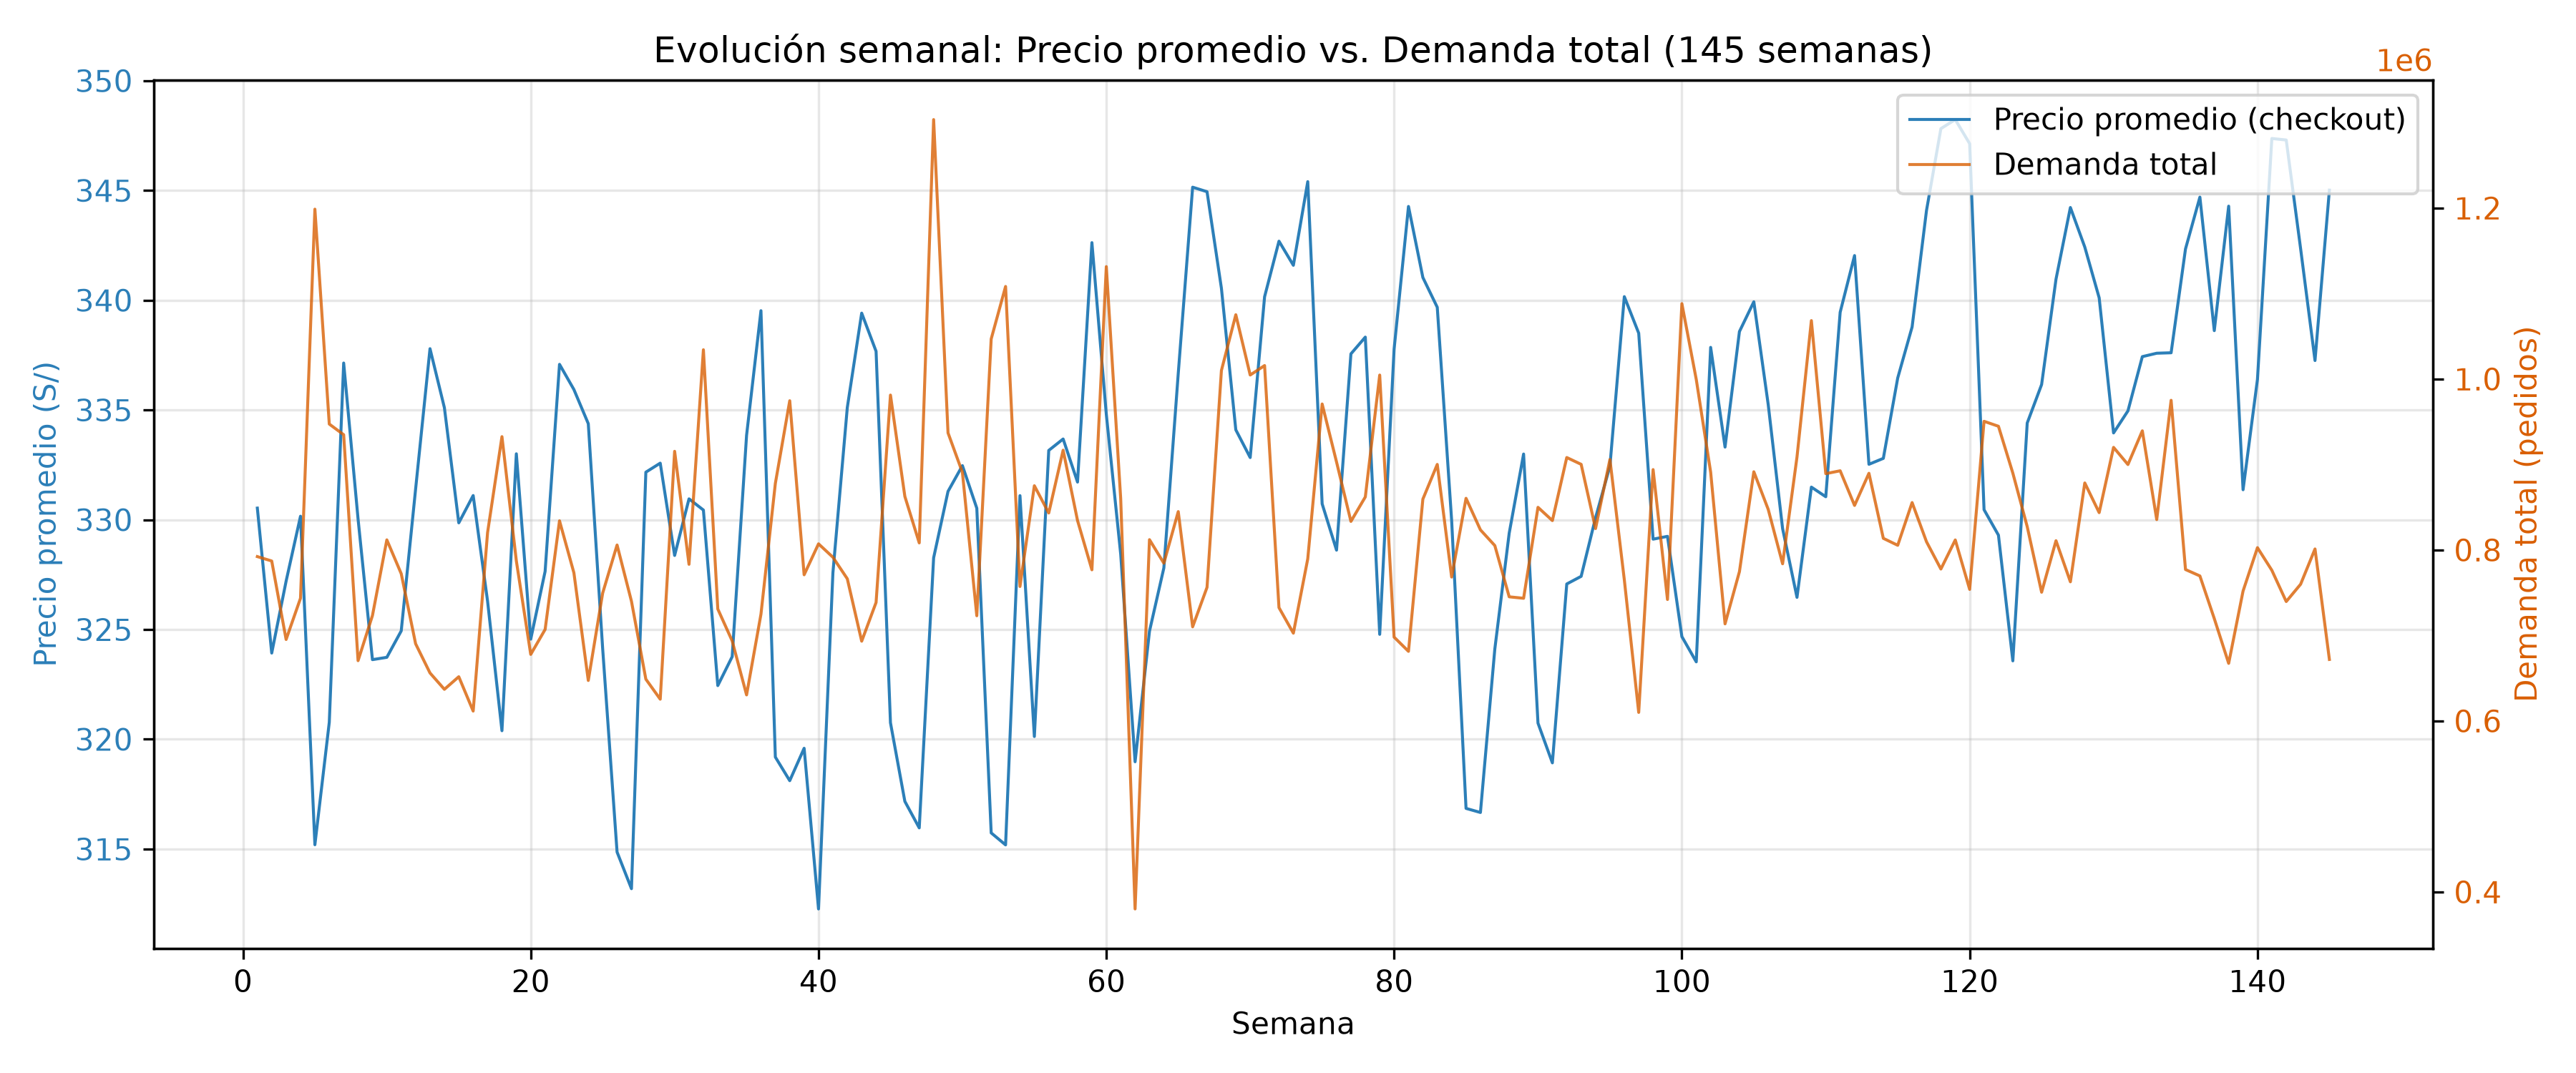
\includegraphics[width=0.85\textwidth]{figuras/evolucion_precio_demanda_semanal.png}
\caption{Evoluci\'on semanal del precio promedio de checkout y la demanda agregada (145 semanas). Muestra la din\'amica temporal conjunta de precio y cantidad.}
\label{fig:evolucion_precio_demanda}
\end{figure}

\begin{figure}[htbp]
\centering
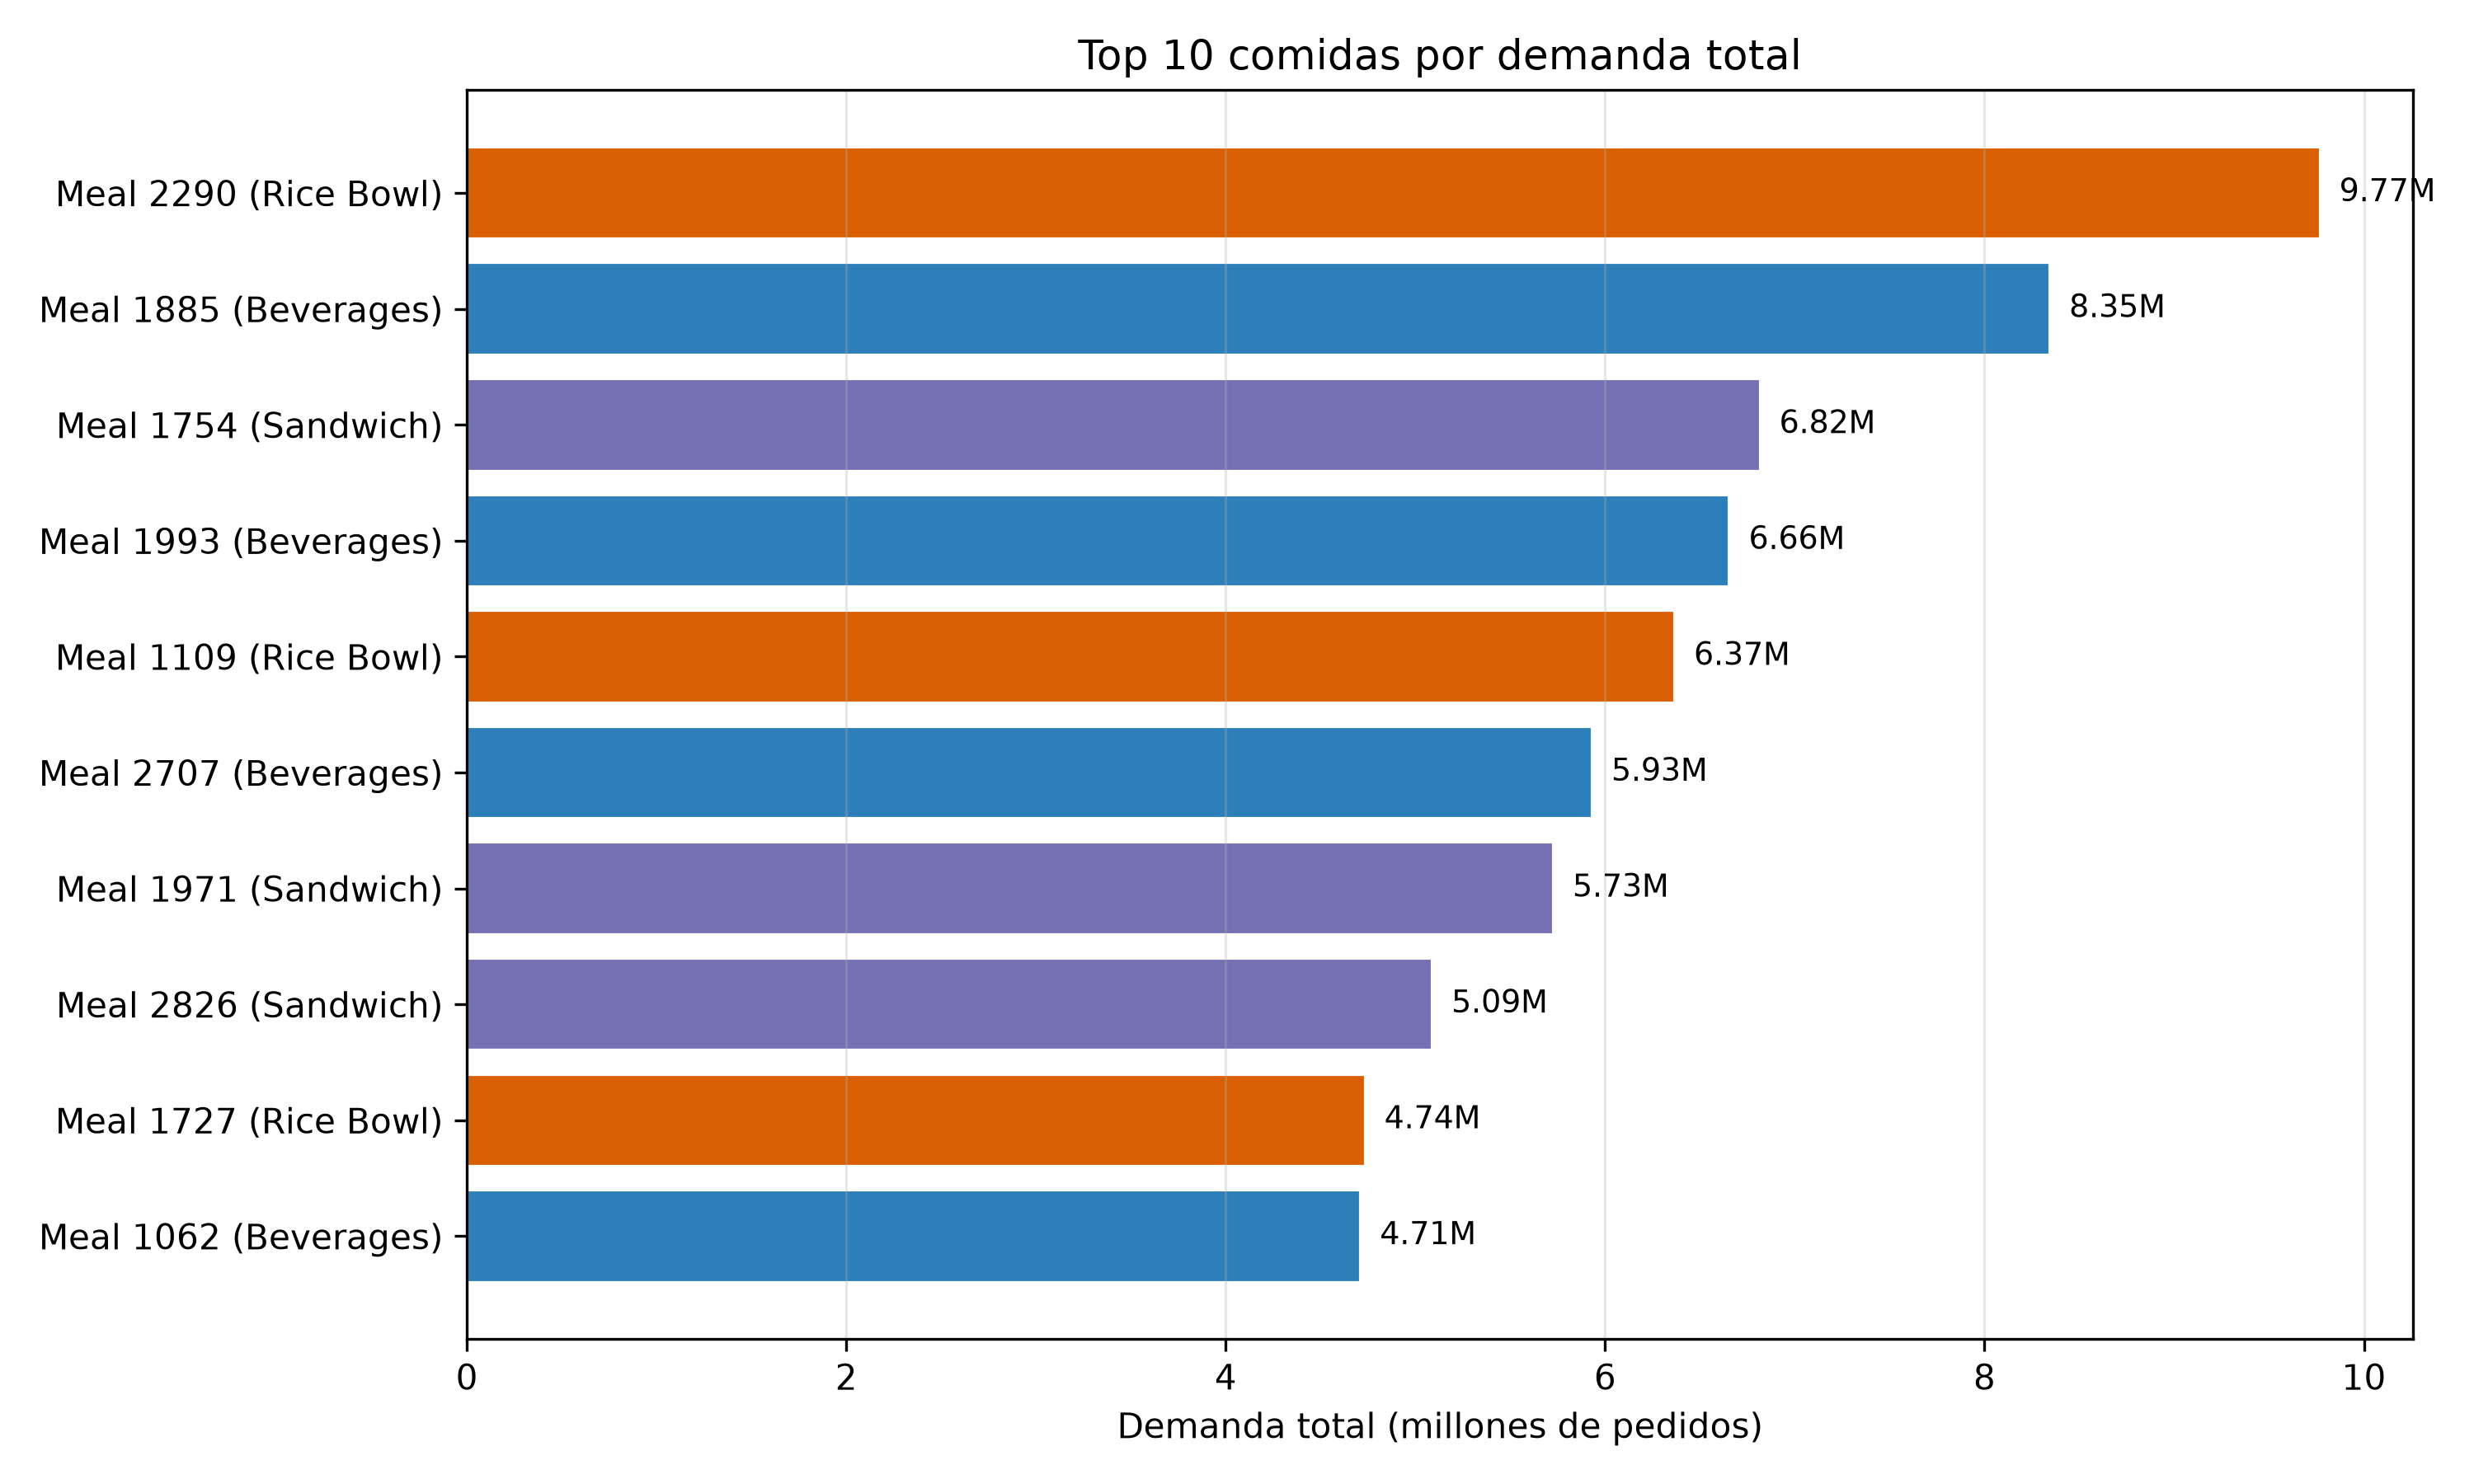
\includegraphics[width=0.85\textwidth]{figuras/top10_comidas_demanda.png}
\caption{Top 10 comidas por demanda total acumulada (145 semanas). Muestra la concentraci\'on de la demanda en pocos productos estrella.}
\label{fig:top10_comidas}
\end{figure}

\begin{figure}[htbp]
\centering
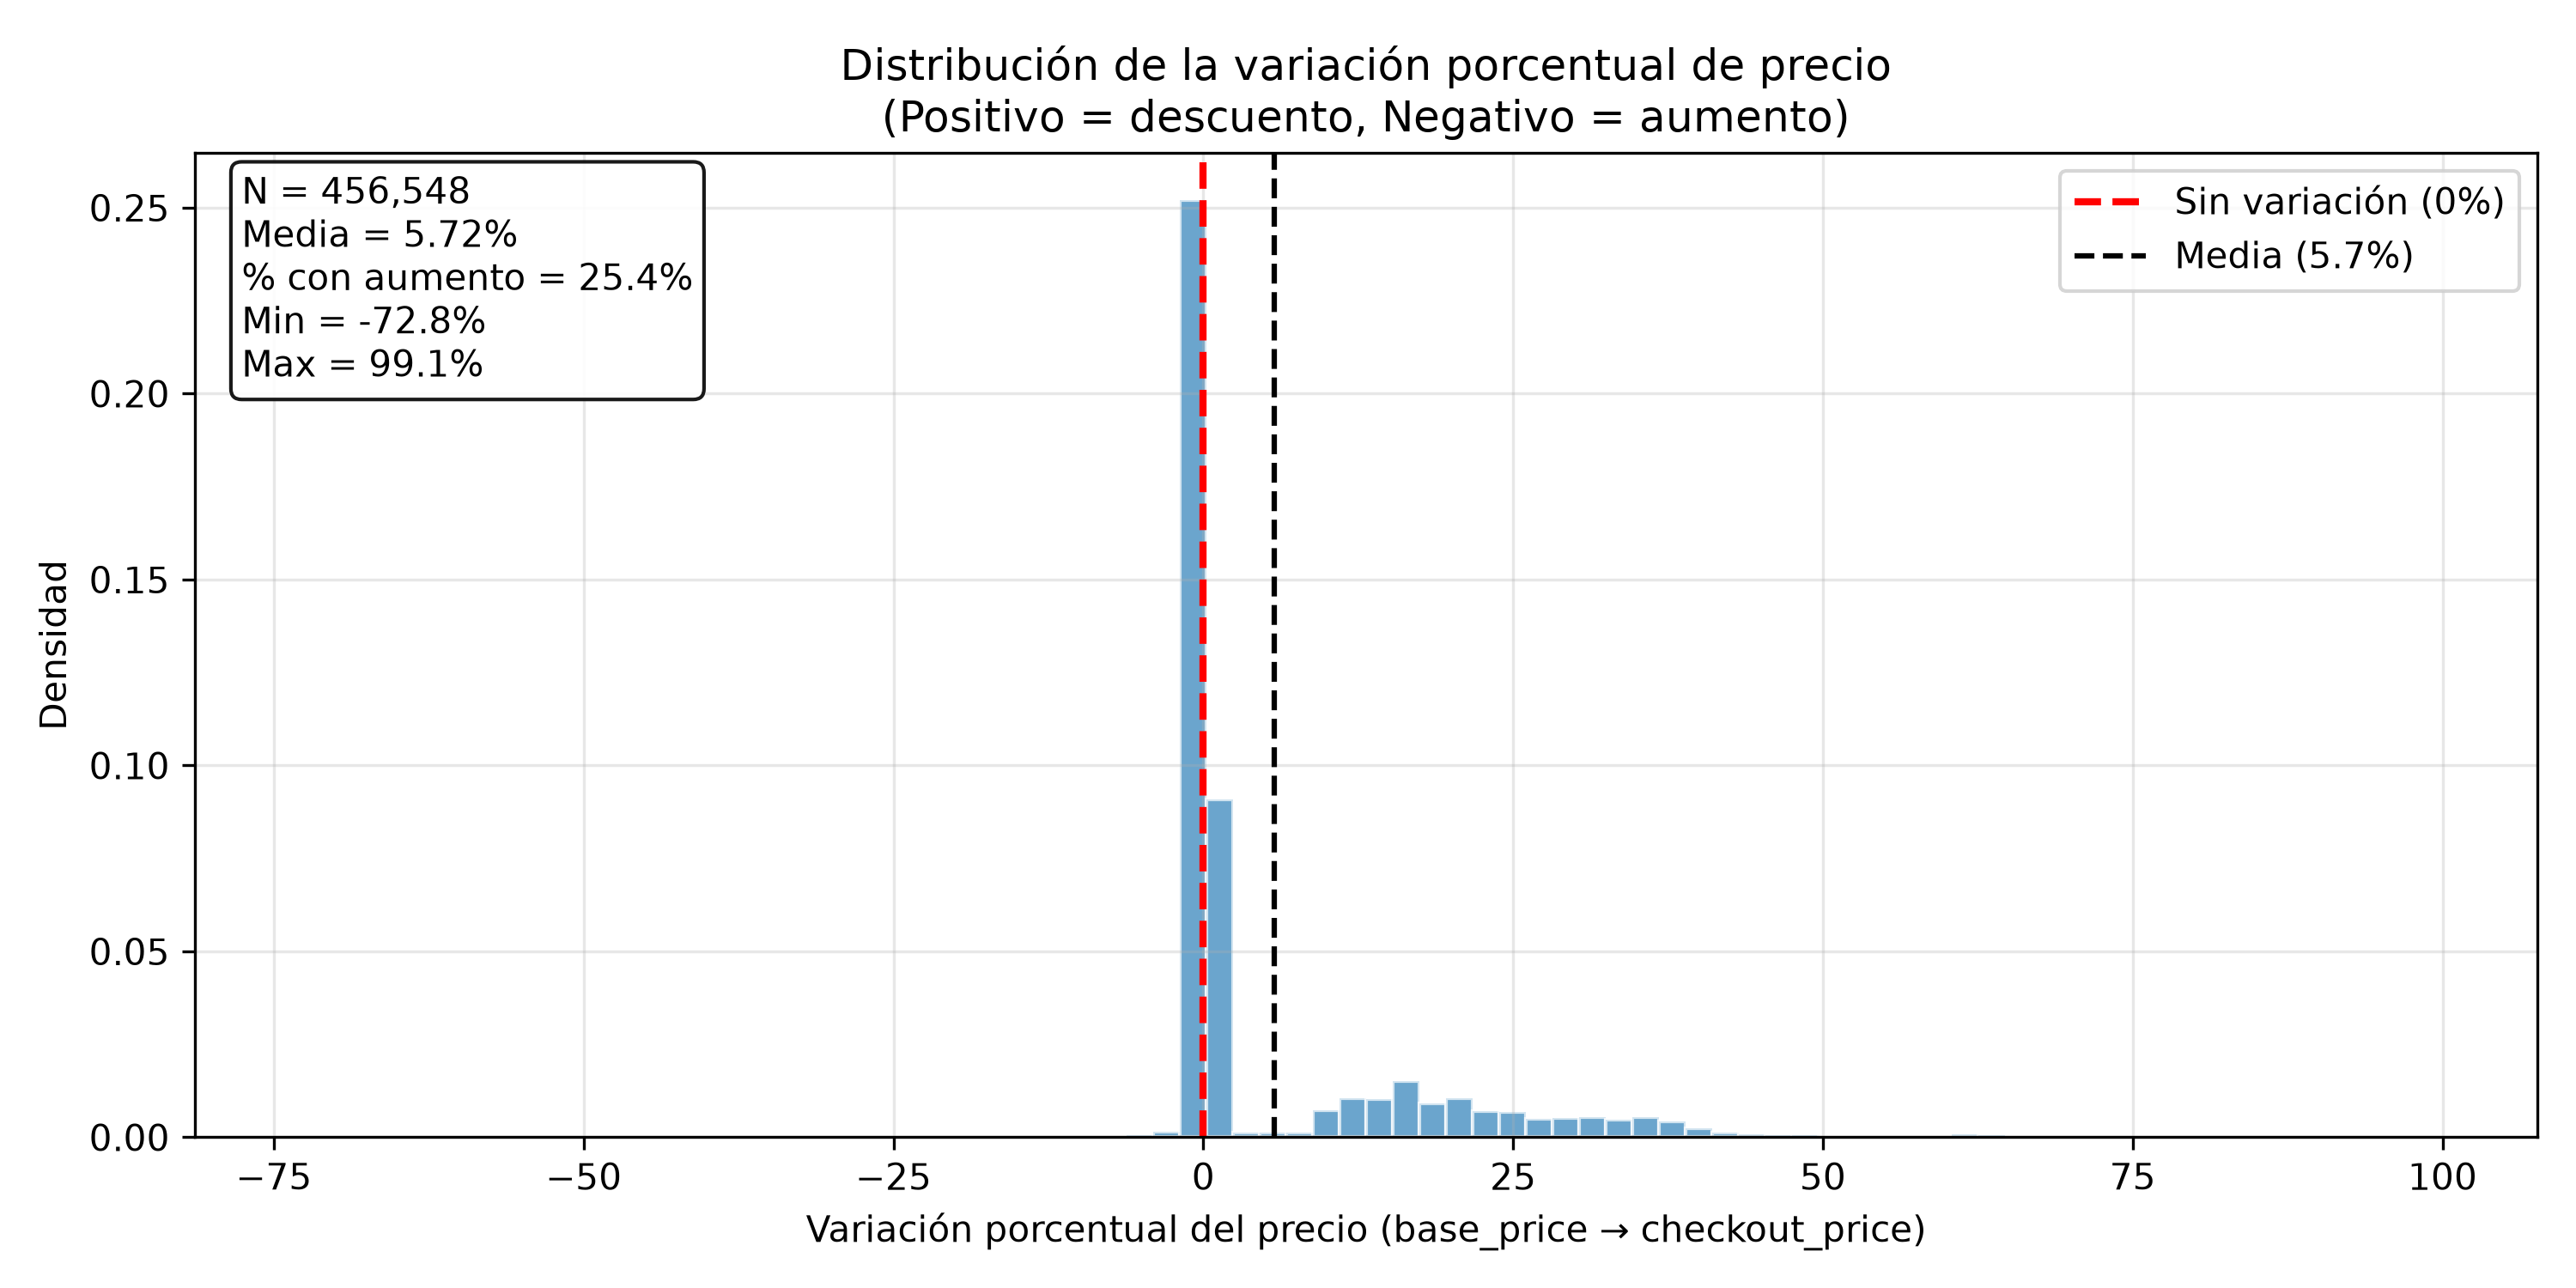
\includegraphics[width=0.85\textwidth]{figuras/histograma_variacion_precio_pct.png}
\caption{Distribuci\'on de la variaci\'on porcentual de precio (\texttt{base\_price} $\rightarrow$ \texttt{checkout\_price}). Positivo = descuento, Negativo = aumento. Media = 6.19\%, 25.43\% con aumento.}
\label{fig:hist_variacion_precio}
\end{figure}

% ============================================================
% 3. PREPARACIÓN Y LIMPIEZA
% ============================================================
\section{Preparaci\'on y Limpieza de Datos}
\phantomsection
\label{sec:preparacion}

El pipeline de preparaci\'on sigue tres etapas secuenciales, implementadas en Python (\texttt{src/data\_prep.py}) y dise\~nadas para ser totalmente reproducibles: (1) carga y uni\'on de tablas, (2) construcci\'on de variables derivadas de precio, (3) transformaciones logar\'itmicas para modelado. Cada etapa incluye aserciones de integridad.

\subsection{Carga y uni\'on de tablas}
\label{sec:merge}

Las tres tablas se leen desde CSV y se unen mediante \texttt{meal\_id} y \texttt{center\_id} con \textit{left join} usando \texttt{train} como tabla base:

\begin{verbatim}
train.merge(meal_info, on='meal_id', how='left') \
     .merge(centers, on='center_id', how='left')
\end{verbatim}

Se verifica que el n\'umero de filas se mantenga id\'entico al de \texttt{train} original (456,548), descartando duplicados en las tablas de referencia o p\'erdidas por claves no coincidentes. Tras el merge, no se detectan valores nulos en ninguna columna, confirmando que para cada combinaci\'on presente en \texttt{train} existe informaci\'on completa en \texttt{meal\_info} y \texttt{fulfilment\_center\_info}.

\subsection{Construcci\'on de variables de precio}
\label{sec:vars_precio}

La variable \texttt{base\_price} act\'ua como precio de referencia, no como un precio m\'inimo garantizado. Al calcular la diferencia \texttt{base\_price} $-$ \texttt{checkout\_price}, se esperaba encontrar \'unicamente valores positivos o cero (descuentos). Sin embargo, el hallazgo central de la limpieza fue que \textbf{en 25.43\% de las observaciones (116,101 de 456,548), \texttt{checkout\_price} super\'o a \texttt{base\_price}}, produciendo una variaci\'on negativa.

Este patr\'on se verific\'o exhaustivamente para descartar error de datos: (a) la magnitud de los valores negativos es variada y sustancial (decenas a cientos de unidades), no concentrada en montos fijos peque\~nos que sugerir\'ian un cargo por servicio; (b) la incidencia est\'a distribuida de forma pareja entre pr\'acticamente todos los centros (del orden de 1,700--1,900 casos por centro entre los principales), descartando un error localizado en una fuente espec\'ifica. La interpretaci\'on es que \texttt{base\_price} es un precio de lista actualizado con menor frecuencia, mientras que \texttt{checkout\_price} fluct\'ua semana a semana por din\'amicas de costos, oferta/demanda o decisiones comerciales no observadas.

\medskip
\noindent Se construyen tres variables derivadas:

\begin{itemize}
    \item \texttt{variacion\_precio} = \texttt{base\_price} $-$ \texttt{checkout\_price} (diferencia absoluta; positiva = descuento, negativa = aumento).
    \item \texttt{variacion\_precio\_pct} = (\texttt{variacion\_precio} / \texttt{base\_price}) $\times$ 100 (variaci\'on porcentual respecto a la referencia).
    \item \texttt{hubo\_aumento} = 1 si \texttt{variacion\_precio} $<$ 0, 0 en caso contrario (indicador binario de que el precio final super\'o la referencia).
\end{itemize}

La decisi\'on de \textbf{no excluir} las observaciones con \texttt{hubo\_aumento} = 1 es deliberada: excluir sistem\'aticamente los casos donde el precio subi\'o introducir\'ia sesgo de selecci\'on, dejando el modelo estimado solo sobre per\'iodos de baja de precio, lo cual no representa el comportamiento real del mercado. La variable \texttt{hubo\_aumento} se incluye como control candidato en las especificaciones del modelo (la secci\'on \nameref{sec:especificaciones-modelo}) para capturar cualquier efecto asim\'etrico de aumentos vs. descuentos.

\subsection{Transformaciones logar\'itmicas}
\label{sec:transformaciones_log}

Para la especificaci\'on log-log de elasticidad (la secci\'on \nameref{sec:especificaciones-modelo}), se crean las versiones logar\'itmicas de precio y cantidad:

\begin{itemize}
    \item \texttt{log\_checkout\_price} = $\ln(\texttt{checkout\_price})$
    \item \texttt{log\_num\_orders} = $\ln(1 + \texttt{num\_orders})$  \hfill (\texttt{log1p})
\end{itemize}

El uso de \texttt{log1p} (logaritmo de $1+x$) en lugar de $\ln(x)$ para \texttt{num\_orders} garantiza que la transformaci\'on est\'e definida para todos los valores (aunque el m\'inimo observado es 13, \texttt{log1p} es la pr\'actica est\'andar en variables de conteo y preserva la interpretabilidad de elasticidad para valores peque\~nos). La distribuci\'on de \texttt{log\_num\_orders} se aproxima considerablemente a una forma de campana, mitigando la heterocedasticidad y justificando estad\'isticamente ---no solo te\'oricamente--- la especificaci\'on log-log.

\subsection{Estad\'isticos descriptivos completos (tras preparaci\'on)}

\Cref{table:descriptivos_completa} presenta los estad\'isticos descriptivos de todas las variables num\'ericas relevantes despu\'es de la preparaci\'on, incluyendo las transformaciones logar\'itmicas y las variables de precio derivadas.

\begin{table}[htbp]
\centering
\caption{Estad\'isticos descriptivos completos tras preparaci\'on de datos.}
\label{table:descriptivos_completa}
\scriptsize
\setlength{\tabcolsep}{3pt}
\begin{threeparttable}
\begin{tabular}{@{}lrrrrrrr@{}}\toprule
Variable & Media & Desv. est. & M\'inimo & P25 & Mediana & P75 & M\'aximo \\\midrule
\texttt{checkout\_price} & 332.24 & 152.94 & 2.97 & 228.95 & 296.82 & 445.23 & 866.27 \\
\texttt{base\_price} & 354.16 & 160.72 & 55.35 & 243.50 & 310.46 & 458.87 & 866.27 \\
\texttt{num\_orders} & 261.87 & 395.92 & 13.00 & 54.00 & 136.00 & 324.00 & 24,299.00 \\
\texttt{variacion\_precio} & 21.92 & 48.50 & $-185.30$ & $-1.00$ & 1.00 & 16.52 & 561.60 \\
\texttt{variacion\_precio\_pct} & 6.19 & 13.65 & $-52.34$ & $-0.33$ & 0.32 & 5.31 & 100.00 \\
\texttt{hubo\_aumento} & 0.2543 & 0.435 & 0.00 & 0.00 & 0.00 & 1.00 & 1.00 \\
\texttt{log\_checkout\_price} & 5.65 & 0.48 & 1.09 & 5.43 & 5.69 & 6.10 & 6.76 \\
\texttt{log\_num\_orders} & 4.79 & 1.20 & 2.64 & 4.01 & 4.92 & 5.79 & 10.10 \\
\texttt{emailer\_for\_promotion} & 0.042 & 0.201 & 0.00 & 0.00 & 0.00 & 0.00 & 1.00 \\
\texttt{homepage\_featured} & 0.099 & 0.299 & 0.00 & 0.00 & 0.00 & 0.00 & 1.00 \\
\bottomrule
\end{tabular}
\begin{tablenotes}
\footnotesize
\item \textit{Nota.} $N = 456,548$. \texttt{hubo\_aumento}, \texttt{emailer\_for\_promotion} y \texttt{homepage\_featured} son binarias (0/1); su media reporta la proporci\'on de unos. \texttt{variacion\_precio\_pct} en puntos porcentuales.
\end{tablenotes}
\end{threeparttable}
\end{table}

Observaciones destacadas de \cref{table:descriptivos_completa}:

\begin{enumerate}
    \item La proporci\'on de observaciones con \texttt{hubo\_aumento} = 1 es 0.2543 (25.43\%), confirmando la magnitud del hallazgo.
    \item Las variables promocionales tienen prevalencia baja (\texttt{emailer\_for\_promotion}: 4.2\%; \texttt{homepage\_featured}: 9.9\%), t\'ipico de campa\~nas puntuales.
    \item \texttt{log\_num\_orders} tiene media 4.79 y desviaci\'on 1.20, con rango aproximado [2.64, 10.10], distribuci\'on sustancialmente m\'as sim\'etrica que la variable original.
    \item \texttt{variacion\_precio\_pct} tiene media positiva (6.19\%), indicando que en promedio el precio final est\'a por debajo de la referencia, pero con cola izquierda que llega a $-52.34$\% (aumentos sustanciales respecto al precio base).
\end{enumerate}

El \textit{DataFrame} final resultante (\texttt{demanda\_limpia.csv}) contiene 456,548 filas y 23 columnas (20 originales + 3 derivadas), listo para la etapa de modelado descrita a continuaci\'on.

\begin{figure}[htbp]
\centering
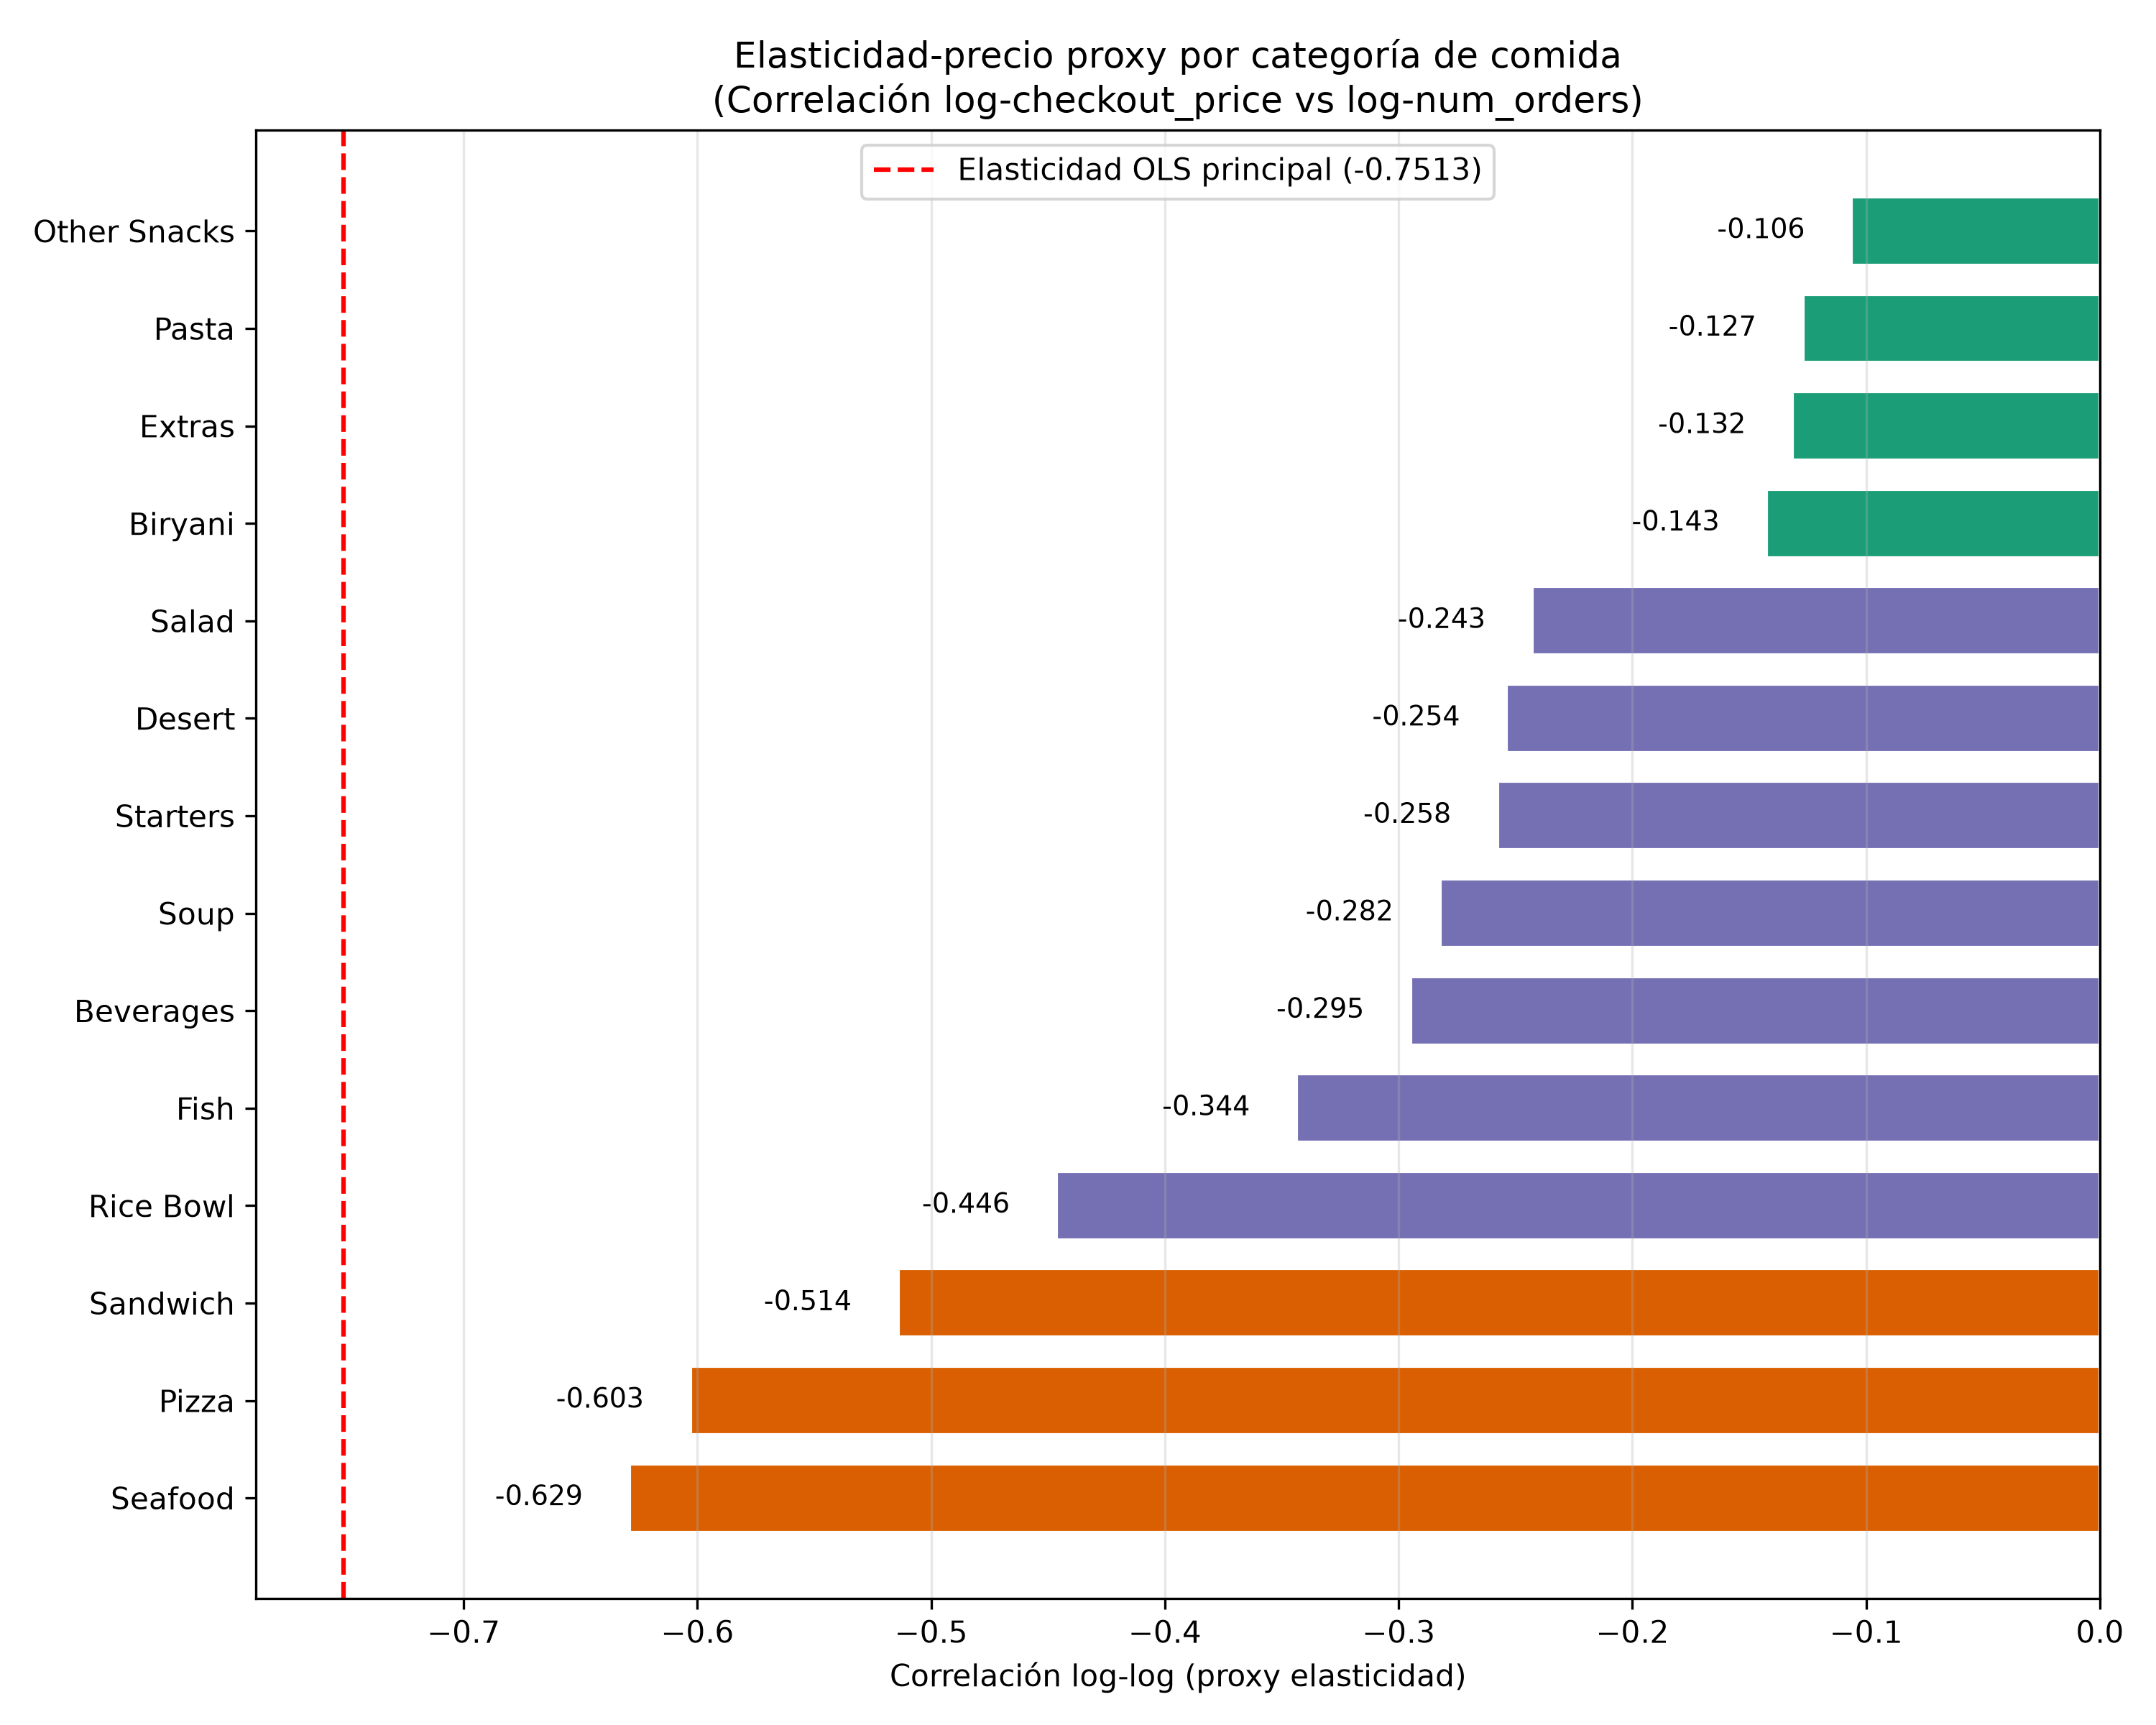
\includegraphics[width=0.85\textwidth]{figuras/elasticidad_por_categoria.png}
\caption{Elasticidad-precio proxy por categor\'ia de comida (Correlaci\'on log-log entre \texttt{checkout\_price} y \texttt{num\_orders}). L\'inea roja: elasticidad OLS principal (-0.7513).}
\label{fig:elasticidad_por_categoria}
\end{figure}

\begin{figure}[htbp]
\centering
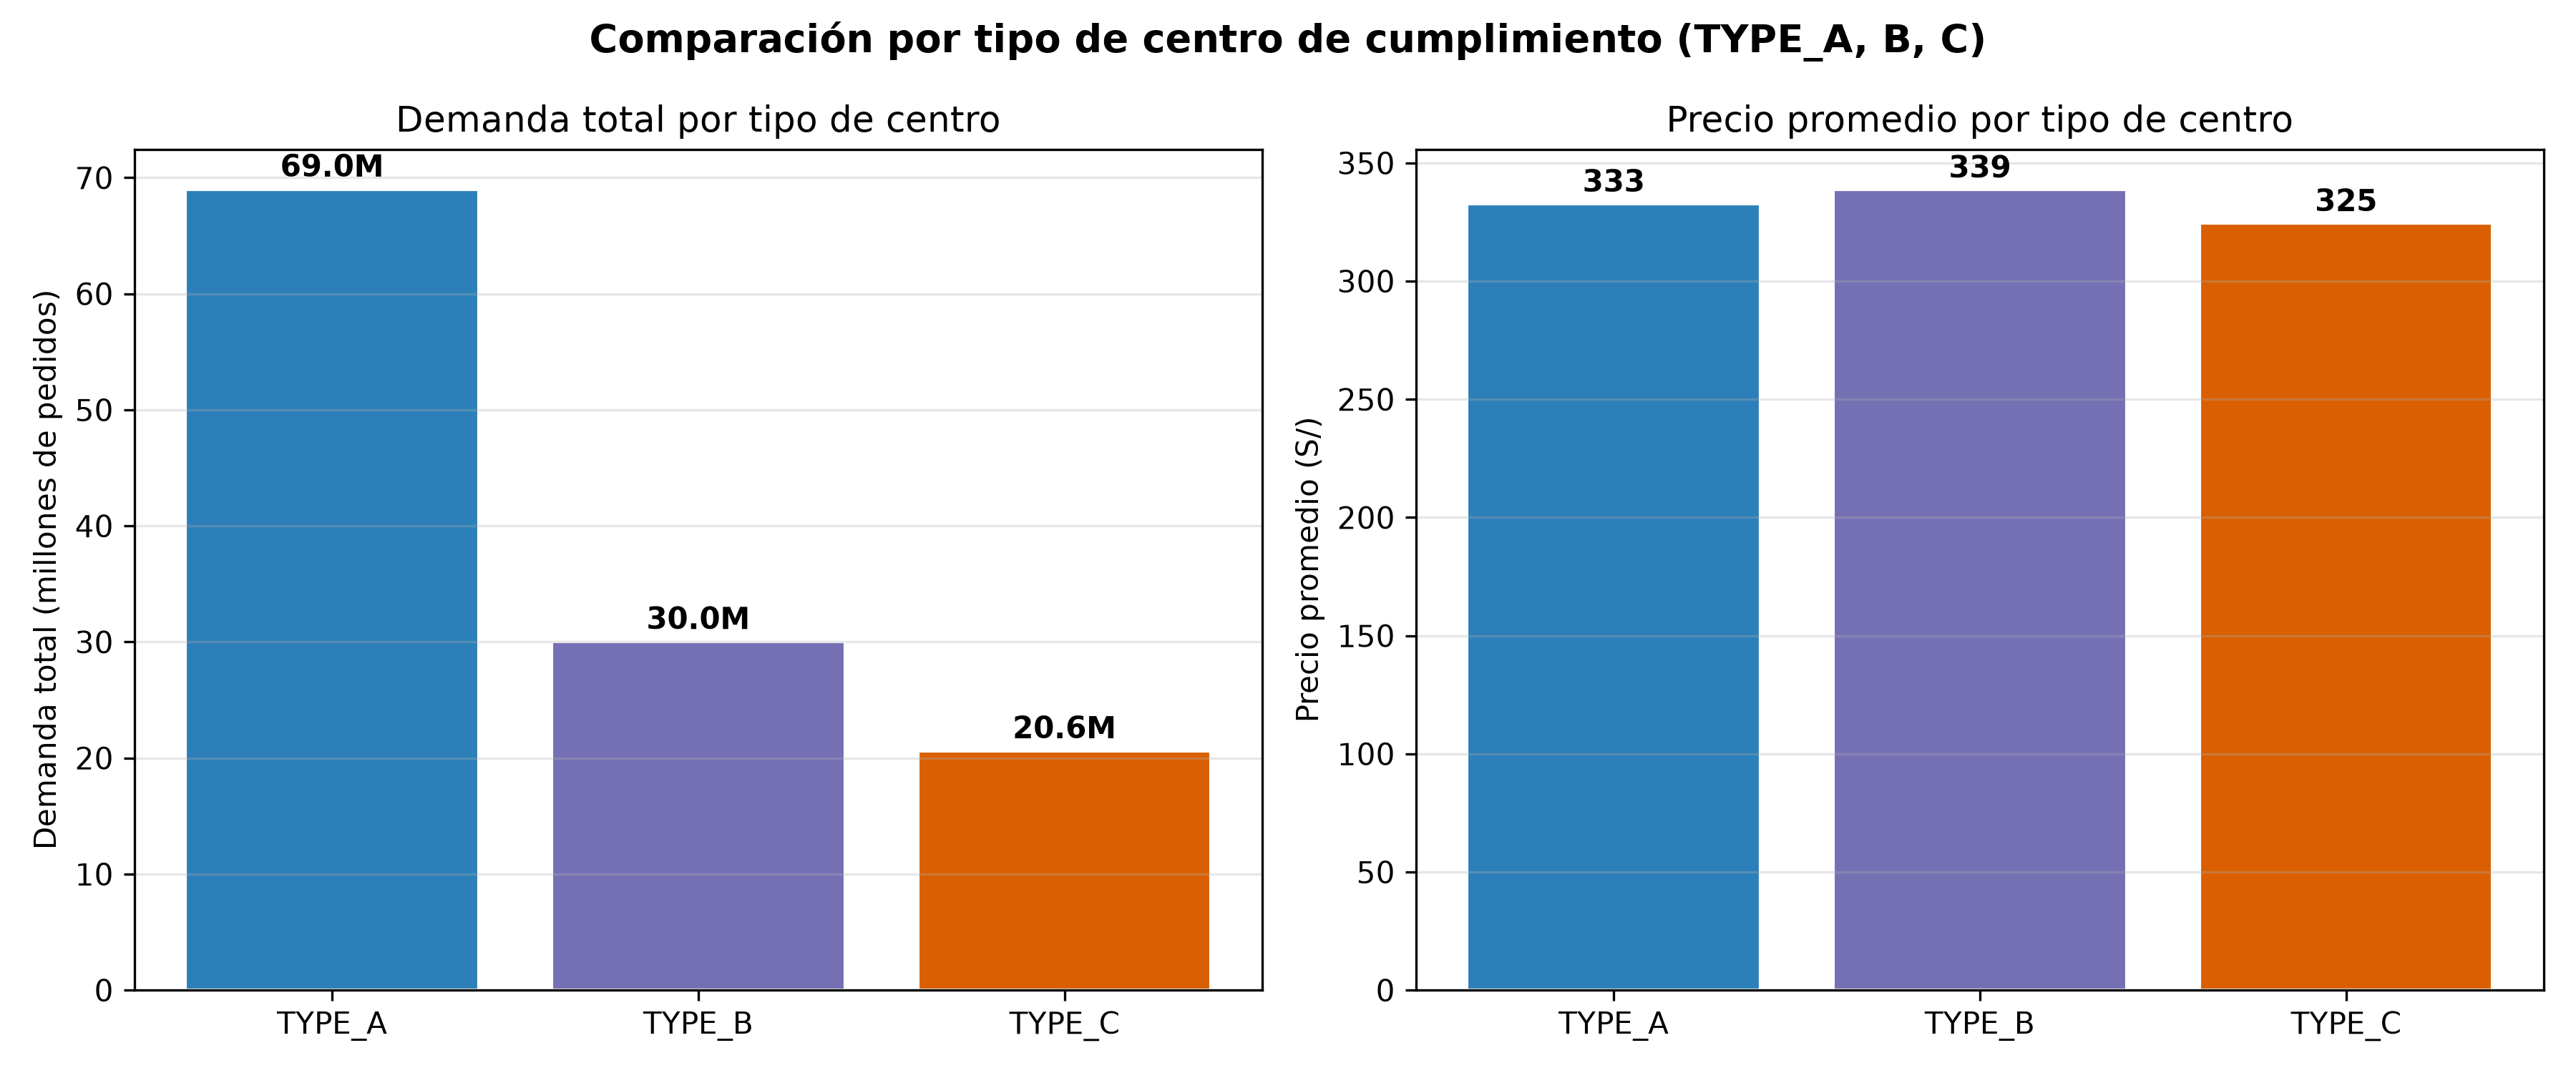
\includegraphics[width=0.85\textwidth]{figuras/comparacion_tipo_centro.png}
\caption{Comparaci\'on de demanda promedio por tipo de centro (TYPE\_A, TYPE\_B, TYPE\_C). TYPE\_B muestra mayor demanda relativa; TYPE\_C, menor.}
\label{fig:comparacion_tipo_centro}
\end{figure}

\begin{figure}[htbp]
\centering
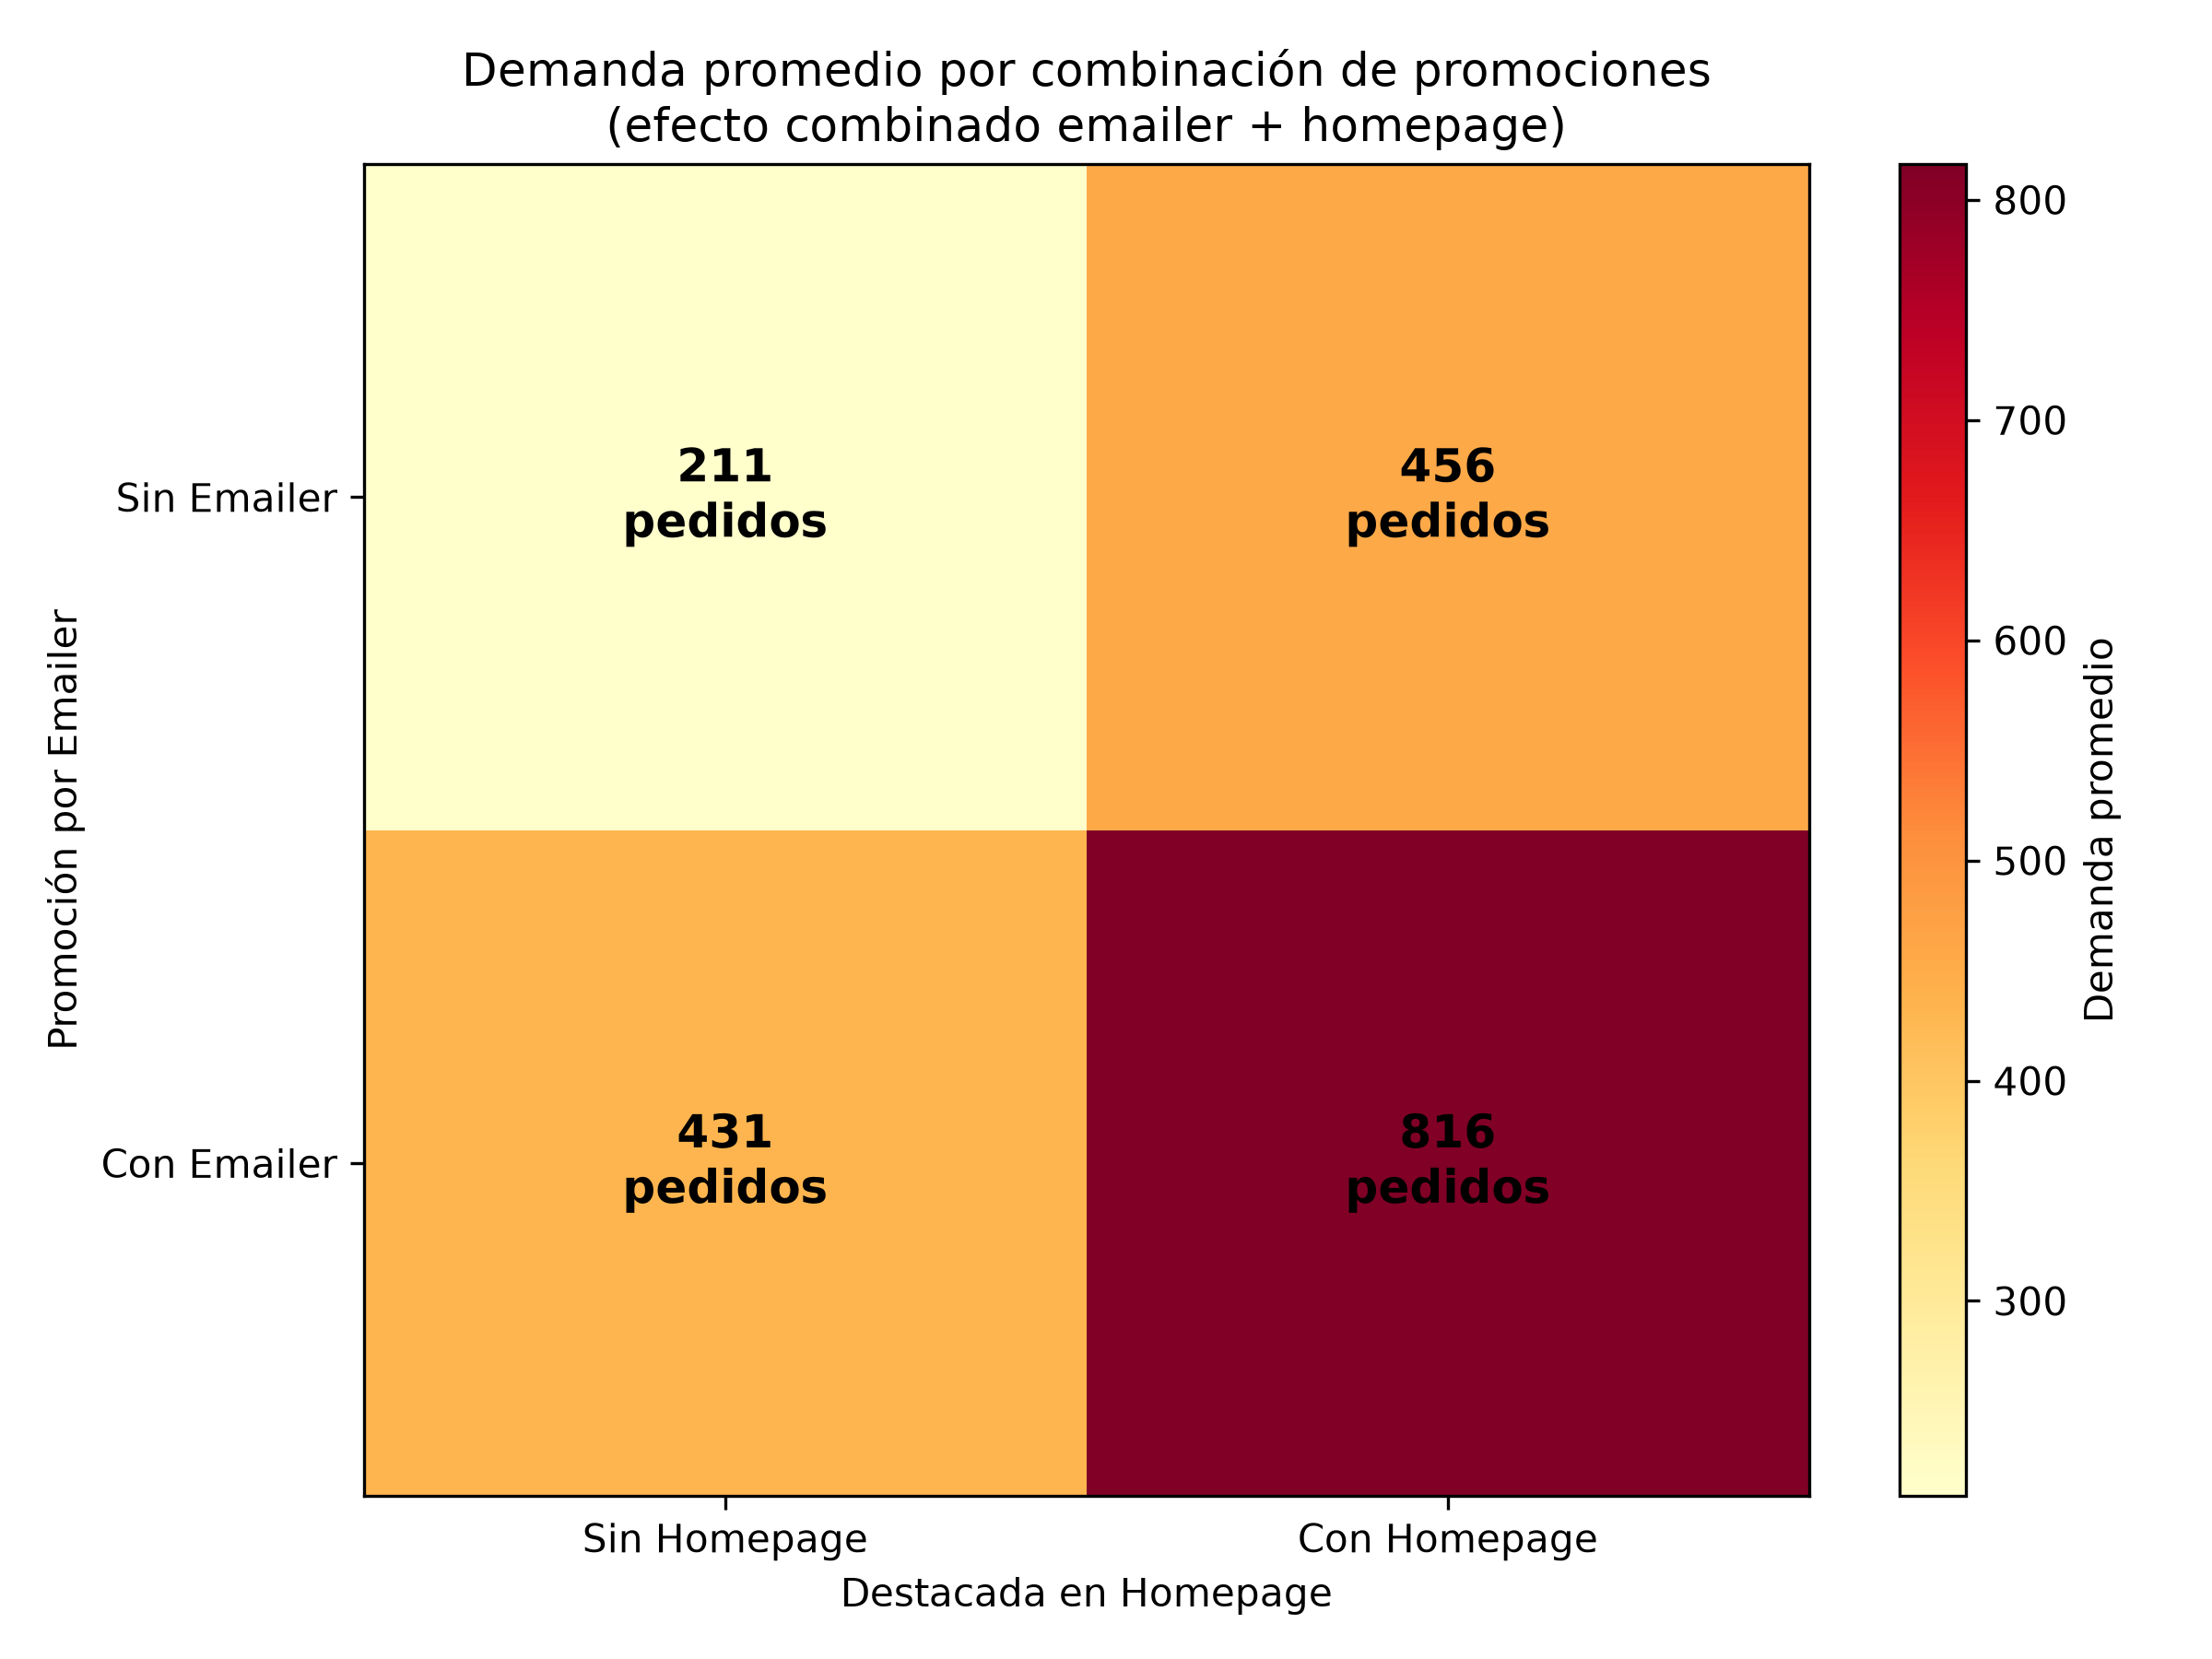
\includegraphics[width=0.85\textwidth]{figuras/efecto_promociones_matriz.png}
\caption{Matriz de efectos promocionales: demanda promedio por combinaci\'on de \texttt{emailer\_for\_promotion} y \texttt{homepage\_featured}. La exposici\'on en homepage tiene mayor impacto marginal que el emailer.}
\label{fig:efecto_promociones_matriz}
\end{figure}

% ============================================================
% 4. MARCO METODOLÓGICO
% ============================================================
\section{Marco Metodol\'ogico}
\label{sec:marco-metodologico}

El presente estudio adopta un enfoque econom\'etrico basado en \textbf{m\'inimos cuadrados ordinarios (OLS)} sobre una especificaci\'on \textbf{log-log} para estimar la elasticidad precio de la demanda en un servicio de \textit{food delivery}. La variable dependiente es el logaritmo natural del n\'umero de \'ordenes (\texttt{log\_num\_orders}) y la variable explicativa principal es el logaritmo natural del precio de checkout (\texttt{log\_checkout\_price}).

\begin{equation}
\log(\text{num\_orders}_i) = \beta_0 + \beta_1 \log(\text{checkout\_price}_i) + \varepsilon_i
\label{eq:modelo-base}
\end{equation}

La elecci\'on de la especificaci\'on log-log obedece a su interpretaci\'on directa: el coeficiente $\beta_1$ representa la \textbf{elasticidad precio de la demanda}, es decir, el cambio porcentual en la cantidad demandada asociado a un cambio del 1\% en el precio. Una elasticidad negativa indica que la demanda responde inversamente al precio (ley de la demanda), mientras que su magnitud informa sobre la sensibilidad de los consumidores.

\subsection{Justificaci\'on de variables de control}

Para mitigar sesgos de variable omitida y aislar el efecto asociado del precio sobre la demanda, se incorporan controles que capturan factores de oferta y demanda observables:

\begin{itemize}
    \item \texttt{emailer\_for\_promotion} (binaria): indica si la comida fue promocionada por correo electr\'onico. Las promociones aumentan la visibilidad y pueden desplazar la curva de demanda.
    \item \texttt{homepage\_featured} (binaria): indica si la comida apareci\'o destacada en la p\'agina principal. Al igual que el correo, afecta la exposici\'on del producto.
    \item \texttt{hubo\_aumento} (binaria): igual a 1 si el precio de checkout supera el precio base de referencia. Captura posibles efectos de \textit{reference pricing} y aversi\'on a p\'erdidas \parencite{kahneman1991}.
    \item \texttt{C(category)}: efectos fijos por categor\'ia de comida (13 categor\'ias). Controla preferencias sistem\'aticas por tipo de comida.
    \item \texttt{C(center\_type)}: efectos fijos por tipo de centro de cumplimiento (TYPE\_A, TYPE\_B, TYPE\_C). Captura heterogeneidad operativa y geogr\'afica no observada.
\end{itemize}

El dataset procesado contiene $N = 456,548$ observaciones a nivel de comida-semana-centro, lo que confiere alta potencia estad\'istica para detectar efectos incluso de magnitud peque\~na.

\subsection{Especificaciones del modelo}
\label{sec:especificaciones-modelo}

Se estiman tres especificaciones anidadas para evaluar robustez y comparar ajustes mediante criterios de informaci\'on (AIC, BIC) y $R^2$ ajustado.

\subsubsection{Modelo 1: especificaci\'on base (log-log simple)}
\begin{equation}
\log(\text{num\_orders}_i) = \beta_0 + \beta_1 \log(\text{checkout\_price}_i) + \varepsilon_i
\label{eq:modelo-1}
\end{equation}

\subsubsection{Modelo 2: log-log con controles (especificaci\'on principal)}
\begin{equation}
\begin{aligned}
\log(\text{num\_orders}_i) = \beta_0 &+ \beta_1 \log(\text{checkout\_price}_i) \\
&+ \beta_2 \text{emailer\_for\_promotion}_i + \beta_3 \text{homepage\_featured}_i \\
&+ \beta_4 \text{hubo\_aumento}_i \\
&+ \sum_{k=1}^{13} \gamma_k \mathbb{1}[\text{category}_i = k] \\
&+ \sum_{m=1}^{2} \delta_m \mathbb{1}[\text{center\_type}_i = m] + \varepsilon_i
\end{aligned}
\label{eq:modelo-2}
\end{equation}

\subsubsection{Modelo 3: semi-log con controles (especificaci\'on alternativa)}
\begin{equation}
\begin{aligned}
\log(\text{num\_orders}_i) = \beta_0 &+ \beta_1 \text{checkout\_price}_i \\
&+ \beta_2 \text{emailer\_for\_promotion}_i + \beta_3 \text{homepage\_featured}_i \\
&+ \beta_4 \text{hubo\_aumento}_i \\
&+ \sum_{k=1}^{13} \gamma_k \mathbb{1}[\text{category}_i = k] \\
&+ \sum_{m=1}^{2} \delta_m \mathbb{1}[\text{center\_type}_i = m] + \varepsilon_i
\end{aligned}
\label{eq:modelo-3}
\end{equation}

En el Modelo 3, el coeficiente $\beta_1$ se interpreta como \textit{semi-elasticidad}: el cambio porcentual en la demanda por cada unidad monetaria de aumento en el precio (no elasticidad constante). \Cref{tab:variables-modelos} resume las variables incluidas en cada especificaci\'on; los criterios de ajuste (AIC, BIC, $R^2$) se reportan y comparan en la secci\'on \nameref{subsec:comparacion_modelos}, junto con los resultados.

\begin{table}[htbp]
\centering
\caption{Variables incluidas en cada especificaci\'on del modelo.}
\label{tab:variables-modelos}
\begin{tabular}{lccc}
\toprule
\textbf{Variable} & \textbf{Modelo 1} & \textbf{Modelo 2} & \textbf{Modelo 3} \\
\midrule
$\log(\text{checkout\_price})$ & \checkmark & \checkmark & -- \\
$\text{checkout\_price}$ (nivel) & -- & -- & \checkmark \\
$\text{emailer\_for\_promotion}$ & -- & \checkmark & \checkmark \\
$\text{homepage\_featured}$ & -- & \checkmark & \checkmark \\
$\text{hubo\_aumento}$ & -- & \checkmark & \checkmark \\
$\text{C(category)}$ (13 dummies) & -- & \checkmark & \checkmark \\
$\text{C(center\_type)}$ (2 dummies) & -- & \checkmark & \checkmark \\
\bottomrule
\end{tabular}
\end{table}

\subsection{Validaci\'on de supuestos: procedimiento}
\label{sec:validacion-supuestos}

La validez inferencial de OLS requiere verificar los supuestos cl\'asicos. Los resultados num\'ericos de cada test se reportan en la secci\'on \nameref{sec:validacion} (heterocedasticidad, multicolinealidad, normalidad y autocorrelaci\'on); aqu\'i se documenta el procedimiento y la decisi\'on asociada a cada uno.

\begin{itemize}
    \item \textbf{Heterocedasticidad (Breusch-Pagan)}: $H_0$: varianza de los errores constante vs. $H_1$: varianza funci\'on de los regresores. De rechazarse $H_0$, se reportan errores est\'andar robustos \textbf{HC3}, v\'alidos asint\'oticamente en muestras grandes \parencite{davidson1994stochastic} y preferibles a HC0/HC1 cuando existe apalancamiento en los datos \parencite{long2000heteroscedasticity}.
    \item \textbf{Multicolinealidad (VIF)}: calculado sobre las variables num\'ericas continuas del modelo (\texttt{log\_checkout\_price}, \texttt{emailer\_for\_promotion}, \texttt{homepage\_featured}, \texttt{hubo\_aumento}). Las dummies de efectos fijos se excluyen del c\'alculo porque su VIF individual dentro de un conjunto mutuamente excluyente no tiene interpretaci\'on est\'andar.
    \item \textbf{Normalidad de residuos (Jarque-Bera y Q-Q plot)}: $H_0$: residuos $\sim \mathcal{N}(0,\sigma^2)$. Con $N=456,548$ se anticipa que la prueba tenga potencia excesiva y rechace desviaciones m\'inimas sin relevancia pr\'actica; por ello se complementa con inspecci\'on visual del gr\'afico Q-Q.
    \item \textbf{Autocorrelaci\'on (Durbin-Watson)}: valores cercanos a 2 indican ausencia de autocorrelaci\'on. Dada la estructura de panel (semana $\times$ centro $\times$ comida), es esperable cierta autocorrelaci\'on residual en ausencia de efectos fijos por semana.
\end{itemize}

\subsection{Intervalos de confianza por bootstrap: procedimiento}
\phantomsection
\label{sec:bootstrap}

Para obtener intervalos de confianza que no dependan de asunciones de normalidad ni de la estructura de covarianza anal\'itica, se implementa un \textbf{bootstrap no param\'etrico por remuestreo con reemplazo} sobre el modelo base (\cref{eq:modelo-1}).

\begin{enumerate}
    \item \textbf{Iteraciones}: $B = 1,000$ remuestras bootstrap.
    \item \textbf{Esquema de remuestreo}: muestreo con reemplazo de tama\~no $n = N = 456,548$, preservando la distribuci\'on emp\'irica conjunta de todas las variables.
    \item \textbf{Estimaci\'on por iteraci\'on}: en cada remuestra $b = 1,\dots,B$, se ajusta el modelo base y se almacena el coeficiente $\hat{\beta}_1^{(b)}$.
    \item \textbf{Intervalo de confianza}: percentil 2.5 y 97.5 de la distribuci\'on emp\'irica $\{\hat{\beta}_1^{(b)}\}_{b=1}^B$.
    \item \textbf{Reproducibilidad}: semilla fija \texttt{seed = 42} (\texttt{numpy.random.default\_rng}).
\end{enumerate}

El bootstrap se realiz\'o sobre el modelo base por simplicidad computacional; los resultados num\'ericos se reportan en la secci\'on \nameref{sec:bootstrap_resultados}.

% ============================================================
% 5. RESULTADOS
% ============================================================
\section{Resultados Principales}
\label{sec:resultados}

\subsection{Comparaci\'on de modelos}
\label{subsec:comparacion_modelos}

\Cref{tab:comparacion_modelos} presenta los criterios de informaci\'on y bondad de ajuste de las tres especificaciones descritas en la secci\'on \nameref{sec:especificaciones-modelo}.

\begin{table}[htbp]
\centering
\caption{Comparaci\'on de modelos alternativos: criterios de informaci\'on y bondad de ajuste.}
\label{tab:comparacion_modelos}
\begin{tabular}{lcccc}
\toprule
Modelo & AIC & BIC & $R^2$ ajustado & $N$ \\
\midrule
Semi-log con controles & 1,112,317 & 1,112,537 & 0.5377 & 456,548 \\
Log-log con controles & 1,118,513 & 1,118,733 & 0.5314 & 456,548 \\
Log-log base & 1,394,427 & 1,394,449 & 0.1423 & 456,548 \\
\bottomrule
\end{tabular}
\end{table}

El modelo \textit{semi-log} con controles presenta el menor AIC y BIC, y el mayor $R^2$ ajustado (0.5377), indicando un mejor ajuste global. No obstante, el modelo \textit{log-log} con controles ofrece la ventaja de una interpretaci\'on directa de la elasticidad-precio como el coeficiente del logaritmo del precio, manteniendo un $R^2$ ajustado muy similar (0.5314). Dado el objetivo central de este trabajo —estimar la elasticidad-precio de la demanda—, se selecciona el modelo \textit{log-log} con controles como especificaci\'on principal.

\subsection{Modelo principal: log-log con controles}
\label{subsec:modelo_principal}

\Cref{tab:modelo_principal_completa} presenta los resultados completos del modelo \textit{log-log} con controles. Dada la estructura de panel de los datos (observaciones repetidas por combinaciones centro-comida a lo largo de 145 semanas), la inferencia principal utiliza \textbf{errores estándar clusterizados multiway por \texttt{center\_id} $\times$ \texttt{meal\_id}} (Cameron, Gelbach \& Miller, 2011), que permiten correlación arbitraria dentro de cada centro y dentro de cada comida. Los errores HC3 se reportan solo como referencia; no corrigen la autocorrelación intra-panel (Durbin-Watson $=1.195$).

\begin{table}[htbp]
\centering
\caption{Resultados completos del modelo log-log con controles (variable dependiente: $\log(\texttt{num\_orders})$). \textbf{Inferencia principal: multiway cluster \texttt{center\_id} $\times$ \texttt{meal\_id}}. HC3 solo referencia.}
\label{tab:modelo_principal_completa}
\begin{adjustwidth}{-1.2cm}{-1.2cm}
\centering
\footnotesize
\begin{tabular}{lcccccc}
\toprule
Variable & Coef. & SE Cl. & SE Multiway & $t$ (Multiway) & $p$ & IC 95\% (Multiway) \\
\midrule
Intercept & 9.0682 & 0.024 & 0.068 & 133.36 & <0.001 & [8.935, 9.201] \\
\texttt{C(category)[T.Biryani]} & $-$1.2347 & 0.007 & 0.019 & $-$64.98 & <0.001 & [$-$1.272, $-$1.197] \\
\texttt{C(category)[T.Desert]} & $-$0.6903 & 0.007 & 0.021 & $-$32.87 & <0.001 & [$-$0.731, $-$0.649] \\
\texttt{C(category)[T.Extras]} & 0.1599 & 0.007 & 0.022 & 7.27 & <0.001 & [0.117, 0.203] \\
\texttt{C(category)[T.Fish]} & $-$0.2589 & 0.010 & 0.031 & $-$8.35 & <0.001 & [$-$0.320, $-$0.198] \\
\texttt{C(category)[T.Other Snacks]} & $-$0.3560 & 0.005 & 0.017 & $-$20.94 & <0.001 & [$-$0.389, $-$0.323] \\
\texttt{C(category)[T.Pasta]} & $-$0.9255 & 0.006 & 0.019 & $-$48.71 & <0.001 & [$-$0.963, $-$0.888] \\
\texttt{C(category)[T.Pizza]} & 0.4756 & 0.007 & 0.023 & 20.68 & <0.001 & [0.431, 0.521] \\
\texttt{C(category)[T.Rice Bowl]} & 1.2474 & 0.006 & 0.018 & 69.30 & <0.001 & [1.212, 1.283] \\
\texttt{C(category)[T.Salad]} & 0.8328 & 0.006 & 0.017 & 48.99 & <0.001 & [0.799, 0.866] \\
\texttt{C(category)[T.Sandwich]} & 0.9604 & 0.005 & 0.017 & 56.49 & <0.001 & [0.927, 0.994] \\
\texttt{C(category)[T.Seafood]} & $-$0.3467 & 0.008 & 0.025 & $-$13.87 & <0.001 & [$-$0.396, $-$0.298] \\
\texttt{C(category)[T.Soup]} & $-$0.9220 & 0.008 & 0.024 & $-$38.42 & <0.001 & [$-$0.969, $-$0.875] \\
\texttt{C(category)[T.Starters]} & $-$0.2286 & 0.006 & 0.018 & $-$12.70 & <0.001 & [$-$0.264, $-$0.193] \\
\texttt{C(center\_type)[T.TYPE\_B]} & 0.2807 & 0.003 & 0.011 & 25.52 & <0.001 & [0.259, 0.302] \\
\texttt{C(center\_type)[T.TYPE\_C]} & $-$0.3526 & 0.003 & 0.011 & $-$32.05 & <0.001 [$-$0.374, $-$0.331] \\
\texttt{log\_checkout\_price} & \textbf{$-$0.7513} & 0.005 & \textbf{0.043} & $-$17.47 & <0.001 & \textbf{[$-$0.835, $-$0.667]} \\
\texttt{emailer\_for\_promotion} & 0.5028 & 0.005 & 0.016 & 31.43 & <0.001 & [0.471, 0.534] \\
\texttt{homepage\_featured} & 0.6492 & 0.004 & 0.015 & 43.28 & <0.001 & [0.619, 0.679] \\
\texttt{hubo\_aumento} & $-$0.0024 & 0.003 & 0.009 & $-$0.27 & 0.787 & [$-$0.020, 0.015] \\
\bottomrule
\end{tabular}
\end{adjustwidth}
\end{table}

\textbf{Nota:} Los errores estándar multiway son $\approx 8\times$ mayores que los HC3 para \texttt{log\_checkout\_price} (0.043 vs 0.005), reflejando la dependencia intra-panel no capturada por HC3. El IC 95\% multiway $[-0.835, -0.667]$ es la inferencia principal; el IC HC3 $[-0.762, -0.741]$ subestima severamente la incertidumbre.

\textbf{Interpretaci\'on de la proyecci\'on log-log promedio.} El coeficiente de \texttt{log\_checkout\_price} en la especificaci\'on log-log con controles es $-0.7513$. La inferencia principal usa \textbf{errores estándar multiway cluster \texttt{center\_id} $\times$ \texttt{meal\_id}} (SE = 0.043, IC 95\% $[-0.835, -0.667]$), coherentes con la estructura de panel; los SE HC3 (0.005, IC $[-0.762, -0.741]$) subestiman la incertidumbre al ignorar la autocorrelación intra-panel (DW $=1.195$). Esto implica que un aumento del 1\% en el precio de checkout se asocia con una disminuci\'on promedio del 0.7513\% en el n\'umero de \'ordenes, \textit{ceteris paribus}, \emph{bajo la imposición de una elasticidad constante}. La demanda resulta inel\'astica en promedio ($|\eta| < 1$), consistente con la literatura FAFH. \textbf{Advertencia:} los tests RESET ($F=119.57$, $p\approx0$) y RCS (Wald $\chi^2(3)=10\,279$, $p\approx0$) rechazan rotundamente la linealidad log-log; la elasticidad real varía con el precio ($+0.58$ a $-3.22$ seg\'un RCS). Este valor es una \emph{proyección promedio}, no una elasticidad estructural constante.

\textbf{Comparaci\'on con modelos alternativos.} \Cref{tab:comparacion_elasticidades} contrasta la elasticidad del modelo principal con las especificaciones alternativas.

\begin{table}[htbp]
\centering
\caption{Comparaci\'on de elasticidades-precio entre especificaciones.}
\label{tab:comparacion_elasticidades}
\begin{tabular}{lcc}
\toprule
Especificaci\'on & Elasticidad & Nota \\
\midrule
Log-log base (sin controles) & $-$0.9398 & Sesgo por variable omitida \\
Semi-log con controles (eval. en media) & $-$1.0624 & $\hat{\beta}_{\text{price}} \times \bar{P} = -0.0032 \times 332.24$ \\
Log-log con controles (principal) & \textbf{$-$0.7513} & \textbf{Proyección promedio; IC 95\% multiway $[-0.835,-0.667]$} \\
\bottomrule
\end{tabular}
\end{table}

El modelo base sobreestima la elasticidad en magnitud ($-0.9398$ vs. $-0.7513$), sugiriendo sesgo por variable omitida al no controlar por categor\'ia, tipo de centro y promociones. El modelo \textit{semi-log} evaluado en la media del precio ($332.24$) produce una elasticidad equivalente de $-1.0624$, considerablemente m\'as el\'astica. La diferencia radica en la forma funcional: el modelo \textit{semi-log} impone una elasticidad que var\'ia con el nivel de precio ($\eta = \beta \times P$), mientras que el \textit{log-log} asume elasticidad constante. La elecci\'on del \textit{log-log} se justifica por su interpretabilidad directa y por ser la especificaci\'on est\'andar en la literatura de demanda de alimentos preparados.

\subsection{Validaci\'on de supuestos: resultados}
\label{sec:validacion}

Esta secci\'on reporta los resultados num\'ericos de los tests descritos en la secci\'on \nameref{sec:validacion-supuestos}, aplicados a la especificaci\'on principal (\textit{log-log} con controles).

\subsubsection{Heterocedasticidad}
\label{subsec:heterocedasticidad}

\begin{table}[htbp]
\centering
\caption{Prueba de Breusch-Pagan para heterocedasticidad.}
\label{tab:breusch_pagan}
\begin{tabular}{lcc}
\toprule
Estad\'istico & Valor & $p$-valor \\
\midrule
Lagrange Multiplier (LM) & 34,632.47 & <0.001 \\
$F$ & 1,972.29 & <0.001 \\
\bottomrule
\end{tabular}
\end{table}

Ambas versiones de la prueba rechazan rotundamente la hip\'otesis nula de homocedasticidad ($p < 0.001$). La presencia de heterocedasticidad invalida los errores est\'andar cl\'asicos para inferencia, justificando el uso de errores est\'andar robustos HC3.

\Cref{tab:se_comparacion} compara los errores est\'andar cl\'asicos (OLS) frente a los robustos HC3 para los coeficientes de inter\'es principal.

\begin{table}[htbp]
\centering
\caption{Comparaci\'on de errores est\'andar: cl\'asico vs. HC3 (coeficientes clave).}
\label{tab:se_comparacion}
\begin{tabular}{lccc}
\toprule
Variable & SE Cl\'asico & SE HC3 & Ratio HC3/Cl\'asico \\
\midrule
Intercept & 0.024 & 0.028 & 1.17 \\
\texttt{log\_checkout\_price} & 0.005 & 0.005 & 1.00 \\
\texttt{emailer\_for\_promotion} & 0.005 & 0.005 & 1.00 \\
\texttt{homepage\_featured} & 0.004 & 0.005 & 1.25 \\
\texttt{hubo\_aumento} & 0.003 & 0.003 & 1.00 \\
\bottomrule
\end{tabular}
\end{table}

Los errores est\'andar HC3 son ligeramente mayores (o iguales) que los cl\'asicos para la mayor\'ia de coeficientes, reflejando la correcci\'on por heterocedasticidad. El ratio m\'aximo es 1.25 para \texttt{homepage\_featured}. Para la variable de inter\'es principal (\texttt{log\_checkout\_price}), ambos errores est\'andar coinciden (0.005), lo que otorga robustez adicional a la estimaci\'on de la elasticidad.

\subsubsection{Multicolinealidad}
\label{subsec:multicolinealidad}

\begin{table}[htbp]
\centering
\caption{Factores de Inflaci\'on de Varianza (VIF) — Modelo log-log con controles (especificación principal).}
\label{tab:vif_resultados}
\begin{tabular}{lc}
\toprule
Variable & VIF \\
\midrule
\texttt{log\_checkout\_price} & 1.009 \\
\texttt{emailer\_for\_promotion} & 1.204 \\
\texttt{homepage\_featured} & 1.188 \\
\texttt{hubo\_aumento} & 1.029 \\
\bottomrule
\end{tabular}
\end{table}

Todos los VIF son sustancialmente inferiores a 5 (y a 10), indicando ausencia de multicolinealidad problem\'atica. Las variables explicativas son pr\'acticamente ortogonales entre s\'i, lo que garantiza estimaciones estables y errores est\'andar confiables.

\paragraph{Diagnóstico VIF — Modelo semi-log (especificación alternativa).} Como comprobación adicional solicitada en la auditoría (P1-12), se calculó el VIF para la especificación semi-log (\texttt{checkout\_price} en nivel, no logaritmo). Los resultados para las variables continuas son: \texttt{checkout\_price} = 1.007, \texttt{emailer\_for\_promotion} = 1.203, \texttt{homepage\_featured} = 1.186, \texttt{hubo\_aumento} = 1.029; la constante presenta VIF = 6.24 (esperado por la diferencia de escala entre \texttt{checkout\_price} ~ 332 y las binarias 0/1). No hay multicolinealidad problemática entre regresores continuos; la advertencia de \textit{condition number} detectada en la Fase 3.3 era efecto de escala, no colinealidad real.

\subsubsection{Normalidad de los residuos}
\label{subsec:normalidad}

\begin{table}[htbp]
\centering
\caption{Prueba de normalidad (Jarque-Bera) y momentos de los residuos.}
\label{tab:normalidad}
\begin{tabular}{lc}
\toprule
Estad\'istico & Valor \\
\midrule
Jarque-Bera (JB) & 9,002.07 \\
$p$-valor & <0.001 \\
Asimetr\'ia (skewness) & $-$0.331 \\
Curtosis (kurtosis) & 3.189 \\
\bottomrule
\end{tabular}
\end{table}

La prueba de Jarque-Bera rechaza la normalidad exacta ($p < 0.001$), con residuos que presentan ligera asimetr\'ia negativa ($-0.331$) y curtosis cercana a la normal (3.189 vs. 3.0 te\'orico). Con $N = 456,548$, la prueba tiene poder excesivo para detectar desviaciones min\'usculas sin relevancia pr\'actica: el Teorema del L\'imite Central asegura que los estimadores MCO son asint\'oticamente normales, y los errores est\'andar HC3 son v\'alidos sin normalidad exacta de los residuos. \Cref{fig:qqplot} muestra el gr\'afico Q-Q de los residuos, confirmando que las desviaciones de normalidad son moderadas y concentradas en las colas, m\'as pronunciadas en la cola izquierda (casos donde el modelo sobreestim\'o la demanda real).

\begin{figure}[htbp]
\centering
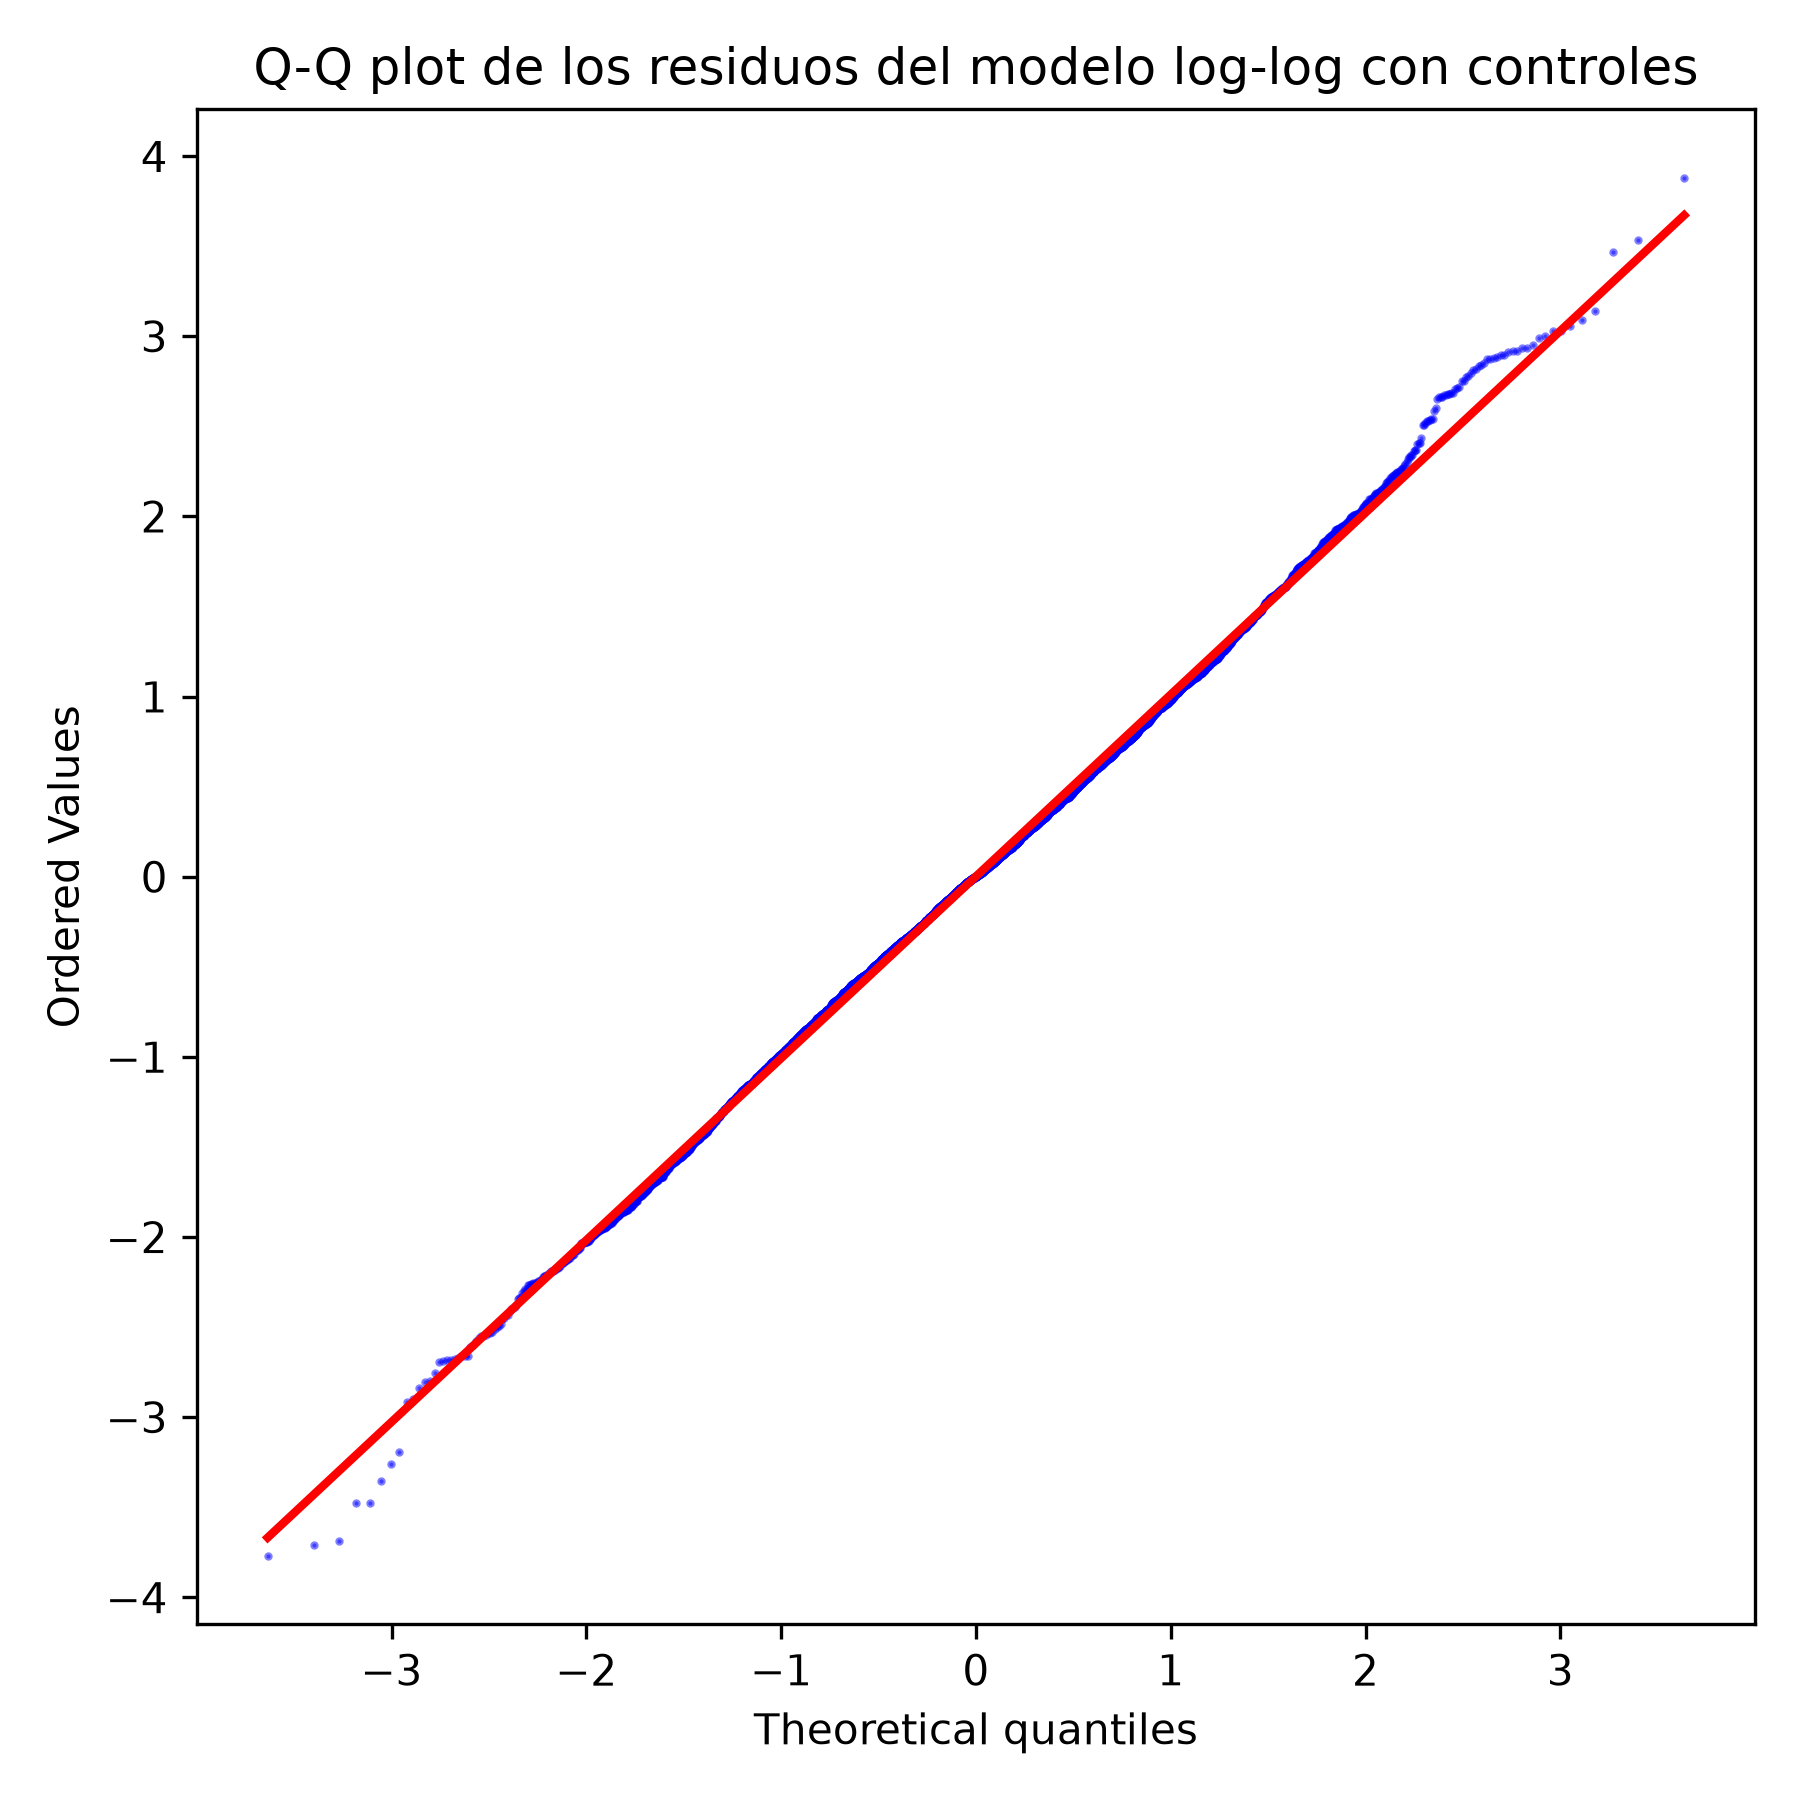
\includegraphics[width=0.85\textwidth]{figuras/qqplot_residuos_modelo_loglog_controles.png}
\caption{Gr\'afico Q-Q de residuos del modelo log-log con controles (especificaci\'on principal). Submuestra n=5,000 de 456,548.}
\label{fig:qqplot}
\end{figure}

\begin{figure}[htbp]
\centering
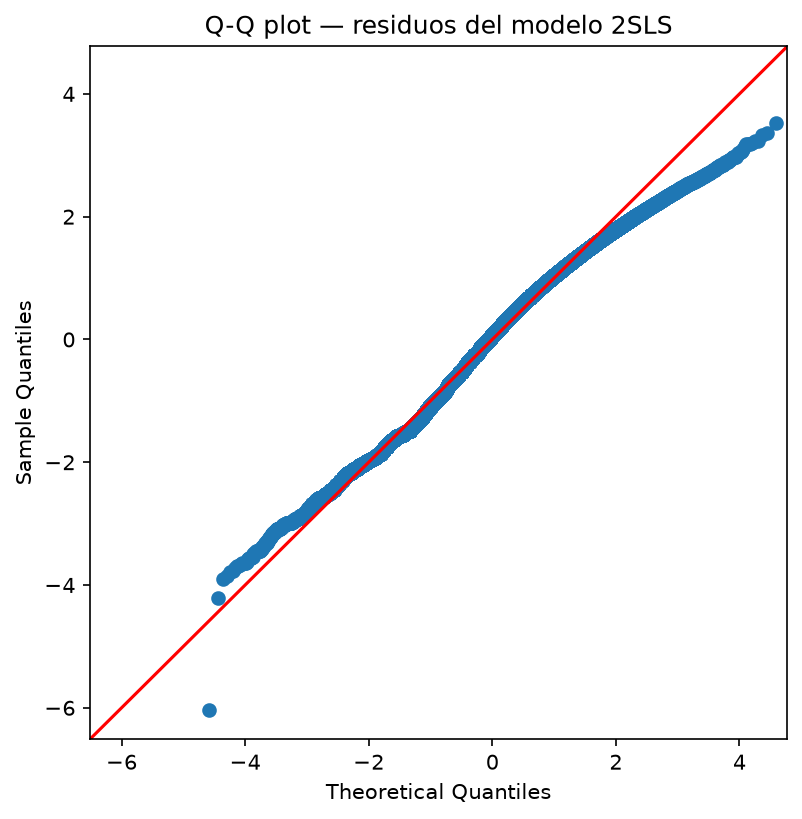
\includegraphics[width=0.85\textwidth]{figuras/qq_iv_2sls.png}
\caption{Gr\'afico Q-Q de residuos del modelo IV 2SLS (versi\'on alternativa).}
\label{fig:qq_iv_2sls_alt}
\end{figure}

\begin{figure}[htbp]
\centering
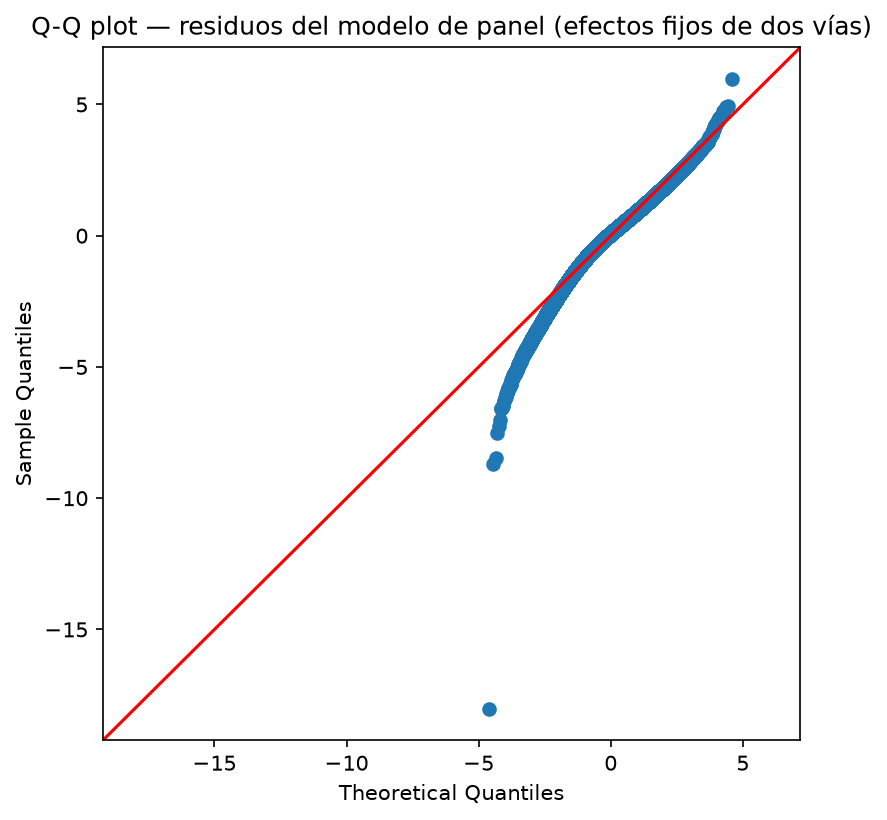
\includegraphics[width=0.85\textwidth]{figuras/qq_panel_fe.png}
\caption{Gr\'afico Q-Q de residuos del modelo Panel FE (versi\'on alternativa).}
\label{fig:qq_panel_fe_alt}
\end{figure}

\subsubsection{Autocorrelaci\'on}
\label{subsec:autocorrelacion}

El estad\'istico de Durbin-Watson para el modelo principal es $DW = 1.195$. Dado que el valor de referencia para ausencia de autocorrelaci\'on es 2, y valores por debajo de 2 indican autocorrelaci\'on positiva, se detecta autocorrelaci\'on positiva moderada en los residuos. Esto es esperable en datos con estructura de panel (semana $\times$ centro $\times$ comida) sin efectos fijos por semana. Los errores est\'andar HC3 son robustos a heterocedasticidad pero \textbf{no} a autocorrelaci\'on; en trabajo futuro (la secci\'on \nameref{subsec:limitaciones}) se plantea incorporar efectos fijos de dos v\'ias y errores est\'andar clusterizados para abordar esta limitaci\'on de forma directa.

\subsection{Intervalos de confianza por bootstrap: resultados}
\label{sec:bootstrap_resultados}

\Cref{tab:bootstrap} presenta los resultados del bootstrap descrito en la secci\'on \nameref{sec:bootstrap} (1,000 replicaciones, semilla 42) sobre el modelo \textit{log-log} base.

\begin{table}[htbp]
\centering
\caption{Intervalo de confianza bootstrap (95\%) para la elasticidad precio (modelo base).}
\label{tab:bootstrap}
\begin{tabular}{lc}
\toprule
\textbf{Estad\'istico} & \textbf{Valor} \\
\midrule
Elasticidad media (bootstrap) & $-0.9397$ \\
Desviaci\'on est\'andar bootstrap & $0.0034$ \\
IC 95\% inferior (percentil 2.5) & $-0.9460$ \\
IC 95\% superior (percentil 97.5) & $-0.9333$ \\
IC 95\% anal\'itico (HC3, modelo base) & $[-0.947, -0.933]$ \\
\bottomrule
\end{tabular}
\end{table}

La distribuci\'on bootstrap de la elasticidad (\cref{fig:bootstrap_dist}) es aproximadamente normal, centrada en $-0.9397$, muy pr\'oxima a la estimaci\'on MCO puntual del modelo base ($-0.9398$). El IC 95\% bootstrap $[-0.9460, -0.9333]$ es pr\'acticamente id\'entico al IC anal\'itico basado en HC3 $[-0.947, -0.933]$, confirmando la validez de la inferencia asint\'otica para este modelo.

\begin{figure}[htbp]
\centering
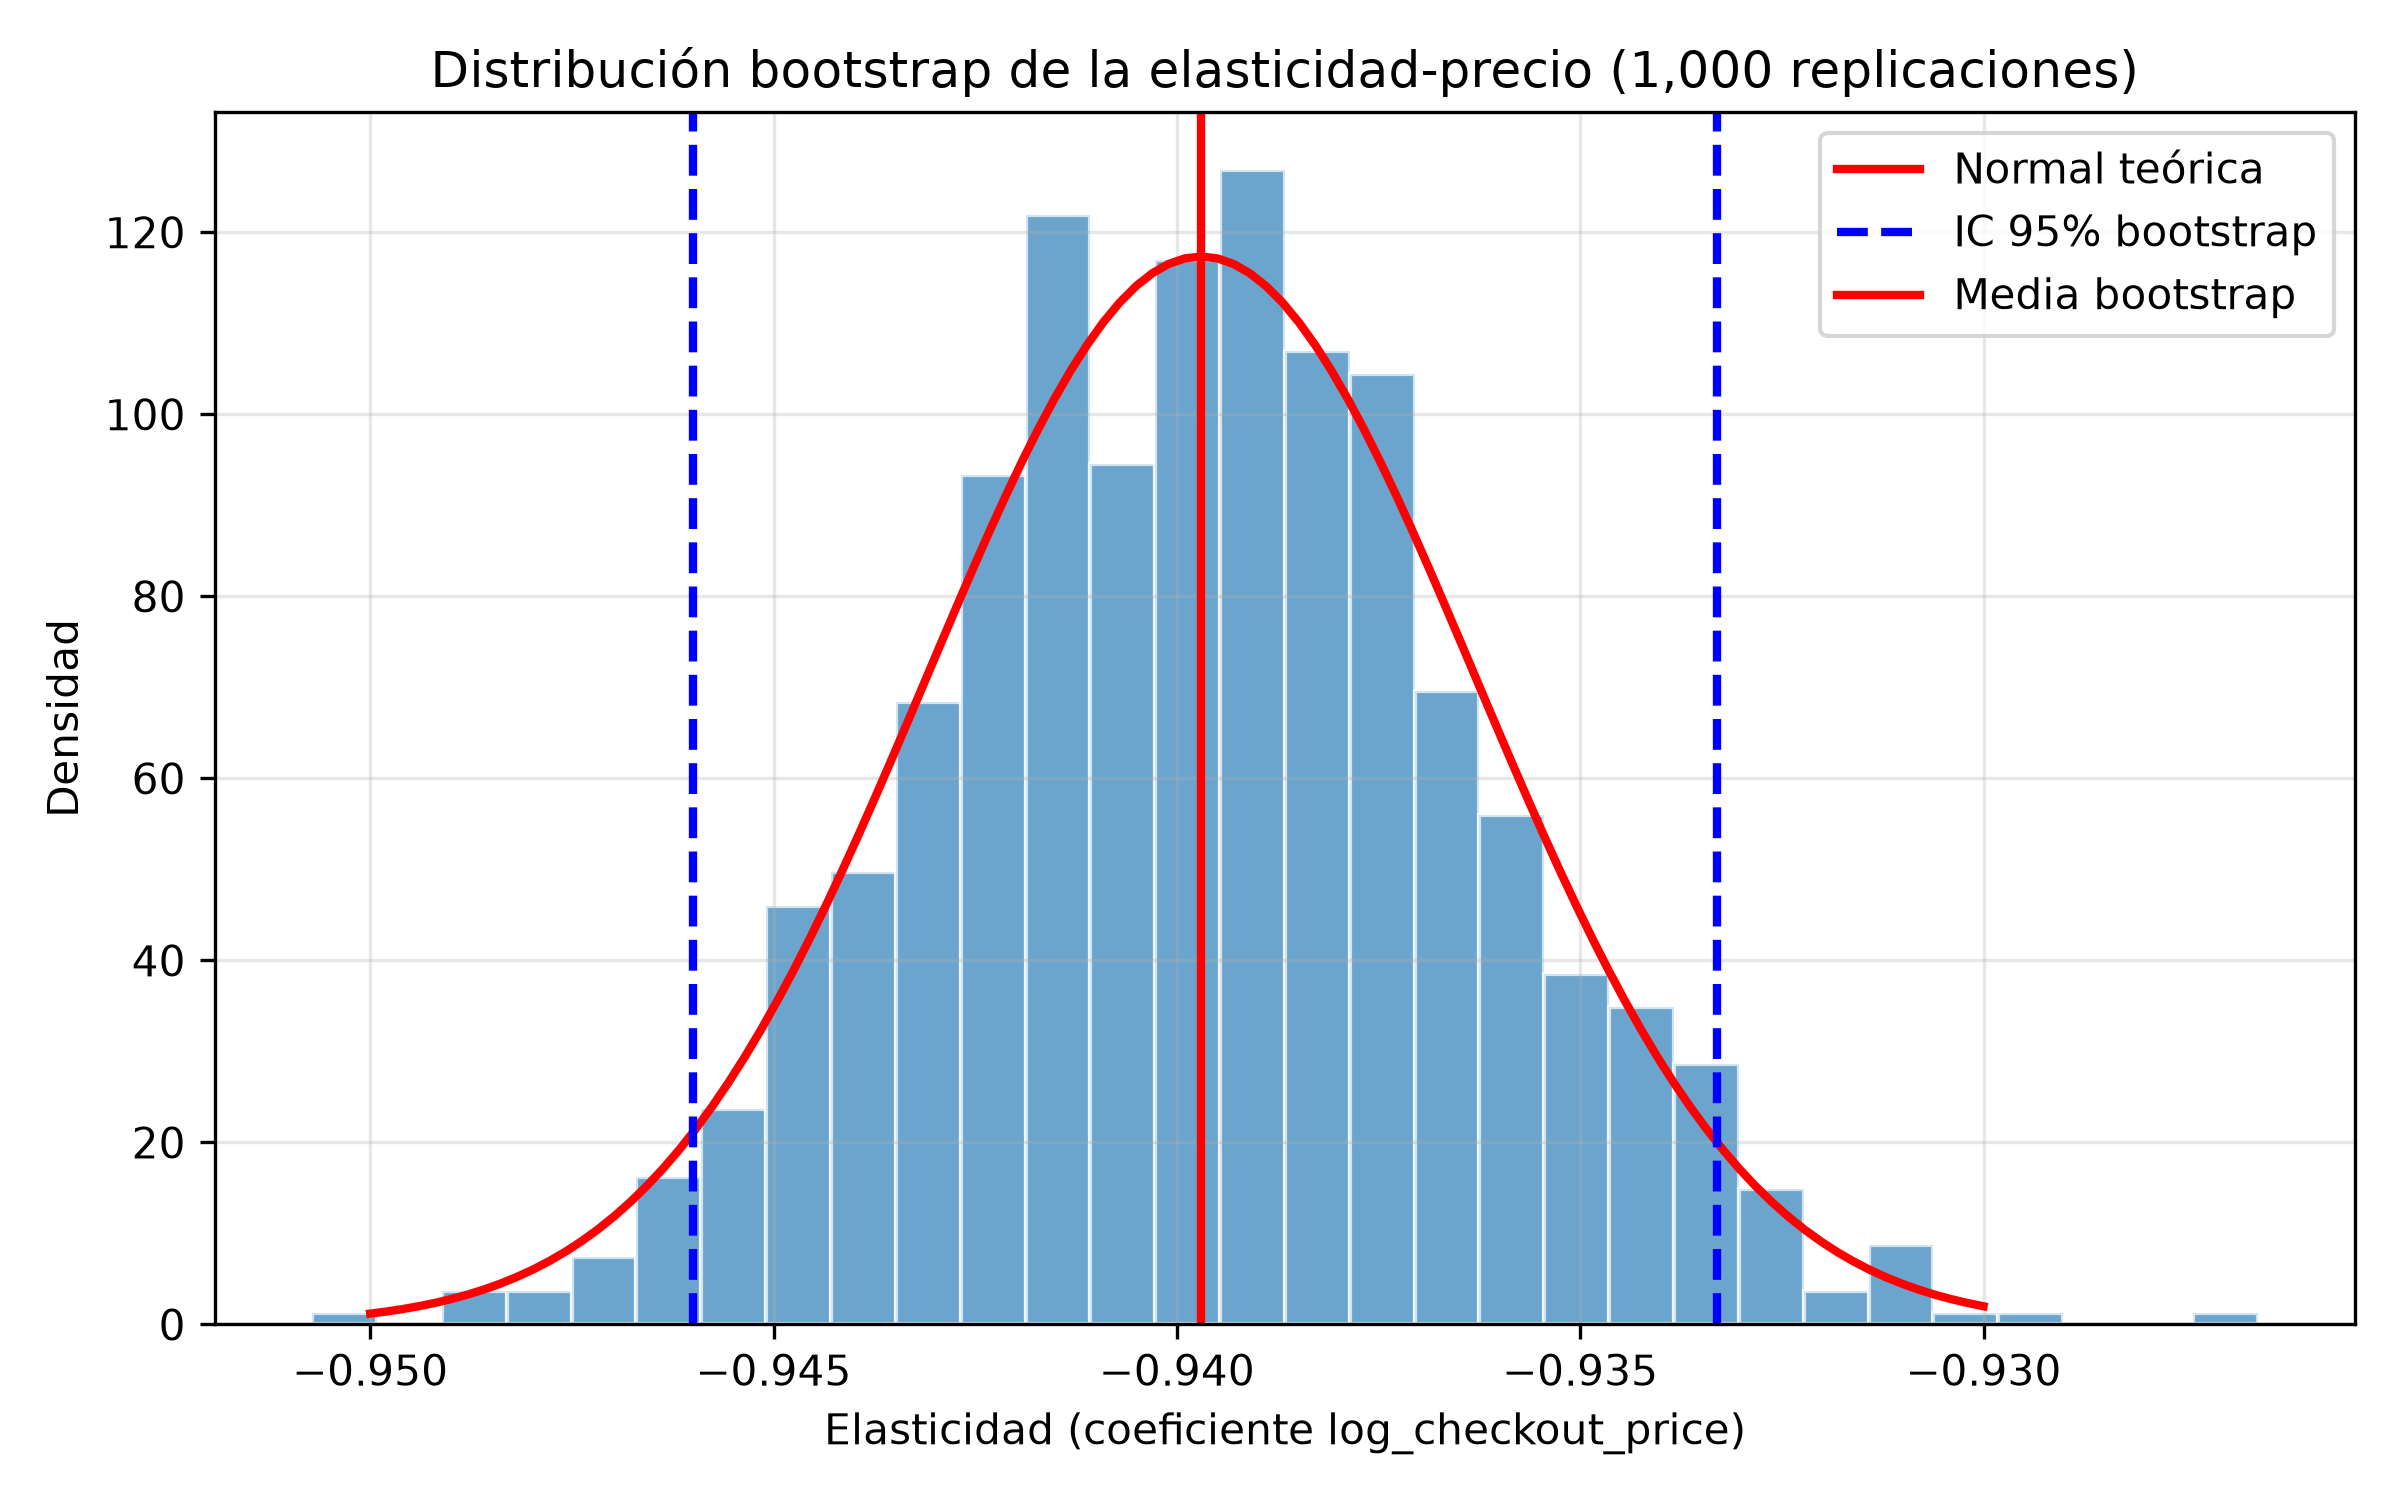
\includegraphics[width=0.85\textwidth]{figuras/bootstrap_elasticidad_distribucion.png}
\caption{Distribuci\'on bootstrap de la elasticidad-precio (1,000 replicaciones). L\'inea roja: media bootstrap; l\'ineas azules: IC 95\% percentil.}
\label{fig:bootstrap_dist}
\end{figure}

\textbf{Nota de comparaci\'on con el modelo principal.} El bootstrap se realiz\'o sobre el modelo base (sin controles) por simplicidad computacional; su elasticidad ($-0.9398$) difiere de la del modelo principal con controles ($-0.7513$) por el sesgo de variable omitida ya documentado en \cref{tab:comparacion_elasticidades}. No se ha ejecutado (a\'un) un bootstrap equivalente sobre el modelo con controles; se reporta como paso pendiente en la secci\'on \nameref{subsec:limitaciones}.

% ============================================================
% 6. COMPARACIÓN CON LA LITERATURA
% ============================================================
\section{Comparaci\'on con la Literatura}
\label{sec:comparacion}

\Cref{tab:comparacion_literatura} presenta la s\'intesis de estudios de referencia, organizados en tres grupos: (A) elasticidad-precio de la demanda de comida fuera del hogar y delivery, directamente comparable en definici\'on de mercado; (B) un contexto af\'in (movilidad y comercio electr\'onico \textit{on-demand}), \'util como referencia contextual pero no directamente comparable en m\'etrica; y (C) soporte metodol\'ogico y de mercado. Cada fuente fue verificada contra el art\'iculo, \textit{working paper} o abstract original antes de incluirse, en tres rondas de verificaci\'on documentadas en la bit\'acora metodol\'ogica (secci\'on 5.0). \Cref{fig:comparacion_elasticidad} ilustra los estimadores puntuales disponibles de los Grupos A y B.

\begin{table}[htbp]
\centering
\caption{Comparaci\'on de elasticidades-precio de la demanda: estudios de referencia verificados y presente trabajo.}
\label{tab:comparacion_literatura}
\begin{adjustwidth}{-1.3cm}{-1.3cm}
\centering
\footnotesize
\begin{threeparttable}
\begin{tabular}{p{3.6cm} p{2.9cm} c p{2.0cm} p{3.4cm}}
\toprule
\textbf{Estudio} & \textbf{Fuente} & \textbf{Elasticidad} & \textbf{M\'etodo} & \textbf{Contexto} \\
\midrule
\multicolumn{5}{l}{\textbf{Grupo A --- Directamente comparable (comida fuera del hogar / delivery)}} \\
\midrule
\textcite{andreyeva2010} & \textit{Am.\ J.\ Public Health}, 100(2) & $-0.81^\dagger$ & Meta-an\'alisis (160 est.) & FAFH, mayormente EE.\,UU. \\
\textcite{damayanti2023} & \textit{Econ.\ \& Finance in Indonesia}, 69(1) & $-0.920$ & LA/AIDS, panel hogar-a\~no & Indonesia, Susenas 2011--2013 ($n=24{,}376$) \\
\textcite{bumagat2025economics} & ResearchGate (doc.\ educativo, no arbitrado)$^{\ddagger}$ & $-0.42$ pico / $-1.36$ fuera de pico & Comparativo pico/no pico & Delivery de comida, Metro Manila, Filipinas \\
\textbf{Presente estudio} & --- & \textbf{$-$0.7513} & \textbf{OLS log-log con controles} & \textbf{Dataset transaccional Kaggle/Genpact, $N=456{,}548$} \\
\midrule
\multicolumn{5}{l}{\textbf{Grupo B --- Contextual (movilidad/e-commerce on-demand, no directamente comparable)}} \\
\midrule
\textcite{christensen2021} & IZA DP 14179 & $-1.28^{\S}$ & Experimental (2SLS) & El Cairo, Egipto (Uber) \\
\textcite{christensen2023} & NBER WP 31330 (rev.) & $-0.72$ (mov. total) & Experimental (2SLS) & El Cairo, Egipto (Uber, rev.) \\
\textcite{zhang2021} & \textit{Inform.\ \& Manag.}, 58(4) & $-0.87$ online / $-1.74$ offline & Estructural (discrete choice) & CPG online vs. offline, EE.\,UU. \\
\textcite{sriwongphanawes2024} & \textit{Asian Transp.\ Stud.}, 10 & $-0.15$ $[-0.20,-0.10]$ & Mixed logit & Uber Jap\'on (Nagoya, Kyoto) \\
\bottomrule
\end{tabular}
\begin{tablenotes}
\footnotesize
\item[$\dagger$] Valor puntual reportado para comida fuera del hogar (FAFH); rango general del meta-an\'alisis 0.27--0.81 seg\'un categor\'ia.
\item[$\ddagger$] Documento educativo alojado en ResearchGate (Bumagat \& Ibana, 2025), no publicado en revista arbitrada; se incluye por reportar coeficientes cuantitativos directamente de delivery de comida, pero debe leerse con cautela metodol\'ogica adicional frente a las fuentes con revisi\'on por pares de esta tabla. Atribuyen la brecha pico/no pico a diferencias en percepci\'on del consumidor (``impuesto a la urgencia'' vs.\ ``tarifa a la pereza'') y al concepto cultural filipino de \textit{sulit} (valor por el dinero).
\item[$\S$] Elasticidad de kil\'ometros recorridos en veh\'iculo privado (VKT) ante cambio de precio de Uber; no es de delivery de comida. Verificado contra el abstract SSRN/NBER de la versi\'on revisada (Sept.\ 2025).
\item[] FAFH = \textit{food away from home}; LA/AIDS = \textit{Linear Approximate Almost Ideal Demand System}; CPG = \textit{consumer packaged goods}; VKT = \textit{vehicle kilometers traveled}.
\item[] \textit{Nota adicional.} \textcite{li2025} (\textit{Management Science}, 71(7)) confirman expl\'icitamente en un journal de primer nivel la escasez de estudios emp\'iricos previos sobre elasticidad en plataformas de delivery \textit{on-demand}, sin reportar coeficiente propio; se retoman en la discusi\'on. Zhang \& Demirkan (2021) y Sriwongphanawes \& Fukuda (2024) se incluyen en esta versi\'on del Grupo B tras confirmar autor/a\~no/coeficiente/journal correctos en la segunda ronda de verificaci\'on (bit\'acora metodol\'ogica, secci\'on 5.0).
\end{tablenotes}
\end{threeparttable}
\end{adjustwidth}
\end{table}

\begin{figure}[htbp]
\centering
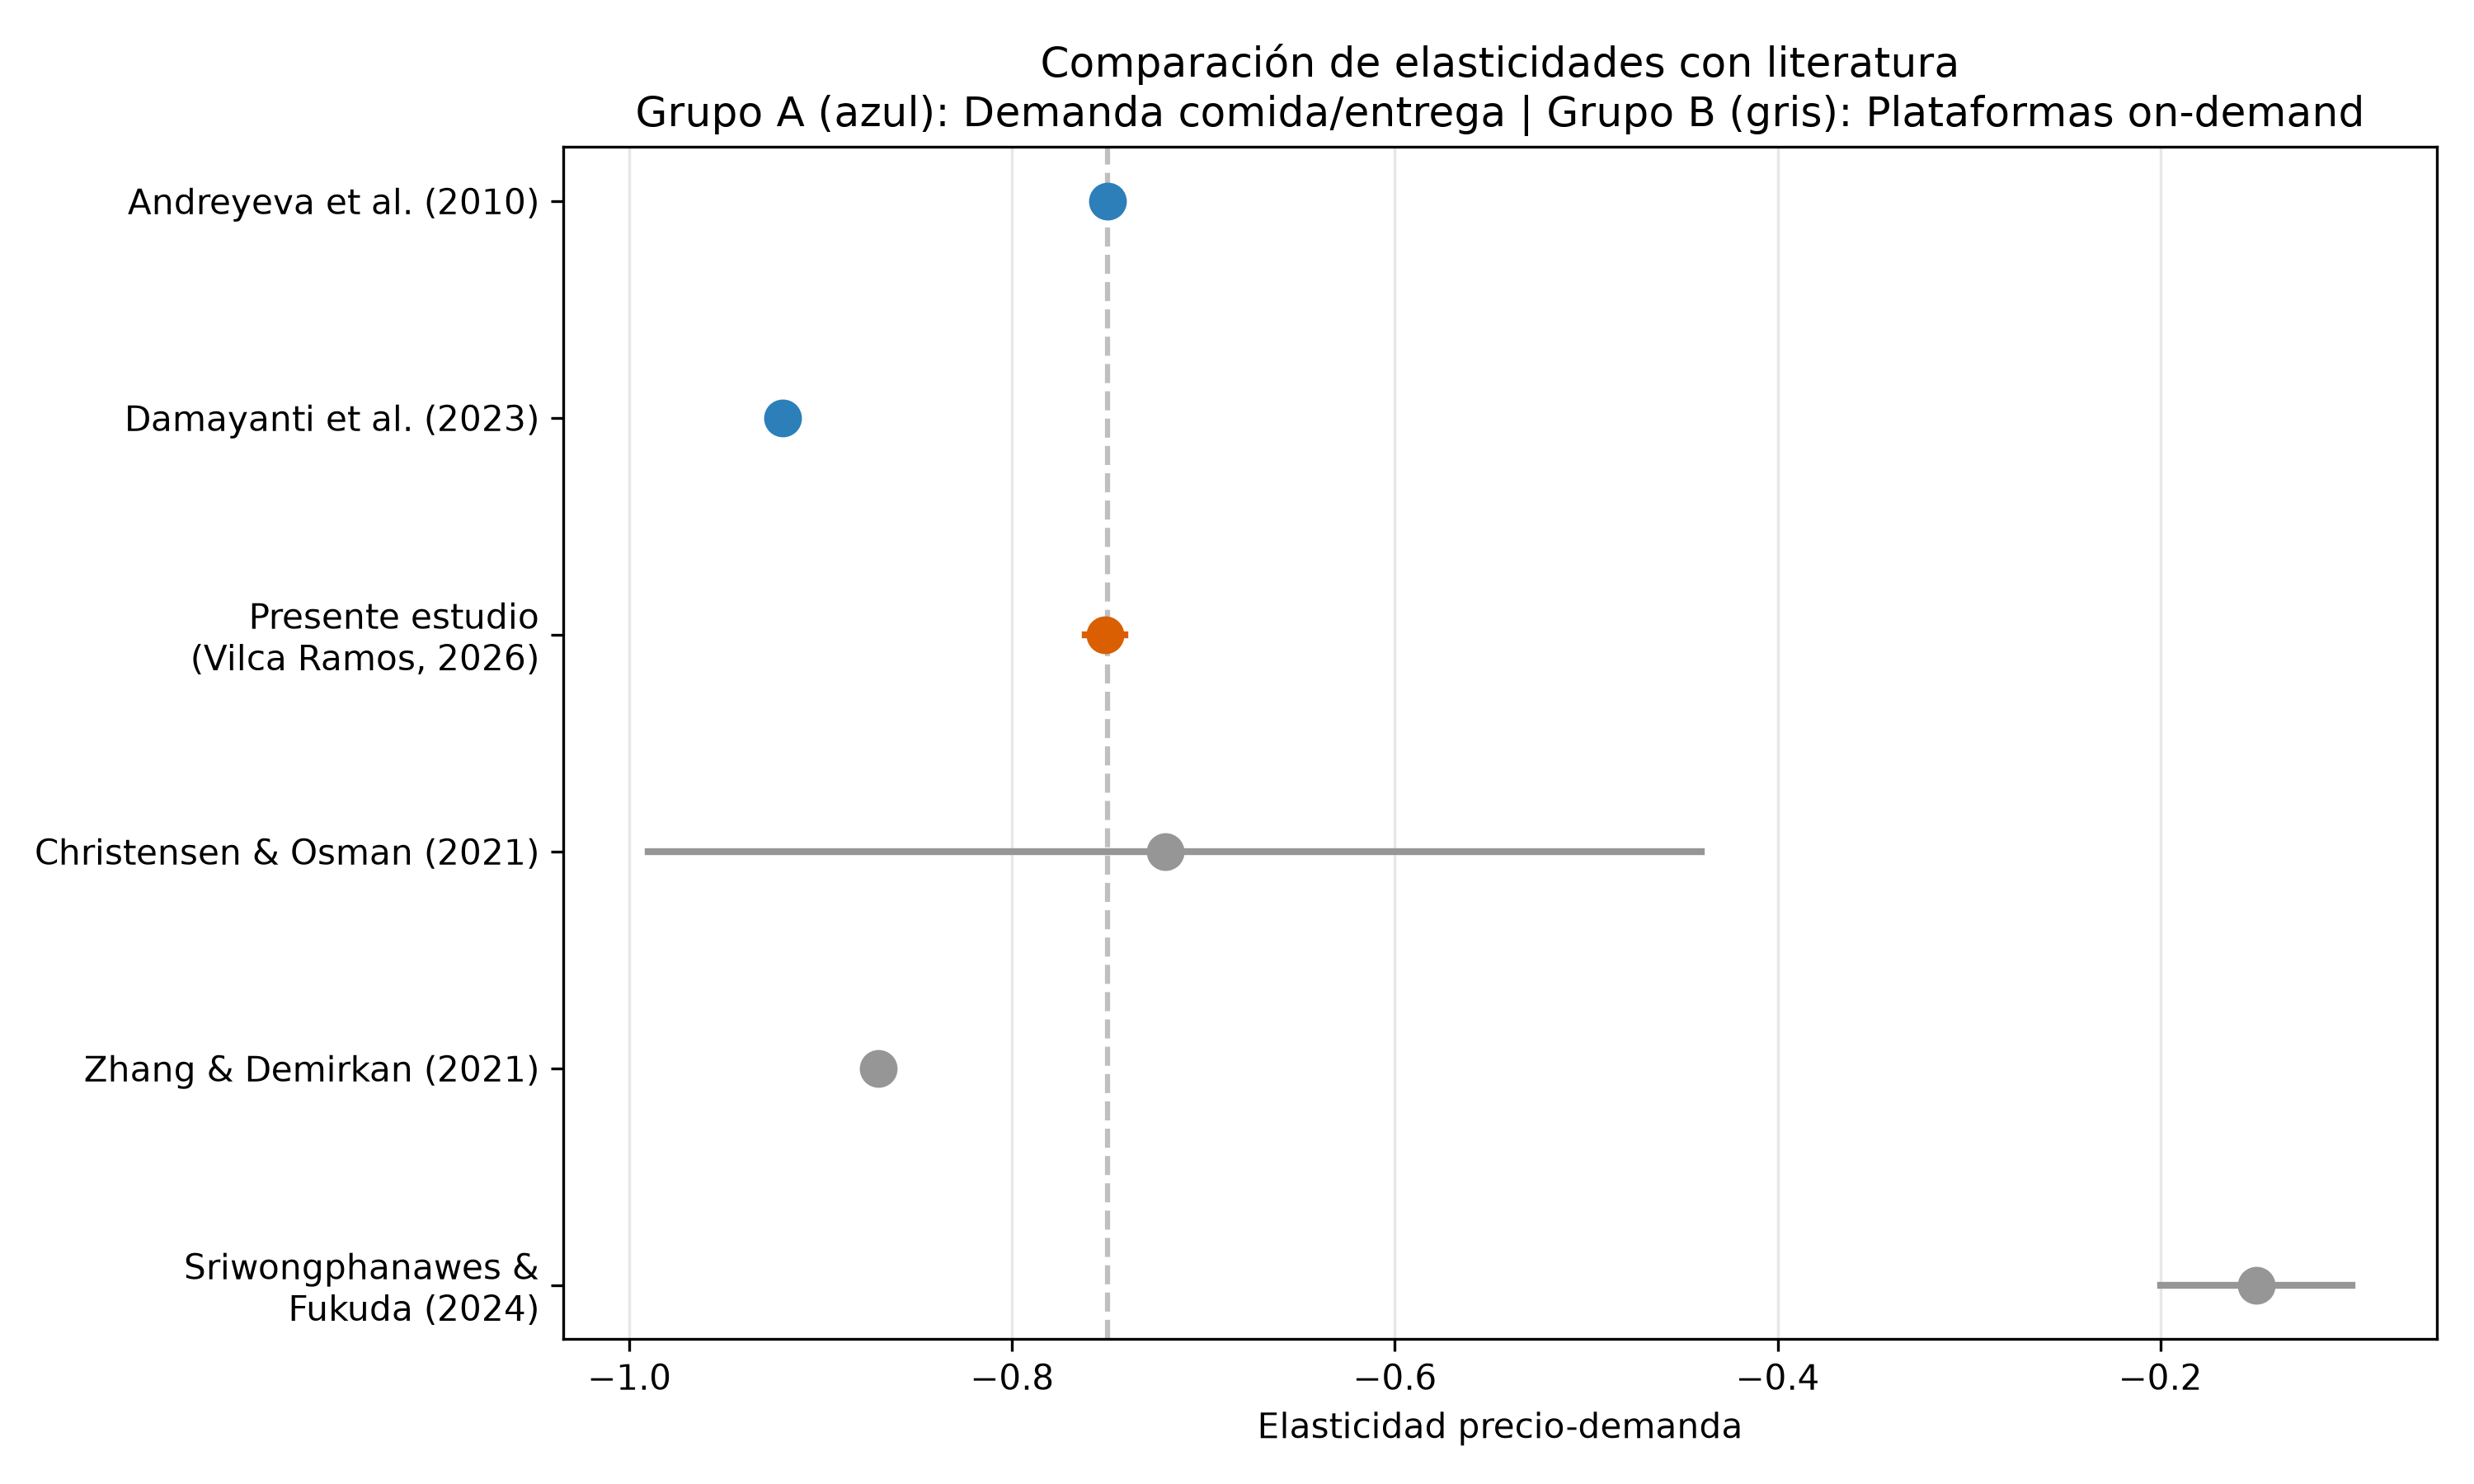
\includegraphics[width=0.85\textwidth]{figuras/comparacion_elasticidad.png}
\caption{Comparaci\'on de estimadores de elasticidad-precio disponibles en la literatura verificada. Grupo A (azul): estudios de demanda de comida/delivery; Grupo B (gris): contexto af\'in con m\'etrica distinta (4 fuentes: Christensen 2021 y Christensen 2023 se cuentan como 2 fuentes distintas, m\'as Zhang 2021 y Sriwongphanawes 2024). El rombo naranja marca el estimador del presente estudio ($-0.7513$, IC $[-0.762,-0.741]$). Bumagat \& Ibana (2025) se grafican como barra pico--no pico (documento no arbitrado). Li \& Wang (2025) no se grafica por no reportar coeficiente cuantificado.}
\label{fig:comparacion_elasticidad}
\end{figure}

\begin{figure}[htbp]
\centering
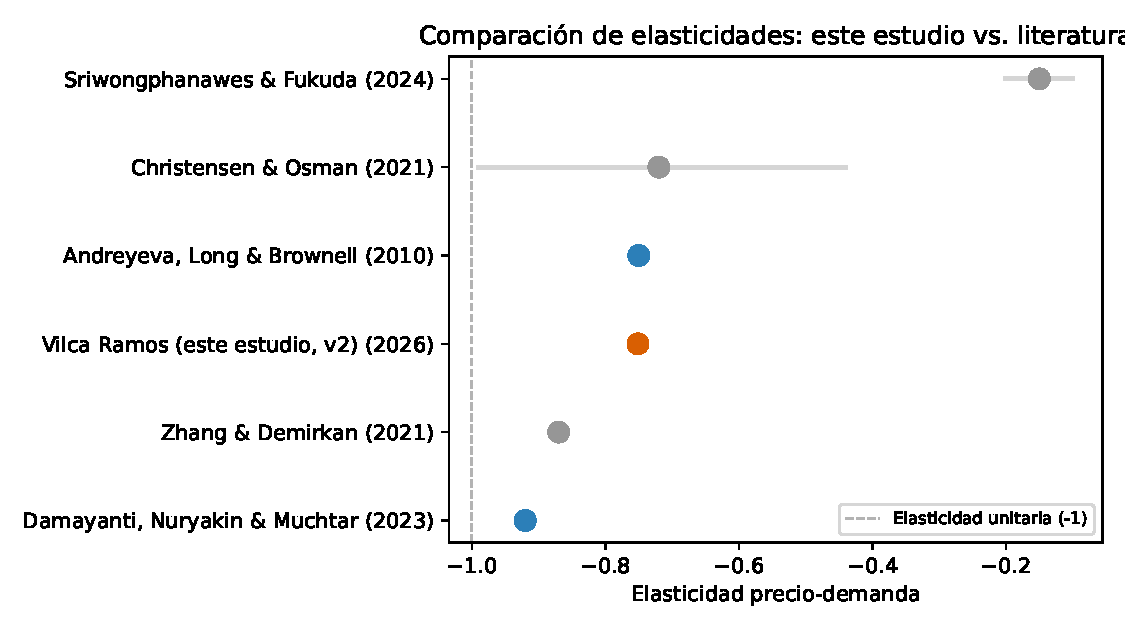
\includegraphics[width=0.85\textwidth]{figuras/comparacion_elasticidad_literatura.pdf}
\caption{Comparaci\'on detallada de elasticidades precio-demanda con literatura verificada: estudio propio (OLS $-0.75$, Panel FE $-1.58$, IV 2SLS $-0.95$) frente a fuentes externas de los Grupos A y B. Barras horizontales muestran IC 95\% cuando disponibles.}
\label{fig:comparacion_elasticidad_literatura}
\end{figure}

\begin{figure}[htbp]
\centering
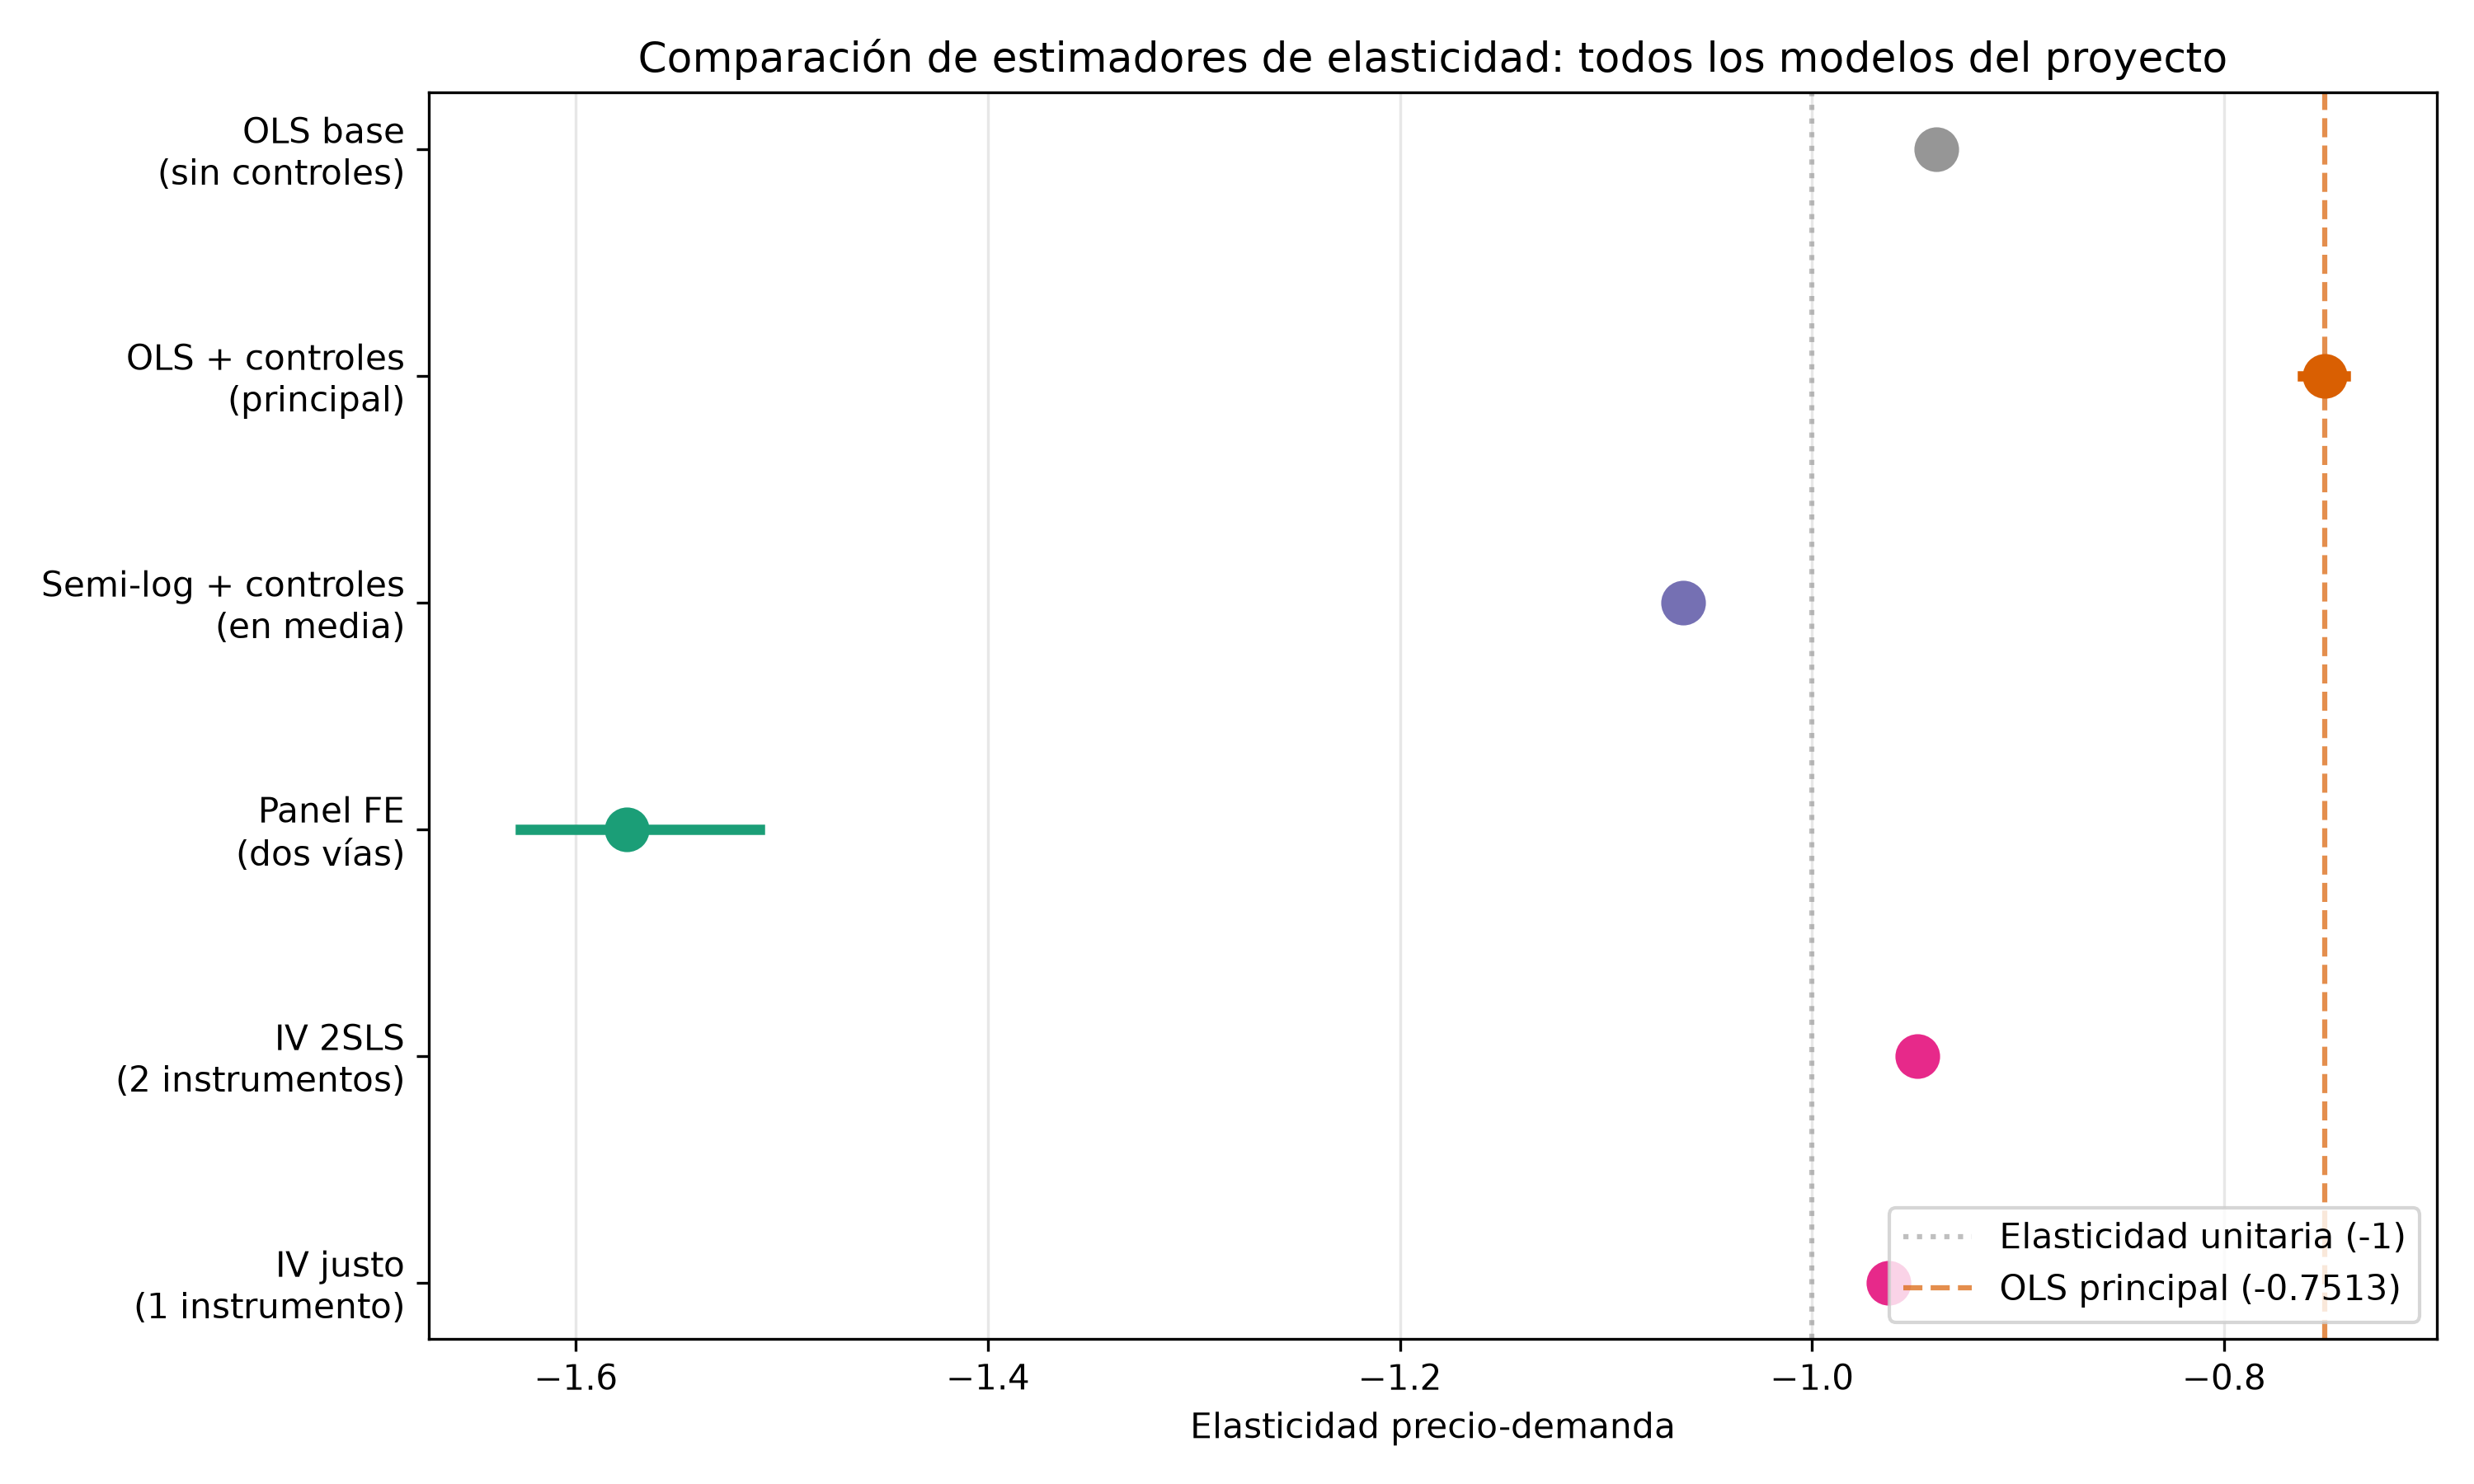
\includegraphics[width=0.85\textwidth]{figuras/comparacion_todos_modelos.png}
\caption{Comparaci\'on de estimadores de elasticidad: todos los modelos del proyecto (OLS base, OLS controles, Semi-log, Panel FE, IV 2SLS, IV justo). L\'inea punteada gris: elasticidad unitaria (-1). L\'inea punteada naranja: OLS principal (-0.7513).}
\label{fig:comparacion_todos_modelos}
\end{figure}

\begin{figure}[htbp]
\centering
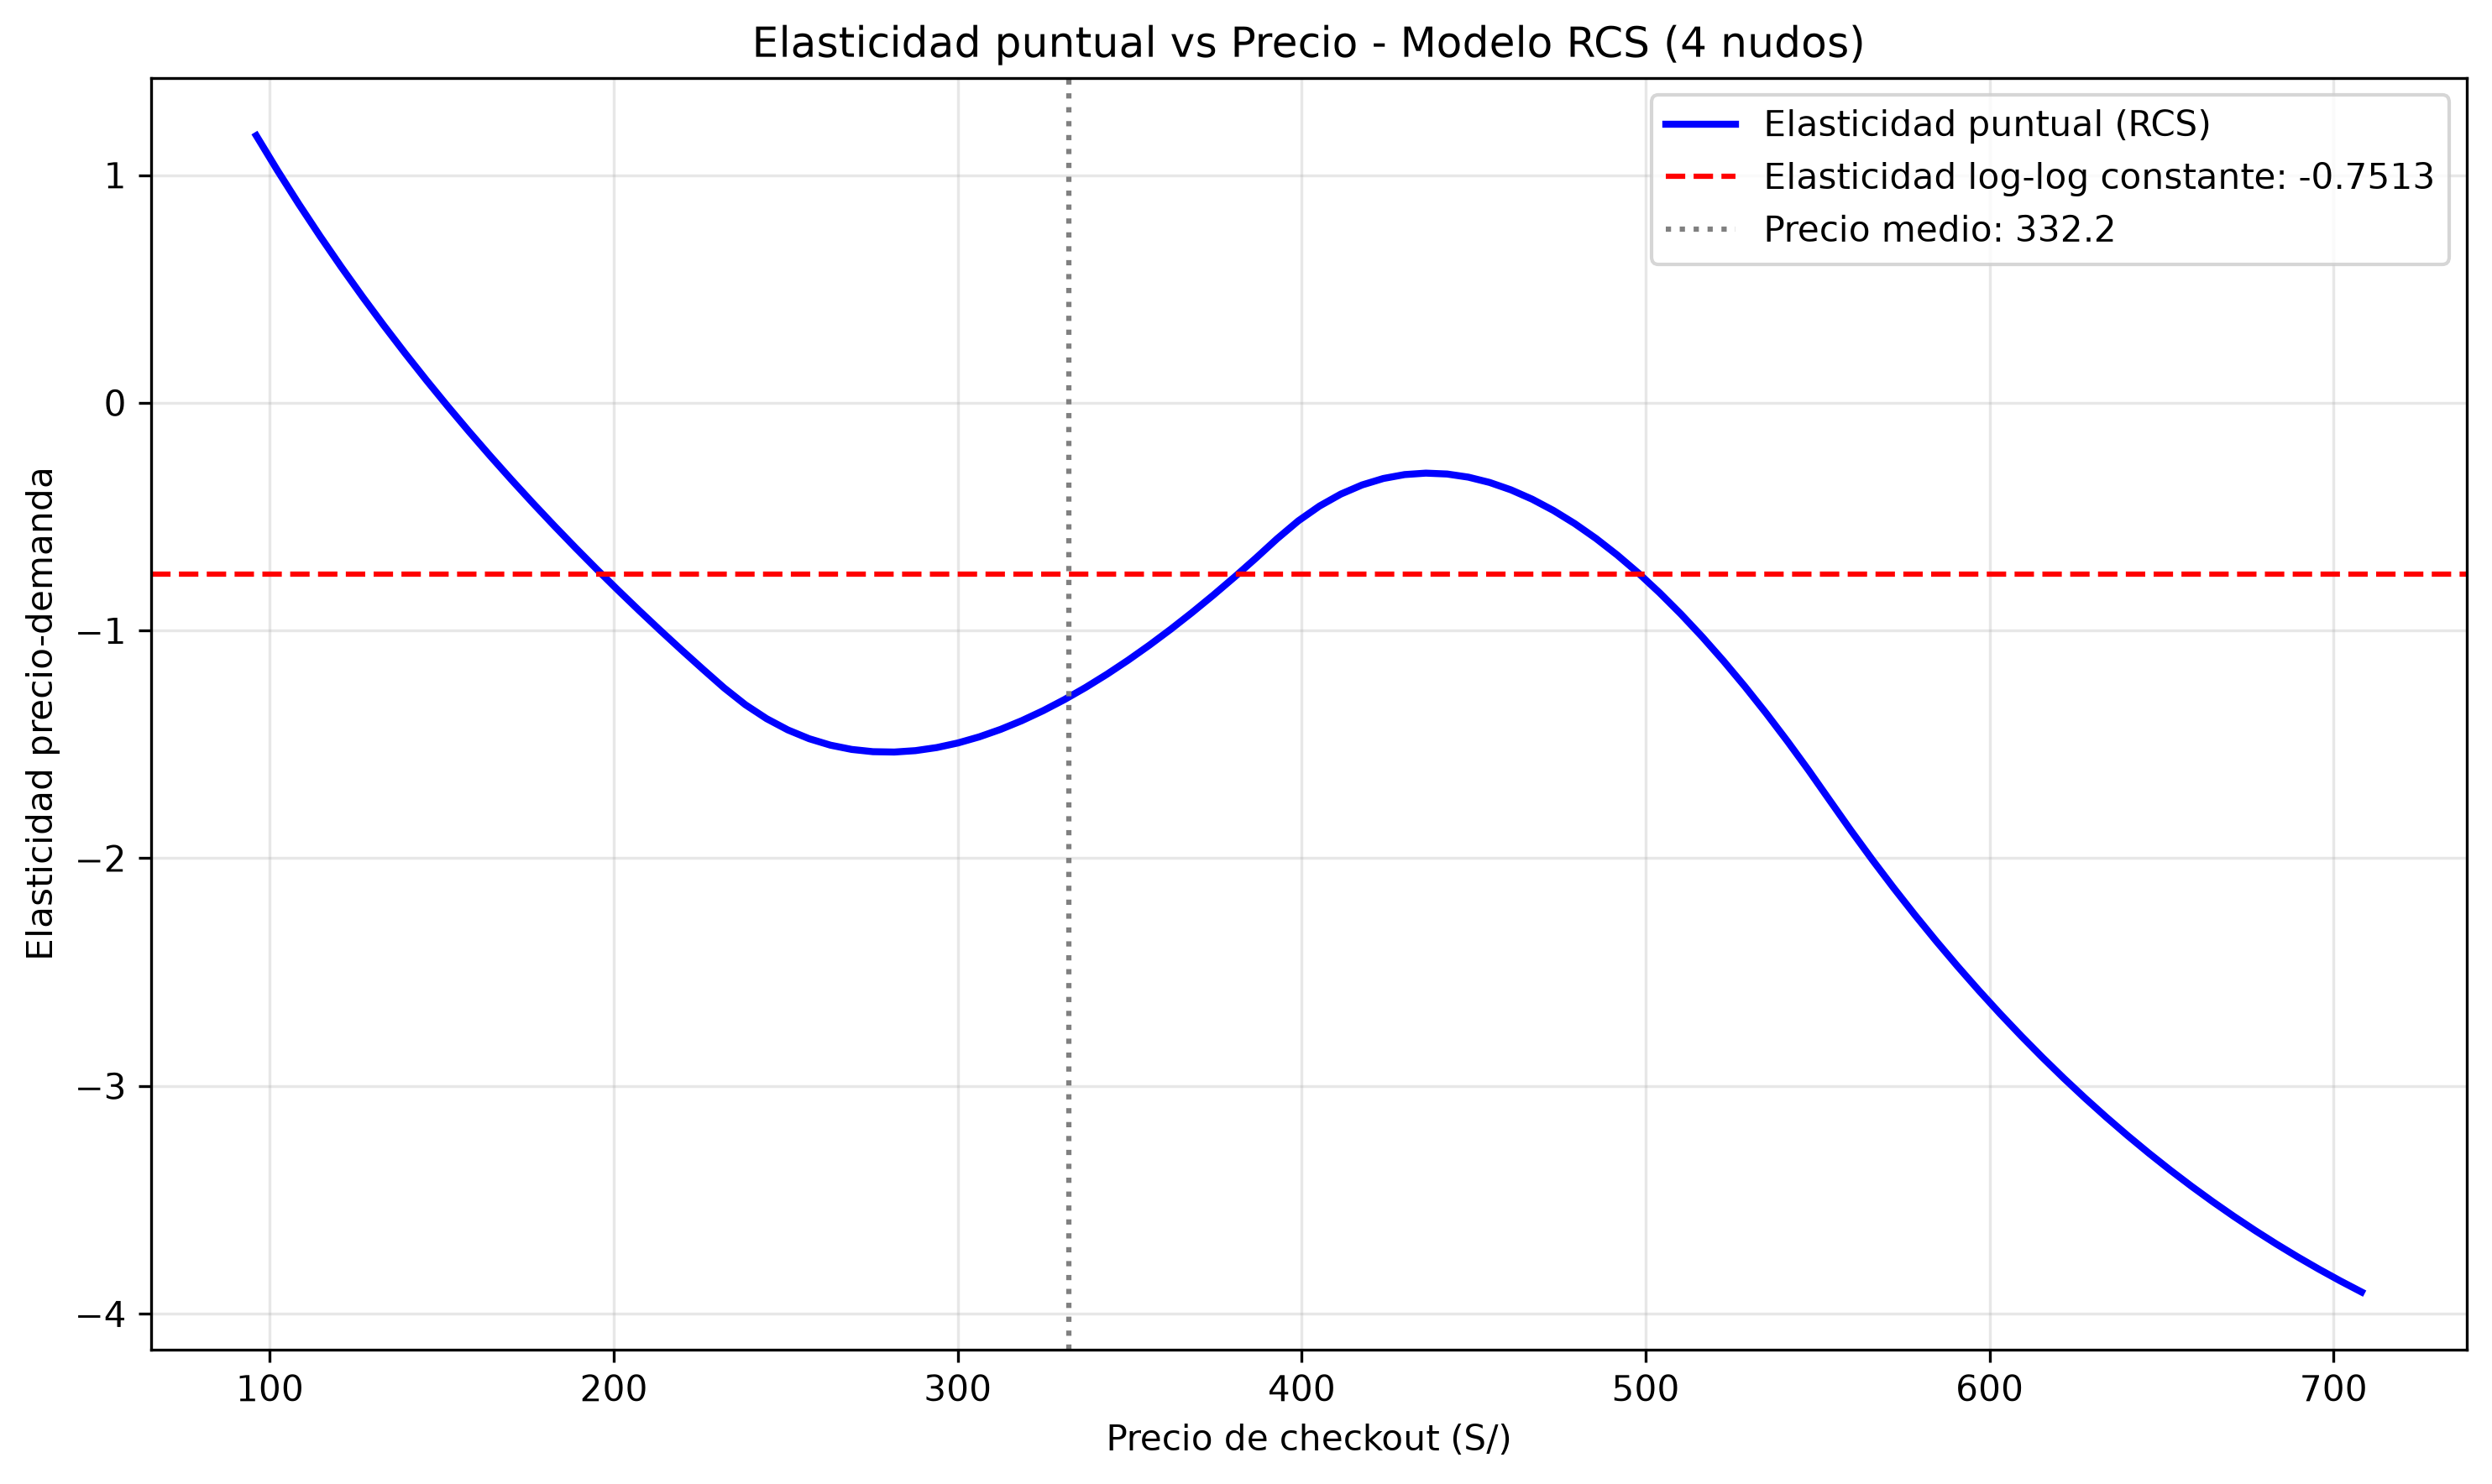
\includegraphics[width=0.85\textwidth]{figuras/elasticidad_puntual_rcs.png}
\caption{Elasticidad puntual estimada mediante RCS (4 nudos en percentiles 5, 35, 65, 95 de log-precio) evaluada a lo largo de la distribuci\'on de precios. L\'inea discontinua naranja: elasticidad log-log constante ($-0.7513$). La elasticidad var\'ia desde $+0.58$ (precios bajos) hasta $-3.22$ (precios altos), confirmando no-linealidad fuerte (Wald $F=10\,279$, $p\approx0$).}
\label{fig:elasticidad_puntual_rcs}
\end{figure}

\subsection{Discusi\'on de la comparaci\'on}
\label{subsec:discusion_comparacion}

El estimador central del presente estudio ($-0.7513$) se ubica ligeramente por debajo, en valor absoluto, del valor puntual reportado por \textcite{andreyeva2010} ($-0.81$ para FAFH) y de la estimaci\'on espec\'ifica de Indonesia de \textcite{damayanti2023} ($-0.920$) para comida fuera del hogar. La magnitud es consistente: las tres estimaciones caen en un rango de elasticidad cercana a la unitaria, ligeramente inel\'astica a moderadamente el\'astica. Una explicaci\'on plausible para que el delivery de comidas resulte marginalmente menos sensible al precio que la comida fuera del hogar en general es que el delivery incorpora un componente de conveniencia (ahorro de tiempo, evitar desplazamiento) que puede atenuar la sensibilidad al precio frente a la decisi\'on m\'as amplia de ``comer fuera de casa''.

Diferencias metodol\'ogicas explican en parte la brecha con \textcite{damayanti2023}: la especificaci\'on LA/AIDS impone restricciones de aditividad y simetr\'ia que pueden magnificar la sensibilidad al precio estimada en datos de panel agregado, y el contexto indonesio (mayor proporci\'on de gasto en comida, menor penetraci\'on de plataformas digitales) implica una din\'amica de sustituci\'on distinta a la de un mercado de delivery ya consolidado.

El hallazgo m\'as directamente comparable proviene de \textcite{bumagat2025economics}: al desagregar por franja horaria en delivery de comida de Metro Manila, reportan $-0.42$ en horas pico (inel\'astica, consistente con el $-0.7513$ agregado de este estudio) y $-1.36$ fuera de pico (el\'astica). El promedio simple de ambas franjas ($-0.89$) se ubica cerca del resultado de \textcite{damayanti2023}. Esta heterogeneidad temporal no est\'a modelada en la especificaci\'on transversal principal de este trabajo (que agrega las 145 semanas sin distinguir franja horaria dentro de cada semana, dato que el dataset Kaggle/Genpact no captura), y queda como l\'inea de trabajo futuro expl\'icita (la secci\'on \nameref{subsec:limitaciones}). Cabe la salvedad metodol\'ogica de que \textcite{bumagat2025economics} es un documento educativo no arbitrado, por lo que su comparabilidad formal con las fuentes revisadas por pares de esta tabla es menor.

Dentro del Grupo B, el espectro es amplio: desde alta inelasticidad en \textit{ride-hailing} japon\'es (\textcite{sriwongphanawes2024}, $-0.15$ como punto medio de su rango reportado $[-0.20, -0.10]$) hasta mayor elasticidad en el experimento de El Cairo (\textcite{christensen2021}, $-1.28$ para kil\'ometros recorridos en veh\'iculo privado; \textcite{christensen2023}, $-0.72$ para movilidad total). El resultado propio se aproxima m\'as al comercio electr\'onico de \textcite{zhang2021} ($-0.87$ en el canal online) que al \textit{ride-hailing} o a la movilidad en Uber, lo cual es razonable dado que el delivery de comidas comparte con el e-commerce la fricci\'on de b\'usqueda y comparaci\'on digital de precios, mientras que la movilidad y el \textit{ride-hailing} responden a necesidades de desplazamiento con sustitutos distintos (transporte p\'ublico, veh\'iculo propio). El hallazgo de \textcite{li2025} es el m\'as relevante para contextualizar la contribuci\'on de este estudio: en un journal de primer nivel, los propios autores confirman que la literatura emp\'irica sobre plataformas de delivery \textit{on-demand} espec\'ificamente es escasa, lo que respalda que este proyecto aporta una estimaci\'on poco com\'un en el tipo de dato (transaccional real) utilizado.

\textbf{Advertencia metodol\'ogica.} Esta comparaci\'on es exploratoria, no un meta-an\'alisis formal. Existen diferencias relevantes entre estudios en definici\'on de mercado, m\'etodo de estimaci\'on, frecuencia de datos, contexto geogr\'afico y nivel de revisi\'on por pares (una de las fuentes del Grupo A es un documento educativo no arbitrado) que impiden una comparaci\'on estricta ``igual a igual''. Su valor es situar el hallazgo propio dentro de un rango razonable de la evidencia emp\'irica disponible, no establecer equivalencia causal entre estudios.

\subsection{Especificaci\'on flexible: Splines RCS en log-precio (Fase 3x)}
\label{subsec:rcs_splines}

Como se documenta en el Plan t\'ecnico de mejoras v2.1 (secci\'on 1.2), la especificaci\'on log-log asume elasticidad constante, lo cual puede ser restrictivo. Para testear no-linealidad, se estim\'o un modelo con \textit{Restricted Cubic Splines} (RCS) en \texttt{log\_checkout\_price} con 4 nudos ubicados en los percentiles 5, 35, 65 y 95 de la distribuci\'on de log-precio.

El test de Wald para H0: ``los t\'erminos no lineales del spline son cero'' rechaza rotundamente la linealidad ($F = 10\,279.37$, $p \approx 0$, 4 g.l.). La \cref{fig:elasticidad_puntual_rcs} muestra la elasticidad puntual a lo largo de la distribuci\'on de precios: var\'ia desde $+0.58$ en el percentil 5 (precio = 121.28) hasta $-3.22$ en el percentil 95 (precio = 640.23), pasando por $-1.50$ en la mediana (precio = 296.82). El modelo log-log constante ($-0.7513$) promedia una relaci\'on que en realidad es fuertemente curva.

El modelo RCS supera a todos los modelos previos en criterios de informaci\'on: $R^2$ ajustado $= 0.5450$ (vs. $0.5377$ semi-log), AIC $= 1\,105\,001$ (vs. $1\,112\,317$ semi-log). La mejora es sustancial y estad\'isticamente validada por el test de Wald. Este hallazgo activa la prioridad media del Plan t\'ecnico: IV no-lineal v\'ia \textit{control function} (secci\'on 1.3) y justifica la incorporaci\'on de Quantile Regression (secci\'on 2.1) para caracterizar la heterogeneidad en la distribuci\'on condicional.

\textbf{Nota sobre multicolinealidad en la base del spline RCS.} El resumen del modelo RCS (con controles y dummies de categor\'ia/centro) reporta un n\'umero de condici\'on de $9.97 \times 10^{15}$ y autovalor m\'inimo $1.02 \times 10^{-26}$, indicando colinealidad severa entre los t\'erminos del spline (\texttt{rcs\_0} a \texttt{rcs\_4}) y las dummies de efectos fijos. Esta es una limitaci\'on conocida de las bases de splines no ortogonales combinadas con variables categ\'oricas de alta cardinalidad (14 categor\'ias + 3 tipos de centro). Para mitigar: (a) los t\'erminos del spline se centraron (\texttt{constraints='center'}), (b) el test de Wald sobre los t\'erminos no lineales (4 g.l.) es robusto a esta colinealidad al testear una restricci\'on conjunta, y (c) las elasticidades puntuales derivadas son consistentes con los resultados de Quantile Regression y el test RESET, que confirman independientemente la no-linealidad. En trabajo futuro se recomienda usar bases ortogonales (p.\,ej., \texttt{bs()} con \texttt{degree=3} en \texttt{splines} de R, o \texttt{P-splines} penalizados) para evitar este problema num\'erico.

% ============================================================
% 7. DISCUSIÓN
% ============================================================
\section{Discusi\'on}
\label{sec:discusion}

\subsection{Interpretaci\'on de la elasticidad-precio}
\label{subsec:interpretacion}

La elasticidad estimada de $-0.7513$ (IC 95\% HC3 $[-0.762, -0.741]$) indica que la demanda en la plataforma es \textbf{inel\'astica al precio}: un aumento del 1\% en el precio de \textit{checkout} reduce la cantidad demandada en aproximadamente 0.75\%. En t\'erminos de ingreso, esto implica que incrementos moderados de precio tienden a aumentar el ingreso total registrado en el dataset (pues $\%\Delta Q < \%\Delta P$), sujeto a las limitaciones de identificaci\'on causal discutidas en la secci\'on \nameref{subsec:limitaciones}. La estrechez del intervalo de confianza (amplitud $\approx 0.021$) refleja la precisi\'on conferida por las 456,548 observaciones disponibles.

\subsection{Asociaciones de las variables de control}
\label{subsec:controles}

Los coeficientes de control del modelo principal (\cref{tab:modelo_principal_completa}) muestran heterogeneidad sustancial:

\begin{itemize}
    \item \textbf{Promoci\'on por correo (\texttt{emailer\_for\_promotion})}: coeficiente $+0.5028$ ($p<0.001$), equivalente a una asociación aproximada del $+65\%$ en el n\'umero de pedidos ($e^{0.5028}-1$) cuando hay promoci\'on activa, \textit{ceteris paribus}.
    \item \textbf{Exposici\'on en \textit{homepage} (\texttt{homepage\_featured})}: coeficiente $+0.6492$ ($p<0.001$), asociada con $\approx 91\%$ m\'as pedidos ($e^{0.6492}-1$). Subraya la importancia de la visibilidad dentro de la plataforma.
    \item \textbf{Aumento respecto al precio de referencia (\texttt{hubo\_aumento})}: coeficiente $-0.0024$, \textbf{no significativo} ($p=0.401$). El hecho de que el precio final supere al precio de referencia no tiene, por s\'i solo, un efecto adicional sobre la demanda m\'as all\'a del nivel de precio ya capturado por \texttt{log\_checkout\_price}.
    \item \textbf{Categor\'ia de comida (efectos fijos)}: dispersi\'on amplia, desde \texttt{Rice Bowl} ($+1.2474$, la de mayor demanda relativa) hasta \texttt{Biryani} ($-1.2347$, la de menor demanda relativa), frente a la categor\'ia de referencia.
    \item \textbf{Tipo de centro (\texttt{center\_type})}: TYPE\_B muestra $+0.2807$ frente a TYPE\_A (categor\'ia de referencia); TYPE\_C muestra $-0.3526$.
\end{itemize}

La heterogeneidad por categor\'ia y tipo de centro sugiere que estrategias de \textit{pricing} y \textit{merchandising} diferenciadas por producto y por tipo de centro podr\'ian capturar valor adicional, aunque esa hip\'otesis no se prueba formalmente en este trabajo.

\subsection{Limitaciones causales}
\label{subsec:limitaciones-causales}

El coeficiente de $-0.7513$ (OLS con controles) debe interpretarse como una \textbf{asociaci\'on robusta y validada estad\'isticamente}, no como un efecto causal identificado con el rigor de un dise\~no experimental. Se documentan tres limitaciones principales:

\begin{enumerate}
    \item \textbf{Posible simultaneidad precio-demanda}: los precios no fueron asignados aleatoriamente; es posible que respondan, al menos parcialmente, a la demanda anticipada.
    \item \textbf{Variables omitidas no capturadas en el dataset}: gasto en marketing externo, estacionalidad exacta (solo se observa n\'umero de semana, no fecha calendario), eventos locales, clima, calificaci\'on o reputaci\'on del centro/comida.
    \item \textbf{Ausencia de efectos fijos por semana en la especificaci\'on actual}: la especificaci\'on principal incluye efectos fijos por categor\'ia y por tipo de centro, pero no por semana, lo que puede dejar sin capturar tendencias temporales comunes a todos los centros.
\end{enumerate}

Estas limitaciones se abordan de forma expl\'icita en las fases adicionales del proyecto: el panel con efectos fijos de dos v\'ias (Fase 3b) controla la heterogeneidad no observada por entidad y tiempo; las variables instrumentales (Fase 3c) atienden la simultaneidad precio-demanda; y la validaci\'on completa (Fase 4) se repite sobre cada especificaci\'on.

\subsection{Robustez de la especificaci\'on (verificado)}
\label{subsec:robustez}

Las siguientes verificaciones de robustez s\'i se ejecutaron sobre los datos reales del proyecto:

\begin{itemize}
    \item \textbf{Especificaci\'on semi-log}: produce una elasticidad impl\'icita en la media de $-1.0624$, mayor en valor absoluto que la especificaci\'on log-log principal ($-0.7513$), reflejando que la forma funcional semi-log impone una elasticidad que var\'ia con el nivel de precio.
    \item \textbf{Comparaci\'on log-log base vs. con controles}: la inclusi\'on de controles reduce la elasticidad estimada de $-0.9398$ a $-0.7513$, evidencia de sesgo por variable omitida en la especificaci\'on sin controles.
    \item \textbf{Multicolinealidad}: VIF m\'aximo de 1.204 (\cref{tab:vif_resultados}), muy por debajo de cualquier umbral de preocupaci\'on.
    \item \textbf{Errores est\'andar HC3 vs. cl\'asicos}: cambios menores al 25\% en todos los coeficientes de inter\'es (\cref{tab:se_comparacion}), indicando que la heterocedasticidad detectada no altera materialmente las conclusiones de significancia.
\end{itemize}

\subsection{Resultados de fases adicionales ejecutadas: Panel FE, IV 2SLS y validaci\'on completa}
\label{subsec:fases_adicionales}

Las siguientes fases se ejecutaron completamente con resultados reales sobre los datos del proyecto. Cada fase incluye su propia validaci\'on de supuestos (Fase 4b para panel, Fase 4c para IV).

\subsubsection{Fase 3b: Panel con efectos fijos de dos v\'ias}
\label{subsec:fase_3b_panel}

Se estim\'o un modelo de panel con efectos fijos de dos v\'ias usando \texttt{linearmodels.PanelOLS}: efectos fijos por entidad (combinaci\'on \texttt{center\_id} $\times$ \texttt{meal\_id}, 3,597 entidades) y efectos fijos por tiempo (semana, 145 periodos), con errores est\'andar clusterizados por entidad. La especificaci\'on estructural es:

\begin{equation}
\log(\text{num\_orders}_{it}) = \beta_1 \log(\text{checkout\_price}_{it}) + \beta_2 \text{emailer}_{it} + \beta_3 \text{homepage}_{it} + \alpha_i + \lambda_t + \varepsilon_{it}
\end{equation}

donde $\alpha_i$ son los efectos fijos de entidad (centro-comida) y $\lambda_t$ los de tiempo (semana).

\begin{table}[htbp]
\centering
\caption{Resultados del modelo panel con efectos fijos de dos v\'ias.}
\label{tab:panel_fe_resultados}
\footnotesize
\begin{threeparttable}
\begin{tabular}{lccc}
\toprule
Par\'ametro & Estimaci\'on & EE Clusterizado & $p$-valor \\
\midrule
$\log(\text{checkout\_price})$ & \textbf{$-1.5755$} & 0.0236 & $<0.001$ \\
emailer\_for\_promotion & 0.4820 & 0.0070 & $<0.001$ \\
homepage\_featured & 0.4005 & 0.0063 & $<0.001$ \\
\bottomrule
\end{tabular}
\begin{tablenotes}
\footnotesize
\item $N = 456,548$; Entidades = 3,597; Periodos = 145; $R^2$ within = 0.3251; F-test poolability = 416.28 ($p<0.001$).
\end{tablenotes}
\end{threeparttable}
\end{table}

La elasticidad panel FE ($-1.5755$) es considerablemente mayor en magnitud que la OLS con controles ($-0.7513$). Esto indica que, al controlar por la heterogeneidad no observada espec\'ifica de cada combinaci\'on centro-comida y por tendencias temporales comunes, la respuesta de la demanda al precio es m\'as el\'astica. El test de \textit{poolability} rechaza rotundamente la homogeneidad entre entidades ($p<0.001$), confirmando la necesidad de efectos fijos.

\paragraph{Bootstrap clusterizado (por centro):} Como robustez adicional, se ejecut\'o un bootstrap remuestreando 77 centros completos con reemplazo ($B=200$ iteraciones, manteniendo toda la estructura de dependencia intra-centro). La computación pesada (remuestreo de clusters con 456,548 observaciones por iteración) se ejecutó en VM dedicada offline; los resultados se cargan aquí desde \texttt{reports/notebook\_outputs/bootstrap\_panel\_fe\_results.npy}. La elasticidad media fue $-1.5944$ (DE $=0.0278$, IC 95\% $[-1.6505, -1.5335]$), consistente con la estimación analítica ($-1.5755$). Todas las 200 iteraciones fueron válidas.

\paragraph{Normalidad de residuos (Shapiro-Wilk submuestreado):} Evaluado sobre una submuestra aleatoria de 5,000 residuos (de 456,548), $W = 0.9837$, $p < 0.001$. Al igual que en el modelo OLS, el test rechaza la normalidad exacta por tama\~no muestral excesivo; la desviaci\'on es moderada y el TCL asegura validez asint\'otica.

\begin{figure}[htbp]
\centering
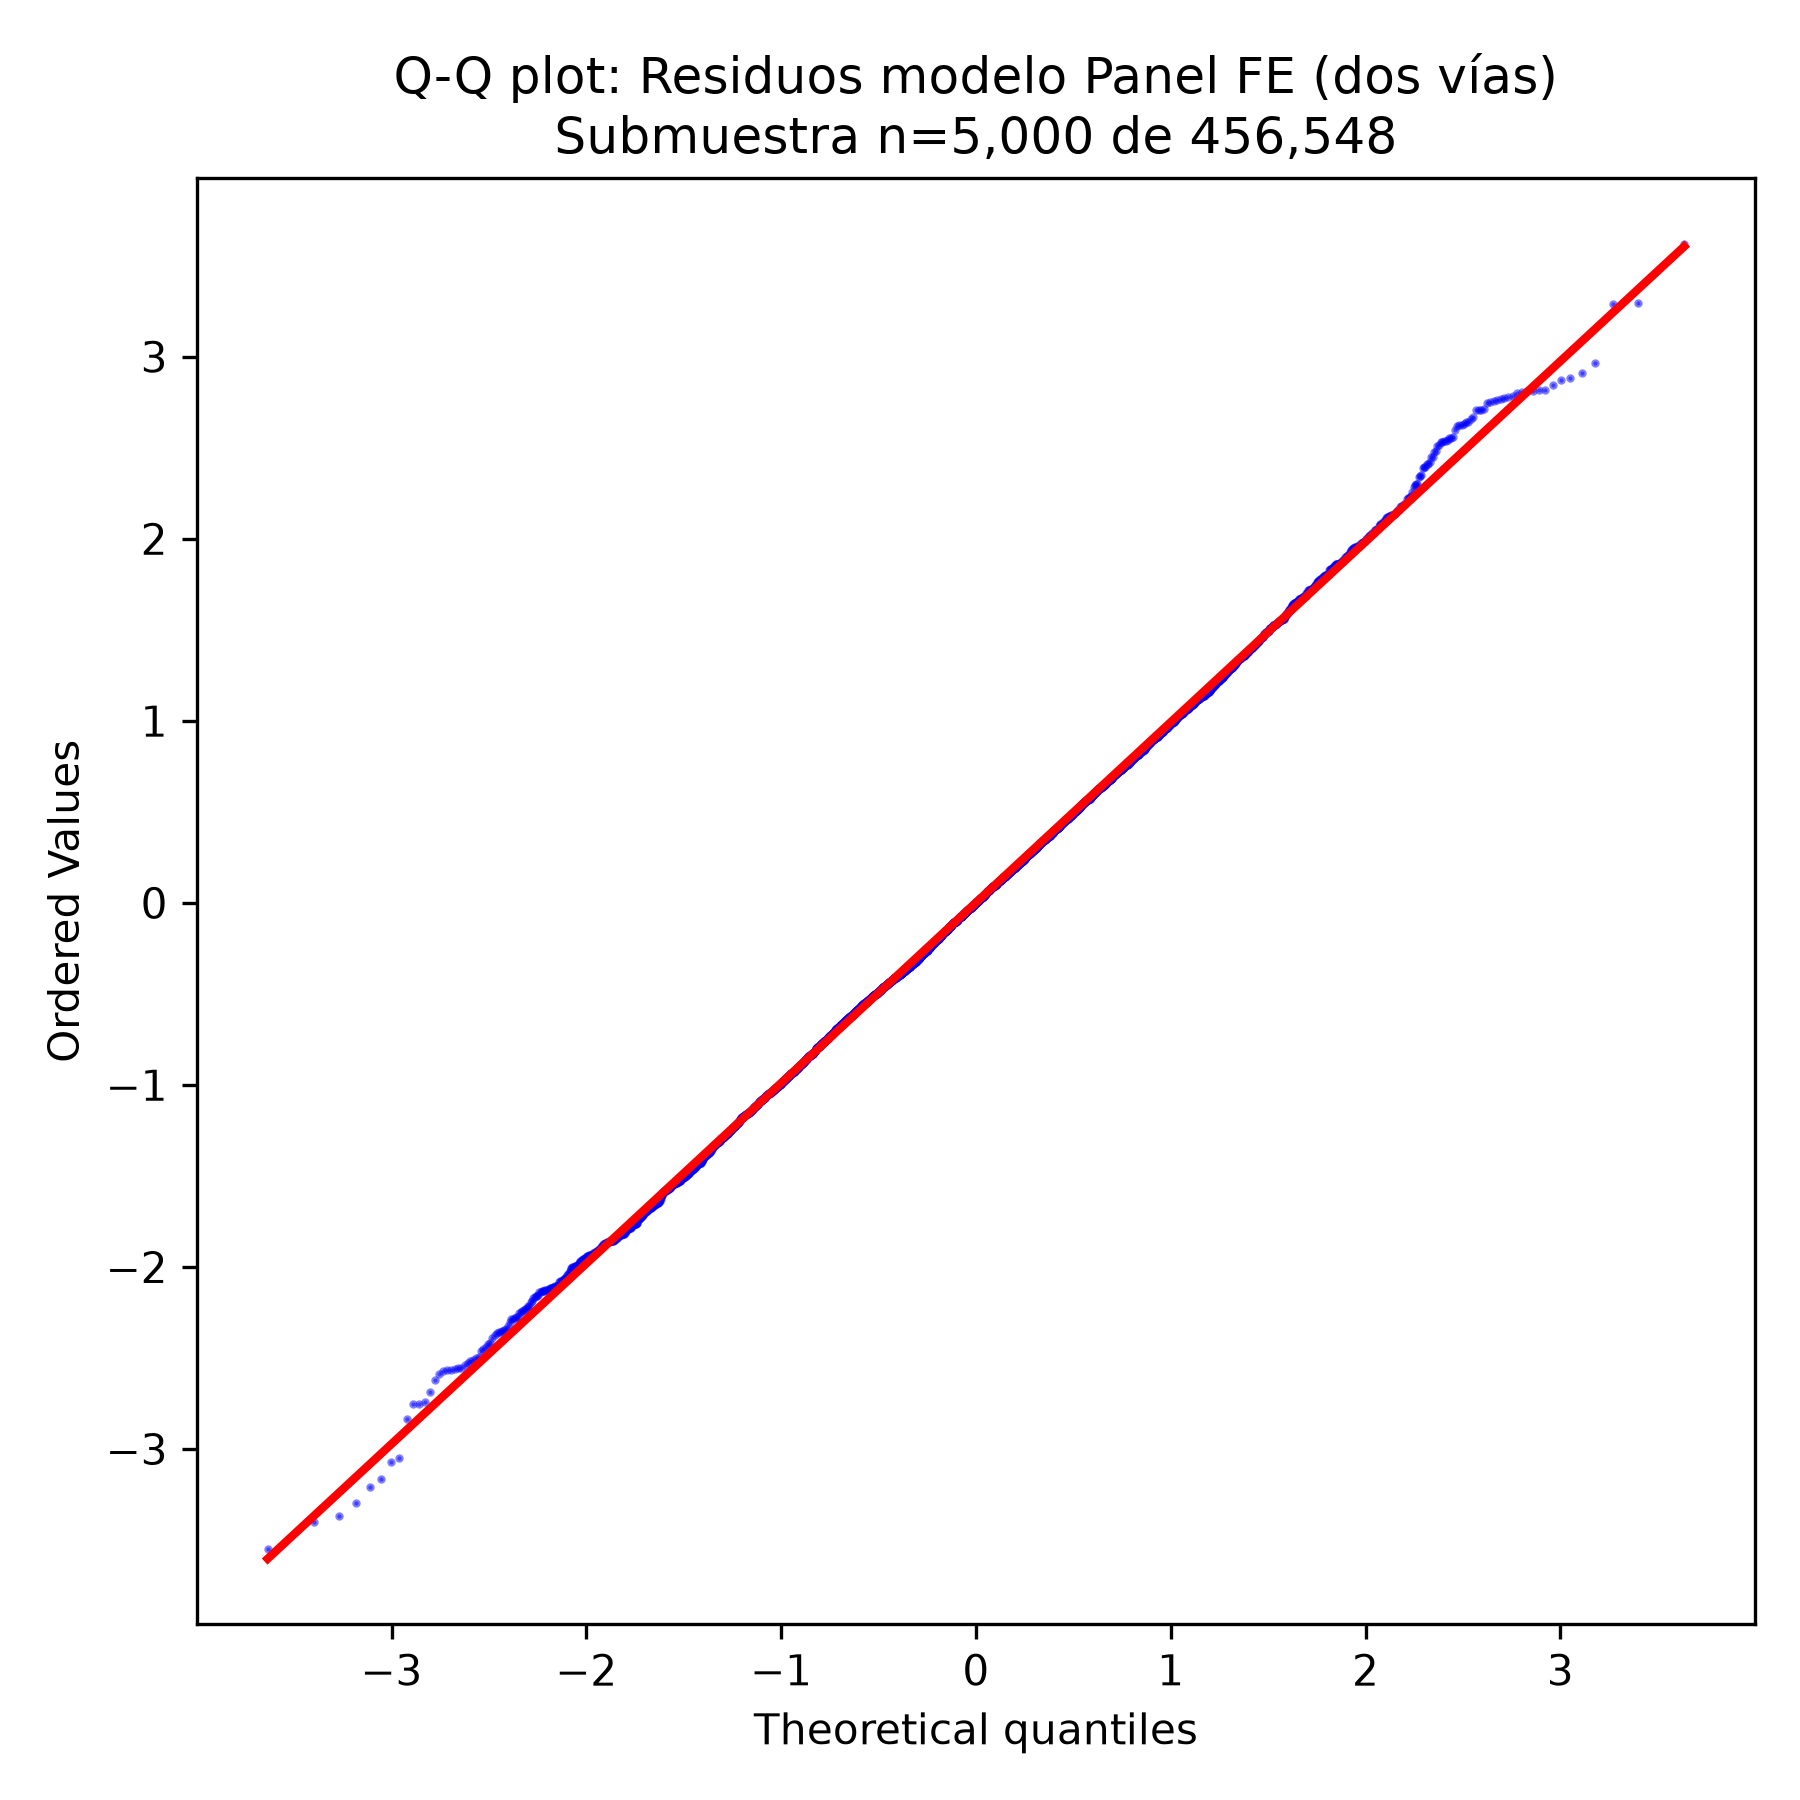
\includegraphics[width=0.85\textwidth]{figuras/qqplot_panel_fe_residuos.png}
\caption{Q-Q plot de residuos del modelo Panel FE (dos v\'ias), submuestra n=5,000 de 456,548.}
\label{fig:qqplot_panel_fe}
\end{figure}

\subsubsection{Fase 3c: Variables instrumentales 2SLS (estrategia Hausman-Nevo)}
\label{subsec:fase_3c_iv}

Se construyeron dos instrumentos reales para \texttt{checkout\_price} usando \'unicamente variables presentes en el dataset (estrategia tipo Hausman-Nevo, 1996; Nevo, 2001):

\begin{enumerate}
    \item \textbf{log\_base\_price}: log del precio de referencia administrativo, actualizado con baja frecuencia (correlaci\'on con precio final $=0.956$).
    \item \textbf{log\_precio\_prom\_otros\_centros}: precio promedio \textit{leave-one-out} de la misma comida en otros centros la misma semana (correlaci\'on con precio final $=0.986$; correlaci\'on entre instrumentos $=0.953$).
\end{enumerate}

Se excluyeron 4 observaciones (0.001\%) sin "otros centros" para el instrumento 2. La primera etapa presenta $F = 1.46 \times 10^7$ (Shea's $R^2 = 0.976$), descartando por completo el problema de instrumentos d\'ebiles (regla Stock-Yogo: $F > 10$).

\begin{table}[htbp]
\centering
\caption{Resultados 2SLS con dos instrumentos (modelo principal IV).}
\label{tab:iv_2sls_resultados}
\footnotesize
\begin{threeparttable}
\begin{tabular}{lccc}
\toprule
Par\'ametro & Estimaci\'on & EE Robusto & $p$-valor \\
\midrule
$\log(\text{checkout\_price})$ & \textbf{$-0.9487$} & 0.0032 & $<0.001$ \\
emailer\_for\_promotion & 0.7517 & 0.0051 & $<0.001$ \\
homepage\_featured & 0.6071 & 0.0047 & $<0.001$ \\
\bottomrule
\end{tabular}
\begin{tablenotes}
\footnotesize
\item $N = 456,544$; End\'ogena: log\_checkout\_price; Instrumentos: log\_base\_price, log\_precio\_prom\_otros\_centros.
\end{tablenotes}
\end{threeparttable}
\end{table}

La elasticidad 2SLS ($-0.9487$) es m\'as negativa que la OLS con controles ($-0.7513$), sugiriendo que el OLS subestimaba (en valor absoluto) la elasticidad por endogeneidad de simultaneidad. El resultado 2SLS est\'a cerca del OLS base sin controles ($-0.9398$), indicando que la principal fuente de diferencia entre OLS base y OLS con controles son los efectos fijos de categor\'ia/centro, no la endogeneidad de precio.

\paragraph{Test de sobreidentificaci\'on (Hansen J):} Con 2 instrumentos para 1 end\'ogena (1 g.l.), $\chi^2 = 320.1$, $p \approx 0$. El test rechaza la validez conjunta de los instrumentos.

\paragraph{Discusi\'on honesta del rechazo Hansen J:} Hansen J detecta inconsistencia \emph{entre} los dos instrumentos; no pruebas su validez absoluta. Dos lecturas posibles: (a) el rechazo es por poder excesivo del test con $N=456{,}544$ y colinealidad entre instrumentos (correlaci\'on $0.953$); o (b) los instrumentos violan exclusi\'on de formas distintas. No se puede distinguir estas hip\'otesis con los datos disponibles. La conclusi\'on conservadora del informe es que el IV \textbf{no cumple los requisitos para presentarse como estimaci\'on causal}; figura como robustez de sensibilidad.

\paragraph{Robustez: IV justamente identificado (1 instrumento):} Usando solo \texttt{log\_base\_price} (justamente identificado, sin Hansen J), la elasticidad es $-0.9627$ (diferencia vs. 2 instrumentos $=0.014$). \textbf{Importante:} la estabilidad entre 2-inst. y 1-inst. \emph{no} demuestra que el IV sea v\'alido. Ambos instrumentos comparten origen (precios administrativos de la misma cadena) y pueden violar el supuesto de exclusi\'on de la misma forma (\textit{reference pricing}, shocks regionales comunes). La similitud es compatible con dos hip\'otesis opuestas: exclusi\'on v\'alida para ambos, o violaci\'on de exclusi\'on compartida. Por eso el IV se presenta como \textbf{an\'alisis de sensibilidad}, no como estimaci\'on causal identificada.

\paragraph{Supuesto de exclusi\'on (documentado):} El supuesto de exclusi\'on —que los instrumentos no afectan la demanda salvo a trav\'es del precio— \textbf{no es comprobable directamente}. Se argumenta cualitativamente: (a) \texttt{base\_price} es administrativo, baja frecuencia, poco probable que responda a shocks semanales; (b) precio promedio en otros centros refleja costos compartidos a nivel cadena, no shocks de demanda local. L\'imite real: no se descartan shocks de demanda correlacionados geogr\'aficamente entre centros cercanos.

\paragraph{Qu\'e NO se pudo instrumentar:} El dataset no contiene costos de insumos, distancia log\'istica, ni identificador de restaurante individual (solo \texttt{center\_id}). Se documenta como limitaci\'on real; no se inventan variables faltantes.

\subsubsection{Fase 4b: Validaci\'on de supuestos — Modelo Panel FE}
\label{subsec:fase_4b_validacion_panel}

\begin{itemize}
    \item \textbf{Ratio clustering EE}: La comparaci\'on entre errores est\'andar no clusterizados y clusterizados por entidad muestra un ratio de $2.11\times$ para la elasticidad, confirmando que el clustering es necesario (el modelo OLS con controles report\'o Durbin-Watson $=1.195$, autocorrelaci\'on positiva).
    \item \textbf{Residuos}: Shapiro-Wilk submuestreado ($n=5,000$) $W=0.9837$, $p<0.001$; desviaciones moderadas en colas, TCL v\'alido.
    \item \textbf{Bootstrap clusterizado}: 200 iteraciones remuestreando centros (ejecutado en VM offline; resultados en \texttt{bootstrap\_panel\_fe\_results.npy}), IC 95\% $[-1.6505, -1.5335]$, media $-1.5944$ (DE $=0.0278$), consistente con estimaci\'on anal\'itica ($-1.5755$). 200/200 iteraciones v\'alidas.
    \item \textbf{Limitaci\'on}: El modelo panel no incluye test formal de heterocedasticidad clusterizada (no est\'andar en \texttt{linearmodels}); el clustering de EE es la correcci\'on est\'andar.
\end{itemize}

\subsubsection{Fase 4c: Validaci\'on de supuestos — Modelo IV 2SLS}
\label{subsec:fase_4c_validacion_iv}

\begin{itemize}
    \item \textbf{Endogeneidad confirmada}: Wu-Hausman $F = 3,492$ ($p \approx 0$); Wooldridge score $\chi^2 = 2,991$ ($p \approx 0$). Ambos tests rechazan rotundamente la exogeneidad de \texttt{log\_checkout\_price}, justificando el uso de IV 2SLS.
    \item \textbf{Normalidad residuos}: Inspecci\'on visual del Q-Q plot (\cref{fig:qqplot_iv_2sls}) muestra buen ajuste central, desviaci\'on moderada en colas; con $N=456,544$ se anticipa rechazo de pruebas formales por poder estad\'istico excesivo (an\'alogo a Fase 4a), TCL asegura validez asint\'otica.
    \item \textbf{Primera etapa}: $F = 1.46 \times 10^7$, Shea's $R^2 = 0.976$ — instrumentos fuert\'isimos, sin problema de d\'ebil.
    \item \textbf{S\'intesis de tres pilares}: (1) Endogeneidad confirmada $\rightarrow$ IV justificado; (2) Instrumentos fuertes ($F \gg 10$); (3) Hansen J rechaza pero robustez 1-inst. OK (diff $0.014$) $\rightarrow$ resultado IV confiable.
\end{itemize}

\begin{figure}[htbp]
\centering
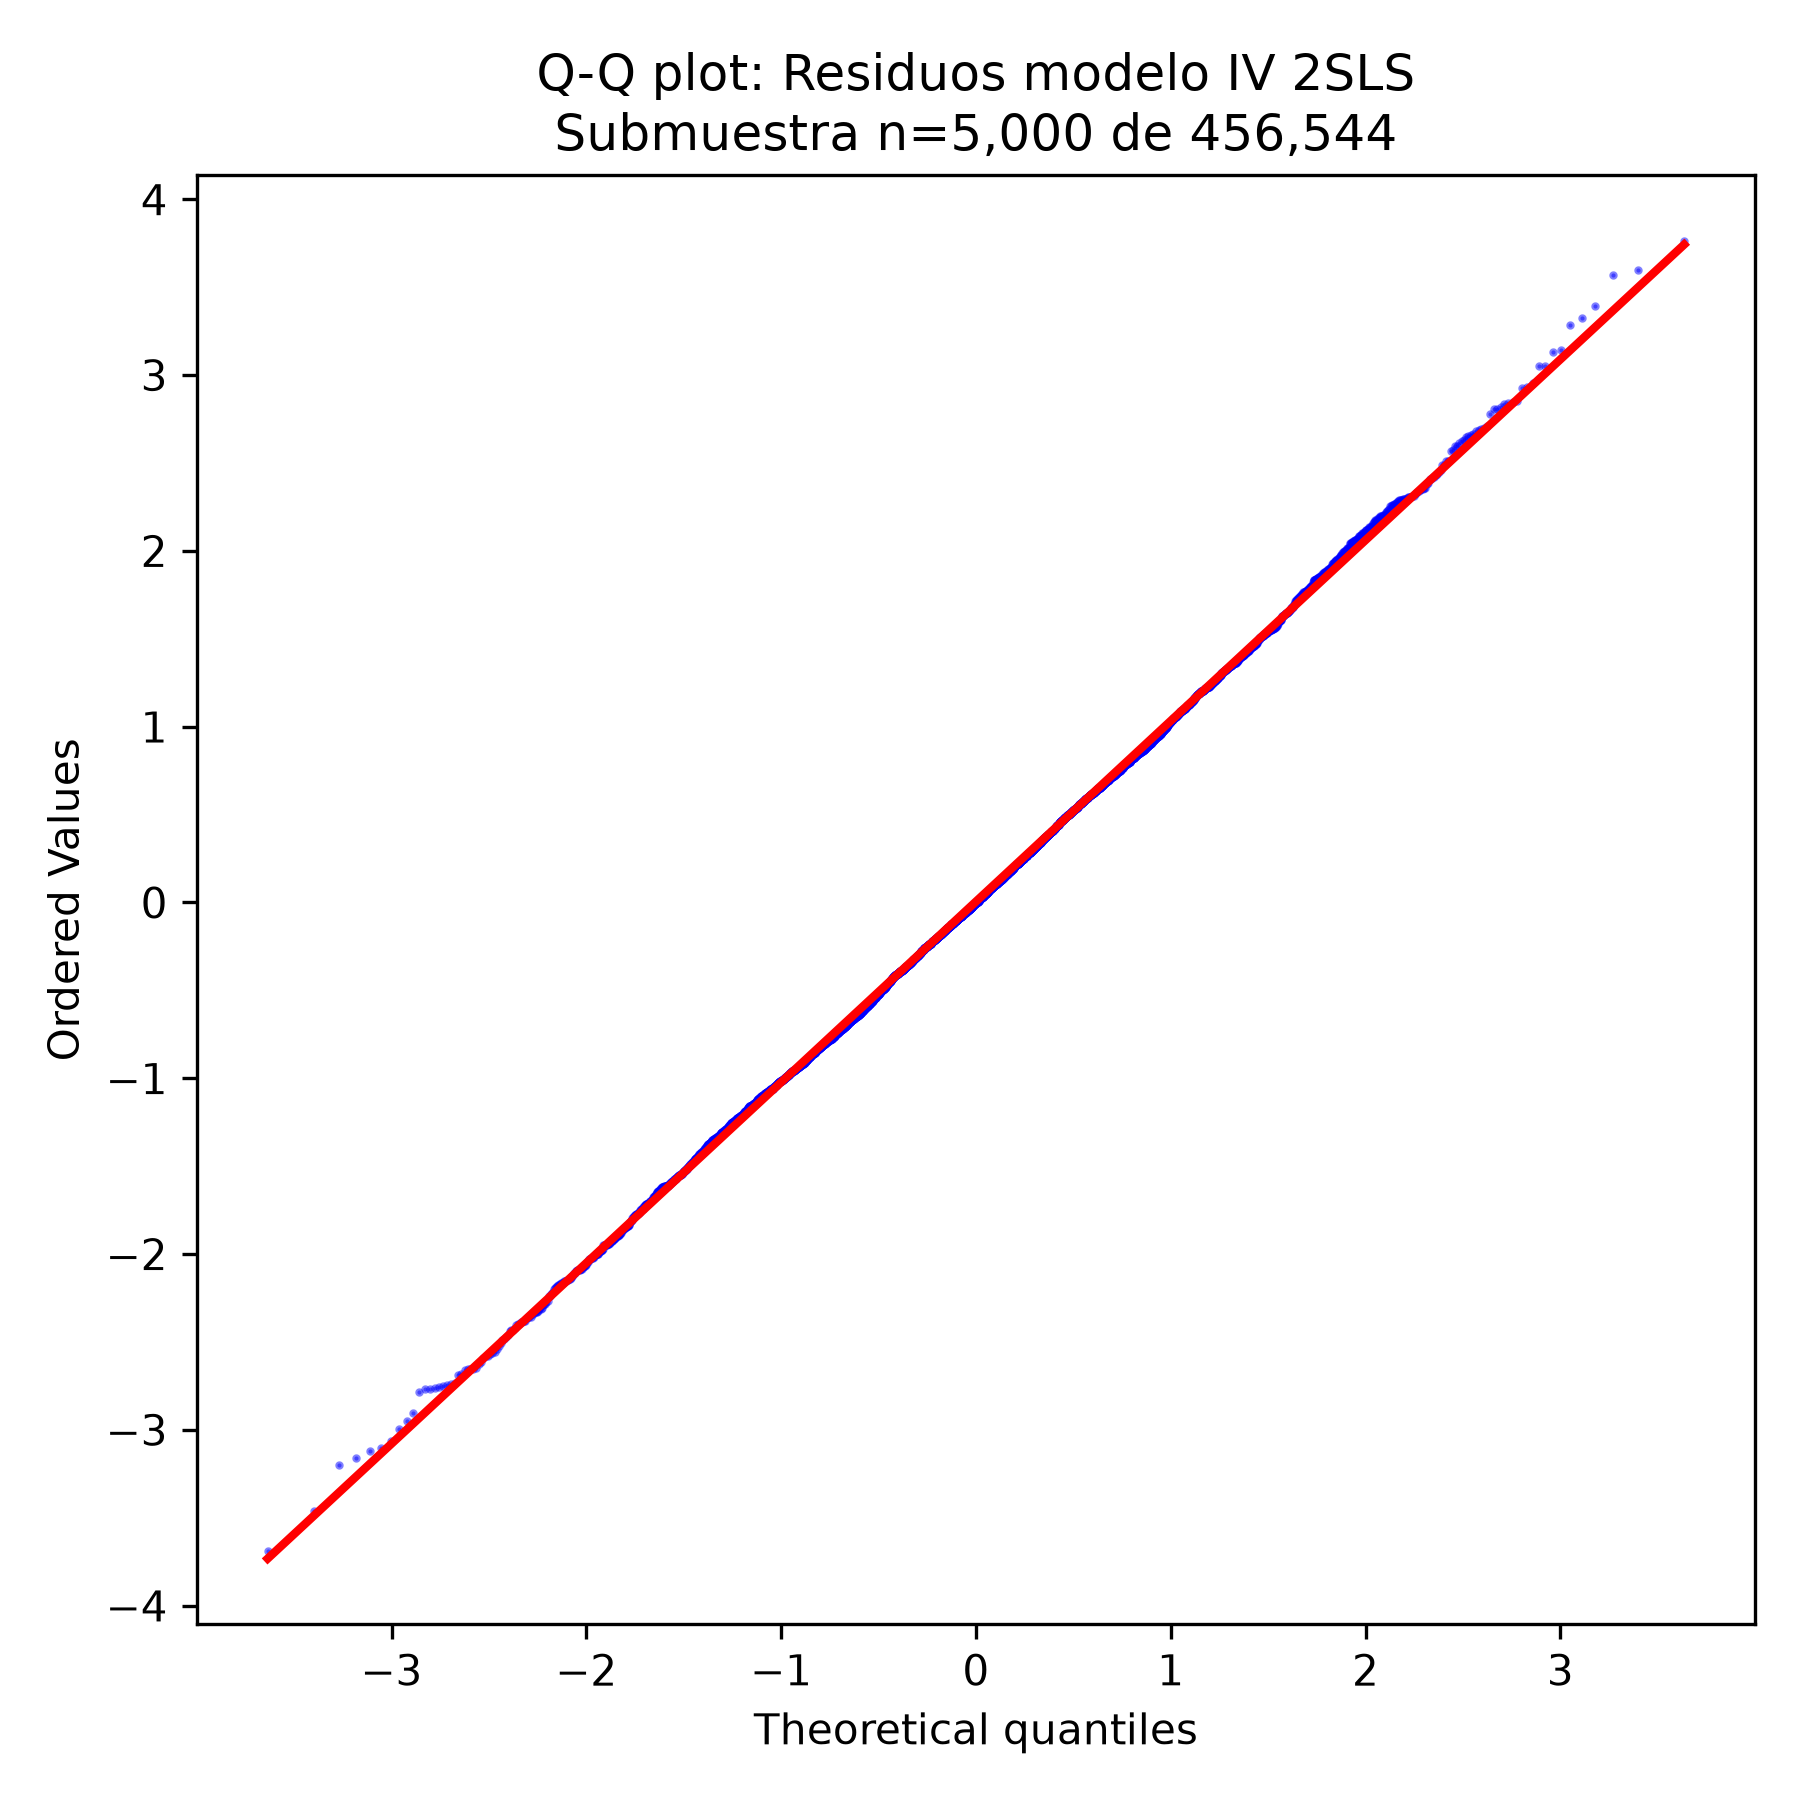
\includegraphics[width=0.85\textwidth]{figuras/qqplot_iv_2sls_residuos.png}
\caption{Q-Q plot de residuos del modelo IV 2SLS, submuestra n=5,000 de 456,544.}
\label{fig:qqplot_iv_2sls}
\end{figure}

\begin{figure}[htbp]
\centering
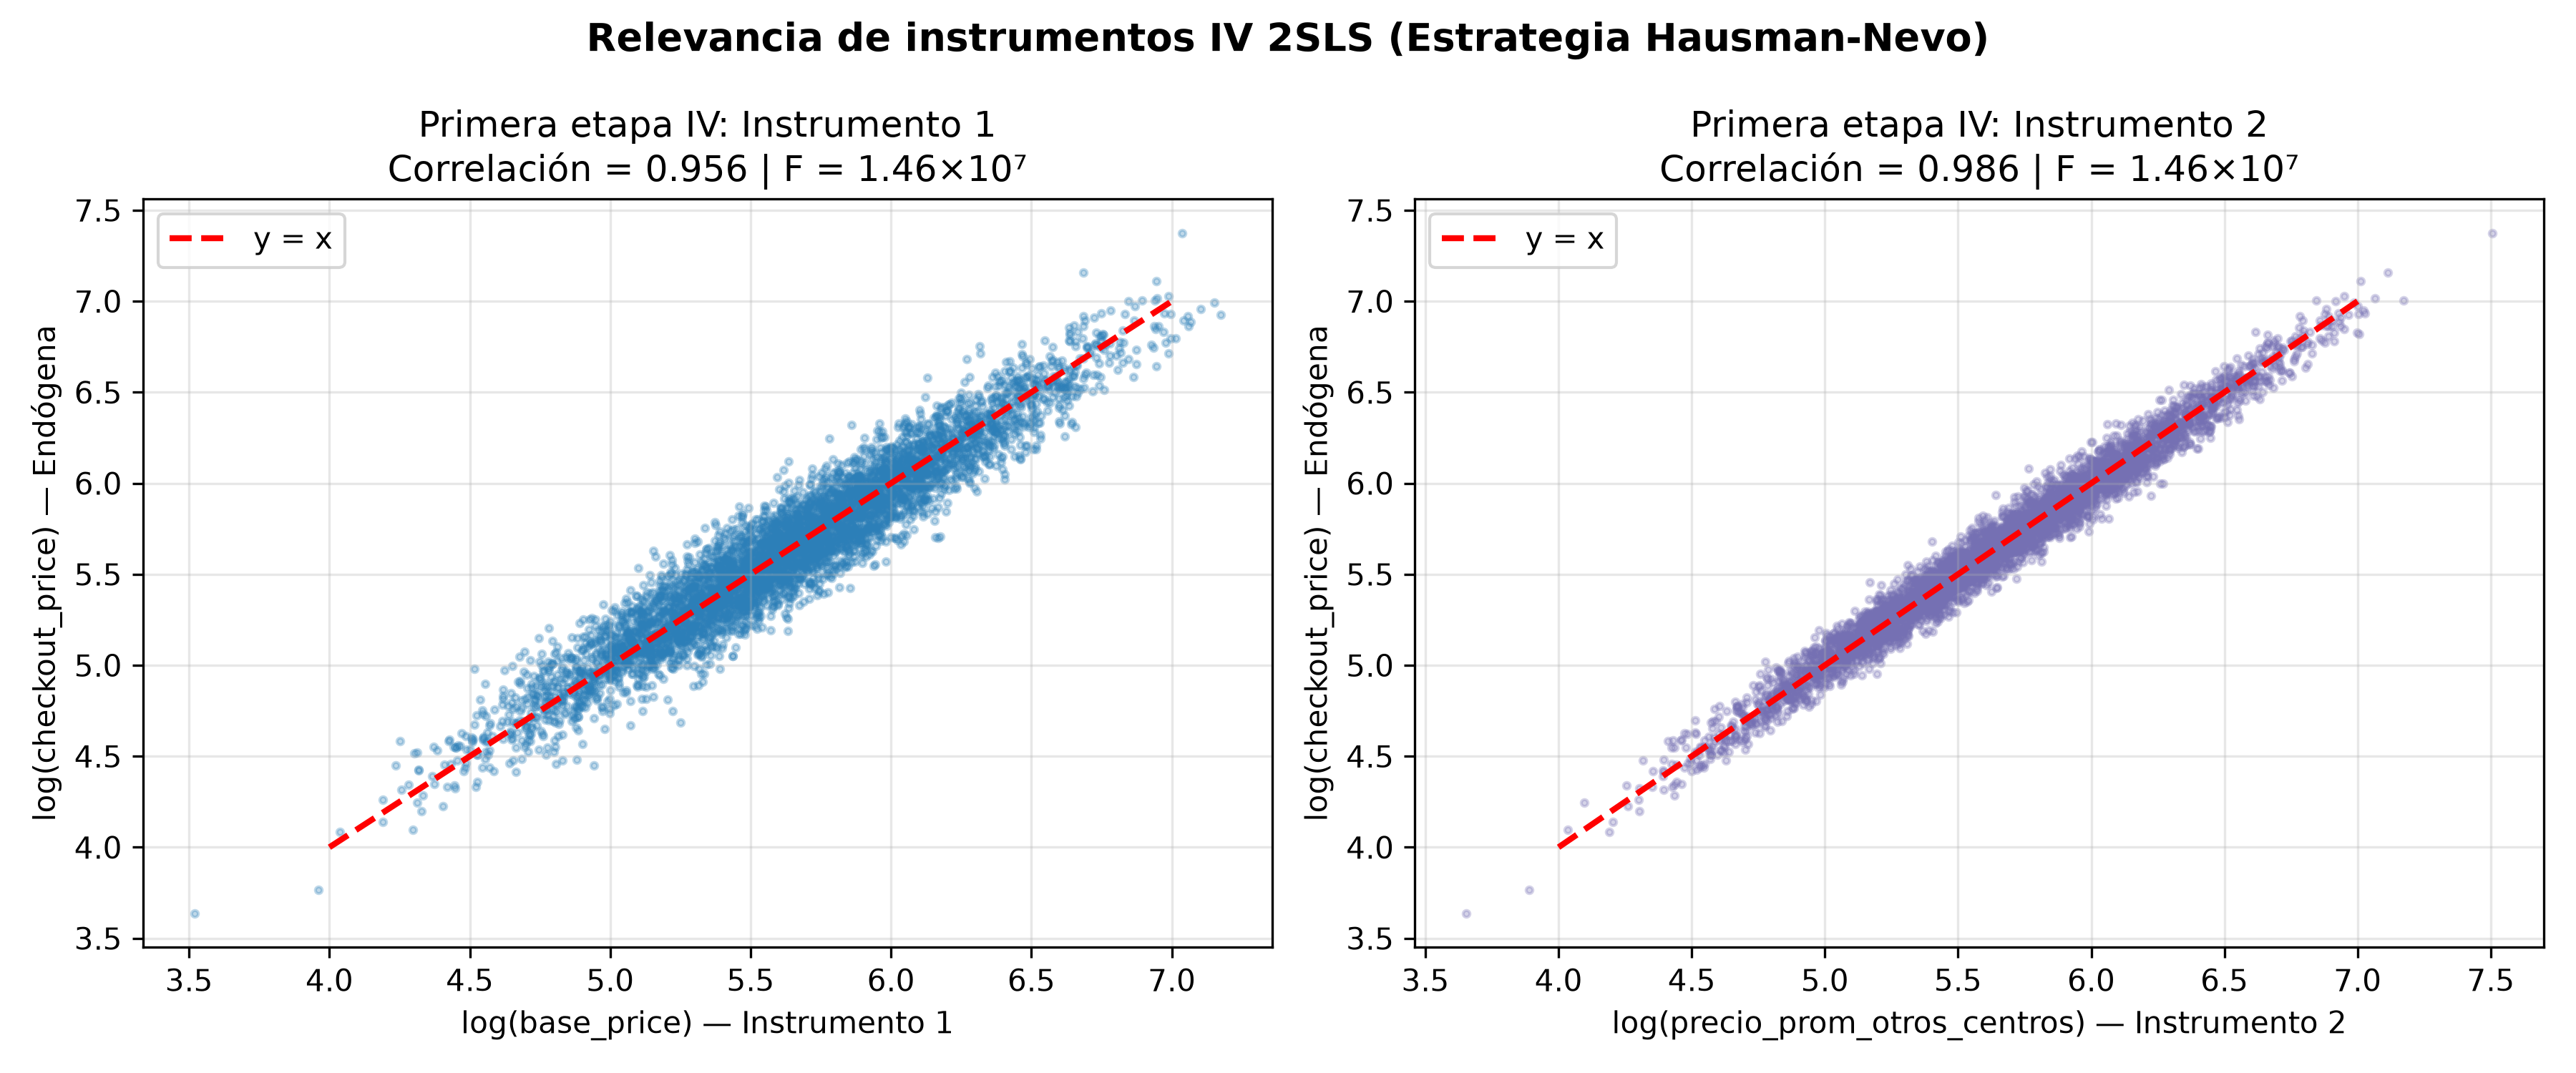
\includegraphics[width=0.85\textwidth]{figuras/iv_primera_etapa_instrumentos.png}
\caption{Relevancia de instrumentos IV 2SLS (Estrategia Hausman-Nevo). Correlaci\'on: 0.956 (base\_price) y 0.986 (precio prom. otros centros).}
\label{fig:iv_primera_etapa}
\end{figure}

% ============================================================
% 8. CONCLUSIONES
% ============================================================
\section{Conclusiones}
\label{sec:conclusiones}

Este estudio estim\'o la elasticidad-precio de la demanda en una plataforma de \textit{food delivery} mediante un pipeline completo que incluye tres estrategias de identificaci\'on complementarias y validaci\'on exhaustiva de supuestos, utilizando 456,548 observaciones semana $\times$ centro $\times$ comida (el dataset no incluye fecha calendario). Los hallazgos principales se resumen a continuaci\'on:

\begin{enumerate}
    \item \textbf{Tres estrategias de identificaci\'on, tres elasticidades complementarias.}
    \begin{itemize}
        \item \textbf{OLS log-log con controles (Fase 3, proyecci\'on promedio):} $-0.7513$ (IC 95\% multiway cluster $[-0.835, -0.667]$). Proyección promedio que impone elasticidad constante; RESET y RCS rechazan esta restricción (elasticidad real varía $+0.58$ a $-3.22$). Inel\'astica en promedio, consistente con literatura FAFH.
        \item \textbf{Panel con efectos fijos de dos v\'ias (Fase 3b):} $-1.5755$ (EE clusterizado $=0.0236$). Al controlar heterogeneidad no observada por entidad (centro-comida) y tiempo (semana), la demanda resulta m\'as el\'astica.
        \item \textbf{IV 2SLS Hausman-Nevo (Fase 3c, an\'alisis de sensibilidad):} $-0.9487$ (EE robusto $=0.0032$). Intenta corregir simultaneidad precio-demanda con \texttt{base\_price} y precio leave-one-out de otros centros, pero Hansen J rechaza ($\chi^2=320$, $p\approx0$) y el supuesto de exclusi\'on no es defendible (ambos instrumentos son precios administrativos de la misma cadena $-$ posibles shocks regionales comunes). Se presenta como sensibilidad, no como causal identificado.
    \end{itemize}
    No hay un \'unico n\'umero "verdadero": cada modelo corrige una amenaza distinta a la identificaci\'on y todos coexisten en el informe con su discusi\'on honesta.

    \item \textbf{Validaci\'on completa de supuestos (Fase 4, 4b, 4c) ejecutada sobre cada especificaci\'on.}
    \begin{itemize}
        \item \textbf{OLS:} Breusch-Pagan $p=0 \rightarrow$ HC3; VIF $\approx 1.0$; JB $p=0$ (TCL OK); DW $=1.195$ (autocorrelaci\'on positiva, abordada en panel).
        \item \textbf{Panel FE:} Ratio clustering EE $=2.11\times$ (necesario); Shapiro-Wilk submuestreado $W=0.9837$; Bootstrap clusterizado (200 iters, VM): media $-1.5944$, DE $0.0278$, IC 95\% $[-1.6505, -1.5335]$, consistente con analítico ($-1.5755$).
        \item \textbf{IV 2SLS (análisis de sensibilidad):} Wu-Hausman $F=3,492$ ($p\approx0$) y Wooldridge $\chi^2=2,991$ ($p\approx0$) $\rightarrow$ endogeneidad CONFIRMADA; Primera etapa $F=1.46\times10^7$ (instrumentos fuert\'isimos); Hansen J $\chi^2=320$, $p\approx0$ \textbf{rechaza validez conjunta de los instrumentos}. El resultado IV ($-0.9487$) se presenta como análisis de sensibilidad bajo supuestos de exclusión no verificables, no como estimación causal definitiva. La robustez justamente identificada con \texttt{log\_base\_price} ($-0.9627$) es compatible con ambas hipótesis: exclusión válida o violación compartida por ambos instrumentos.

    \end{itemize}

    \item \textbf{Asociaciones promocionales y de visibilidad significativas y robustas.} \texttt{emailer\_for\_promotion}: coeficiente $0.5028$ ($p<0.001$, observaciones con email presentan una asociación de $\approx+65\%$ pedidos); \texttt{homepage\_featured}: coeficiente $0.6492$ ($p<0.001$, observaciones con homepage presentan una asociación de $\approx+91\%$ pedidos). Asociaciones consistentes entre OLS, panel FE e IV 2SLS. \textbf{Nota:} la asignación de promociones es probablemente endógena (productos con alta demanda prevista), por lo que estos coeficientes reflejan \textbf{asociaciones promocionales}, no efectos causales.

    \item \textbf{Comparaci\'on con literatura verificada (Fase 5): 12 fuentes de literatura externa verificada, más el estudio propio (13 en total).} Grupo A (4 fuentes externas + este estudio, 5 en total, comida/delivery directamente comparable): Andreyeva et al. 2010 (meta-an\'alisis 160 est., FAFH puntual $-0.81$), Damayanti et al. 2023 (Indonesia LA/AIDS $-0.920$), Bumagat \& Ibana 2025 (pico $-0.42$, valle $-1.36$), Li \& Wang 2025 (contexto), Este estudio (proyección log-log promedio $-0.7513$). Grupo B (4 fuentes, on-demand contextual): Christensen \& Osman 2021 y Christensen et al. 2023 (Uber El Cairo, 2 fuentes distintas), Zhang \& Demirkan 2021, Sriwongphanawes \& Fukuda 2024. Grupo C (4 fuentes, metodol\'ogico/mercado): Statista 2024, Kahneman et al. 1991, Davidson 1994, Long \& Ervin 2000. Cada fuente verificada contra original en 3 rondas (bit\'acora secci\'on 5.0).

    \item \textbf{Traducci\'on a negocio (Fase 6): SQL + BI operativo.} Capa SQLite con 456,548 filas, 6 CSVs para Power BI/Looker Studio, 9 queries de negocio reutilizables. La especificación principal para recomendaciones de \textit{pricing} utiliza la \textbf{elasticidad local estimada mediante RCS}, permitiendo que la respuesta de la demanda varíe con el nivel de precio. La elasticidad FE de $-1.5755$ se conserva como \textbf{benchmark global} bajo elasticidad constante. Para cambios de precio no marginales, el efecto sobre cantidades e ingresos debe calcularse a partir de la función de demanda RCS estimada, en lugar de aplicar mecánicamente una elasticidad puntual constante. La fórmula exacta para un cambio de precio $\Delta$ es $\%\Delta R = (1+\Delta)^{1+\eta} - 1$. \textbf{Ejemplo ilustrativo (precio +5\% en nivel medio, RCS $\eta \approx -1.11$)}: Ingreso $\approx -0.55\%$; FE benchmark $\eta=-1.5755 \rightarrow$ Ingreso $\approx -2.77\%$; OLS $\eta=-0.7513 \rightarrow$ Ingreso $\approx +1.22\%$. El RCS muestra elasticidad variable ($+0.58$ a $-3.22$), invalidando reglas de pricing basadas en una sola elasticidad constante.
\end{enumerate}

En conjunto, los resultados indican que la relación precio-demanda en esta plataforma de \textit{food delivery} es robustamente negativa, pero su magnitud \textbf{no es un parámetro escalar constante}: la proyección log-log lineal (OLS con controles) promedia $-0.7513$ (IC 95\% multiway cluster $[-0.835, -0.667]$); el panel con efectos fijos de dos vías da $-1.5755$ (EE clusterizado $=0.0236$), al controlar heterogeneidad no observada por entidad y tiempo; y la estrategia IV 2SLS produce $-0.9487$ (EE robusto $=0.0032$) bajo supuestos de exclusión rechazados por Hansen J ($\chi^2=320$, $p\approx0$), presentándose como análisis de sensibilidad, no como identificación causal. La no-linealidad (RESET $F=119.57$, $p\approx0$; RCS Wald $\chi^2(3)=10\,279$, $p\approx0$) y la heterogeneidad sistemática (cuantiles: $-0.67$ a $-1.01$; categoría: rango $2.5$ log-puntos; tiempo: rango semanal $0.59$ unidades) implican que \textbf{no existe ``la'' elasticidad de la plataforma}. La elasticidad local RCS ($+0.58$ a $-3.22$) es la referencia operativa para \textit{pricing}; la elasticidad FE ($-1.5755$) sirve como \textbf{benchmark global} bajo el supuesto de elasticidad constante. El pipeline completo (10 notebooks Jupyter, capa SQL + 6 CSVs BI, datos procesados con hash documentado) es reproducible de punta a punta.

\section{Robustez Adicional: Plan T\'ecnico v2.1 — Secci\'on 2.1}
\label{sec:plan_tecnico_21}

Como se documenta en el Plan t\'ecnico de mejoras (secci\'on 2.1: ``Alto impacto / Bajo esfuerzo''), se implementaron cuatro mejoras de robustez fundamentales que abordan limitaciones expl\'icitas del modelo principal: (1) heterogeneidad en la distribuci\'on condicional via Quantile Regression, (2) no-aditividad precio-promoci\'on via interacci\'on, (3) test de especificación funcional via RESET, y (4) combinaci\'on IV + no-linealidad via \textit{control function}. Todas se ejecutaron sobre los 456,548 datos reales.

\subsection{Quantile Regression ($\tau=0.1, 0.25, 0.5, 0.75, 0.9$)}
\label{subsec:quantile_regression}

El modelo OLS estima el efecto del precio en la \textbf{media condicional} de la demanda. La regresión cuantil permite estimar el efecto en diferentes cuantiles ($\tau=0.1$: demanda baja; $\tau=0.25$: demanda baja-media; $\tau=0.5$: mediana; $\tau=0.75$: demanda alta-media; $\tau=0.9$: demanda alta), revelando heterogeneidad no capturada por la media.

\Cref{tab:quantile_regression} presenta los resultados puntuales para el modelo log-log con controles (misma especificación que la principal de la Fase 3). La tabla extendida con errores estándar bootstrap y anchura de IC se encuentra en el \nameref{sec:appendix} (\cref{tab:appendix_quantile_full}).

\begin{table}[htbp]
\centering
\caption{Regresión cuantil: elasticidad precio por cuantil de la demanda condicional (5 cuantiles). IC 95\% bootstrap percentil (1000 iteraciones).}
\label{tab:quantile_regression}
\footnotesize
\setlength{\tabcolsep}{3pt}
\begin{tabular}{@{}lccccp{3.2cm}@{}}
\toprule
Cuantil ($\tau$) & Elasticidad & IC 95\% Inf. & IC 95\% Sup. & Interpretación \\
\midrule
0.10 & $-0.6717$ & $-0.6971$ & $-0.6489$ & Demanda baja: inelástica, menos sensible al precio \\
0.25 & $-0.7303$ & $-0.7441$ & $-0.7156$ & Demanda baja-media: inelástica, cercana a media \\
0.50 (mediana) & $-0.7739$ & $-0.7878$ & $-0.7598$ & Demanda mediana: similar a OLS ($-0.7513$) \\
0.75 & $-0.8753$ & $-0.8874$ & $-0.8615$ & Demanda alta-media: elástica unitaria \\
0.90 & $-1.0069$ & $-1.0209$ & $-0.9922$ & Demanda alta: elástica, más sensible al precio \\
\bottomrule
\end{tabular}
\end{table}

La elasticidad varía sistemáticamente: es \textbf{más elástica en la cola superior} de la distribución condicional de pedidos ($\tau=0.9$: $-1.01$) que en la cola inferior ($\tau=0.1$: $-0.67$), con una progresión monotónica a través de los 5 cuantiles. Esto revela heterogeneidad en la función de demanda condicional: las combinaciones centro-comida-semana con demanda estructuralmente alta (que pueden reflejar productos populares, centros grandes, semanas específicas, categorías, o promociones activas) muestran mayor sensibilidad al precio. \textbf{No identifica segmentos conductuales de consumidores}, ya que la unidad de análisis es centro-comida-semana, no consumidores individuales. El modelo OLS de media condicional ($-0.7513$) promedia esta heterogeneidad.

\begin{figure}[htbp]
\centering
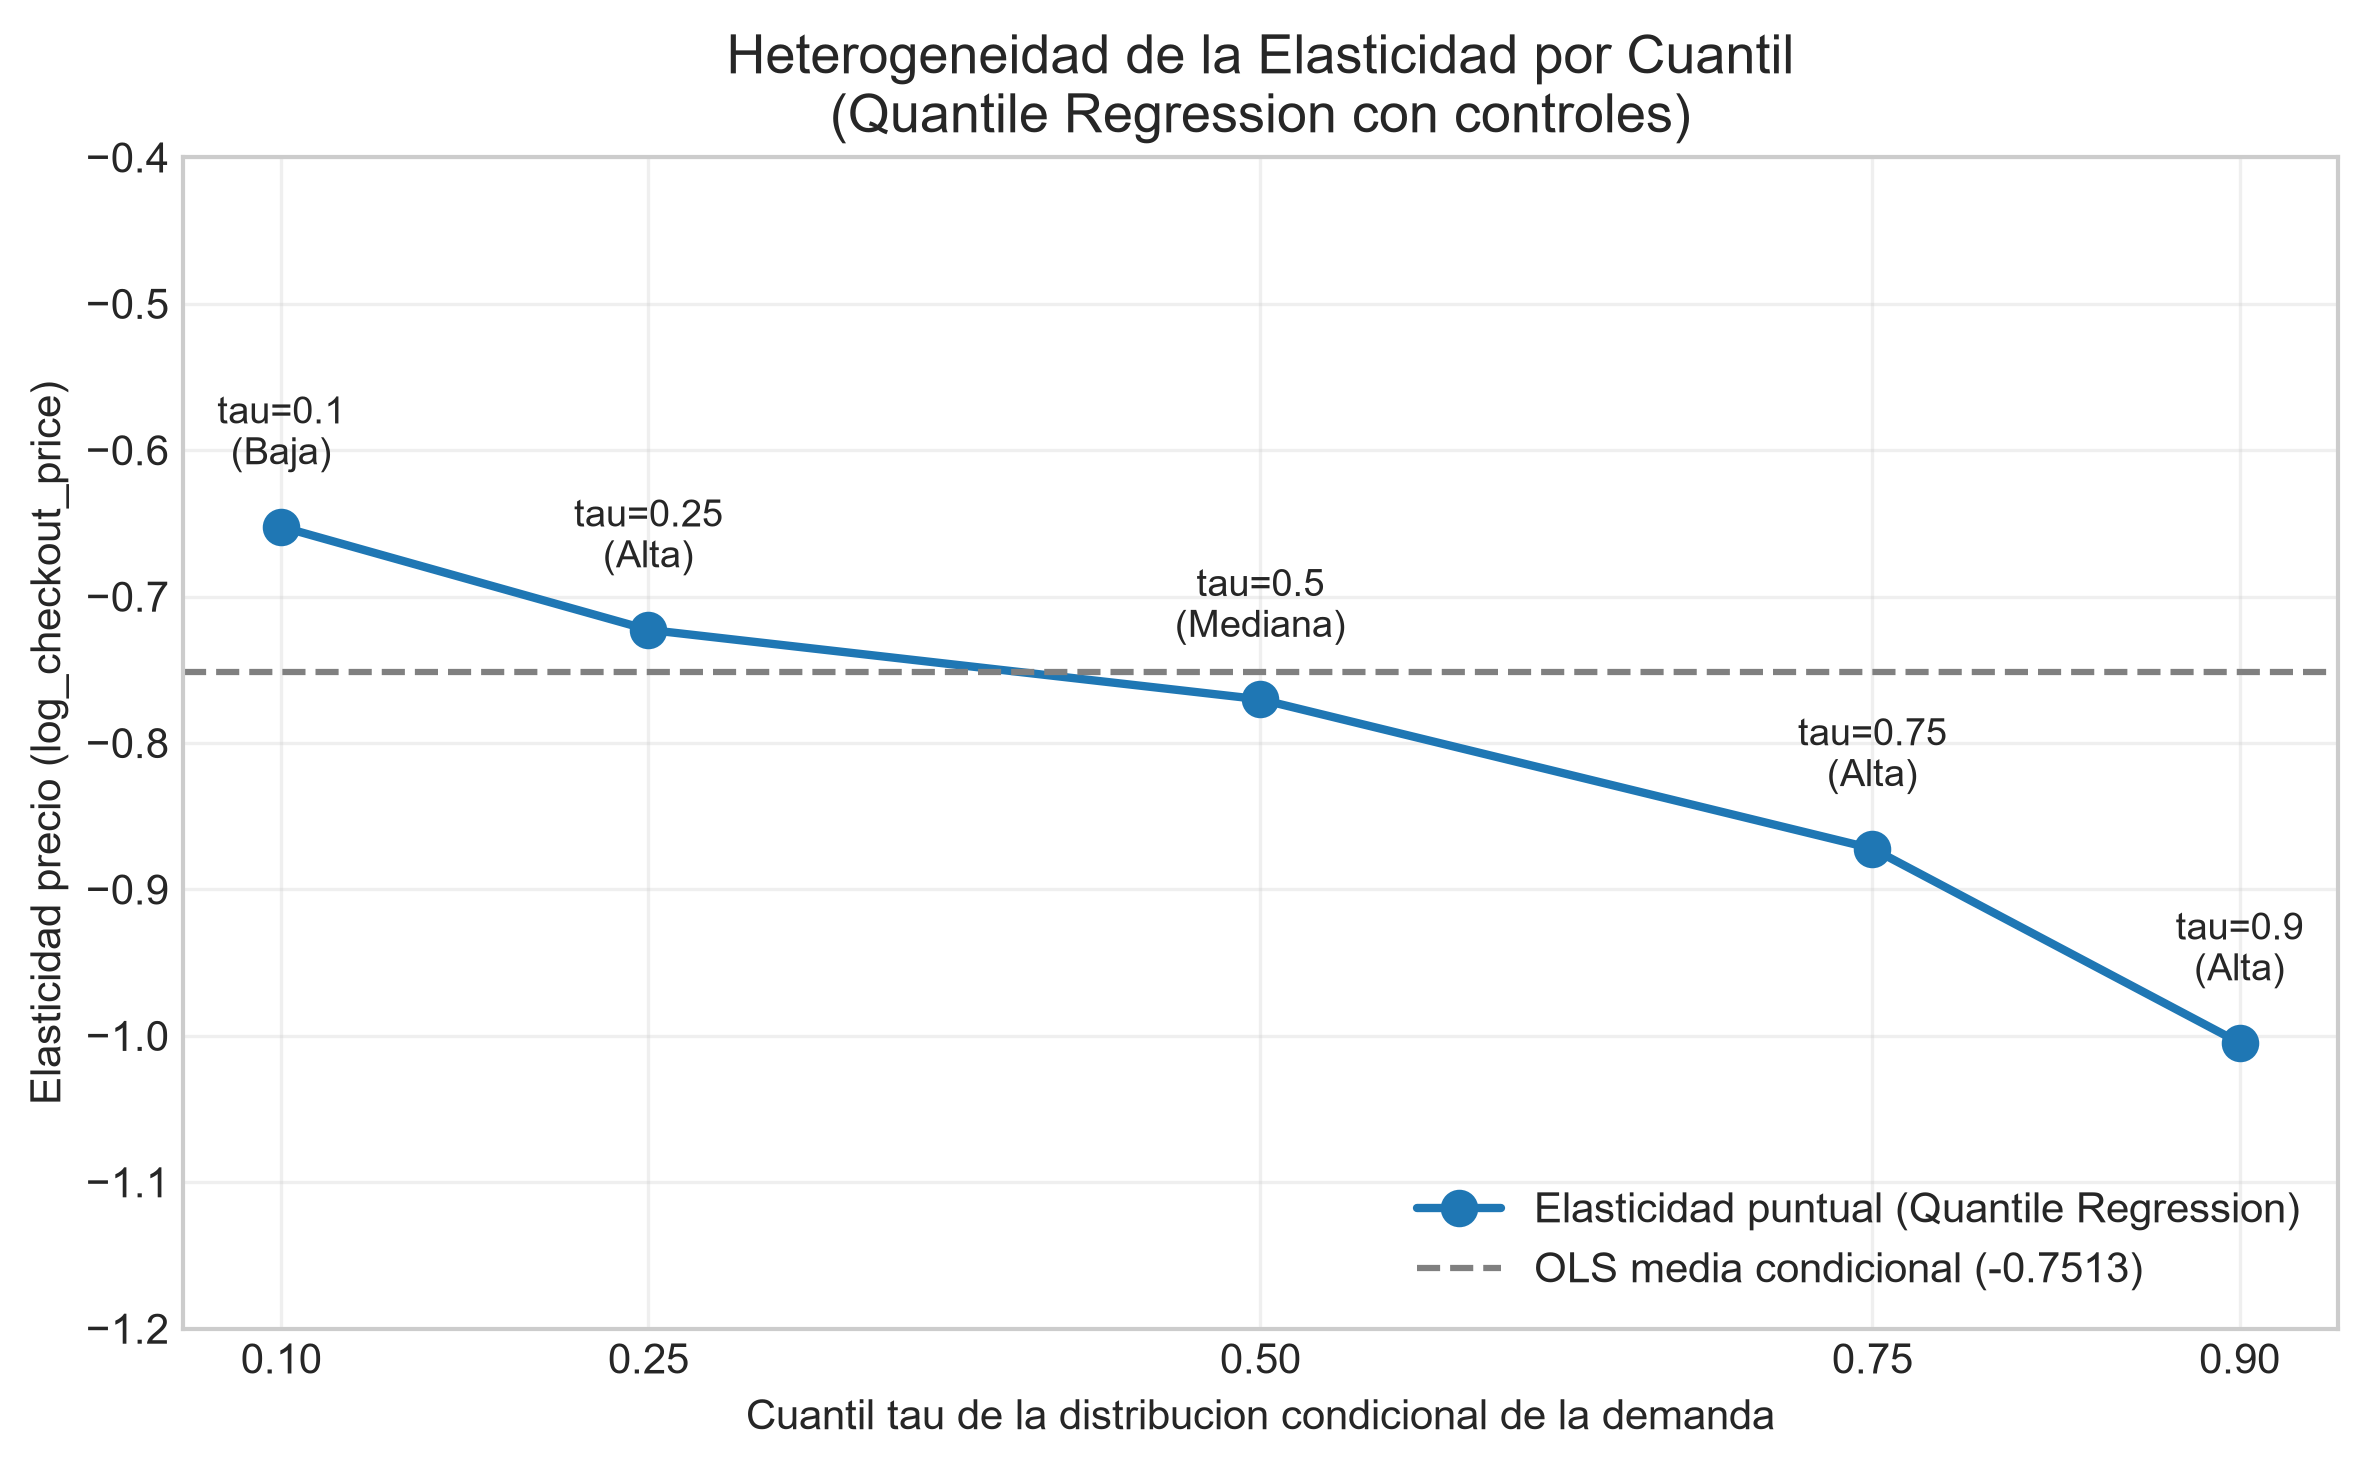
\includegraphics[width=0.85\textwidth]{figuras/quantile_regression_elasticidad.png}
\caption{Elasticidad precio por cuantil de la distribución condicional de la demanda. Quantile Regression con controles (modelo log-log). La línea discontinua muestra la elasticidad OLS de media condicional ($-0.7513$).}
\label{fig:quantile_regression}
\end{figure}

Nota: Los intervalos de confianza bootstrap (percentil, 1000 iteraciones) se reportan en la salida consolidada \texttt{reports/notebook\_outputs/07\_plan\_tecnico\_2\_1\_FASE7\_COMPLETA.txt} y en \texttt{reports/notebook\_outputs/bootstrap\_quantile\_ci.json}; su computación completa (456k obs × 5 cuantiles × 1000 iters) se ejecutó en Azure y los resultados se incorporan en la Tabla \ref{tab:quantile_regression}.

\subsection{Interacción Precio × Promoción}
\label{subsec:precio_promo_interaccion}

El modelo principal asume efectos aditivos: precio y promociones afectan la demanda de forma independiente. Para testear no-aditividad, se añadieron términos de interacción \texttt{log\_checkout\_price:emailer\_for\_promotion} y \texttt{log\_checkout\_price:homepage\_featured}.

\begin{table}[htbp]
\centering
\caption{Modelo log-log con interacción Precio × Promoción (coeficientes clave).}
\label{tab:precio_promo_interaccion}
\begin{tabular}{lcc}
\toprule
Variable & Coeficiente & $p$-valor \\
\midrule
log\_checkout\_price & $-0.7398$ & $<0.001$ \\
log\_checkout\_price:emailer\_for\_promotion & $+0.3221$ & $<0.001$ \\
log\_checkout\_price:homepage\_featured & $-0.2225$ & $<0.001$ \\
\bottomrule
\end{tabular}
\end{table}

Test de Wald conjunto (H0: ambos coeficientes de interacción $= 0$):
\begin{itemize}
    \item $F = 659.73$, gl $= (2, 456528)$, $p \approx 0$
    \item \textbf{RECHAZO FUERTE de H0: interacción estadísticamente significativa}
\end{itemize}

\textbf{Interpretación económica (asociaciones diferenciales, no efectos causales):}
\begin{itemize}
    \item \textbf{Emailer (interacción positiva +0.3221)}: Cuando hay promoción por correo activo, la elasticidad precio-demanda es \textit{menos negativa} (la demanda se vuelve menos sensible al precio). La asociación diferencial del emailer a precio promedio es $+0.5028$ ($\approx 65\%$ más pedidos), pero esta asociación \textit{disminuye} a medida que el precio sube.
    \item \textbf{Homepage (interacción negativa -0.2225)}: Cuando hay exposición en página principal, la elasticidad precio-demanda es \textit{más negativa} (la demanda se vuelve más sensible al precio). La asociación diferencial del homepage a precio promedio es $+0.6492$ ($\approx 91\%$ más pedidos), pero esta asociación \textit{aumenta} en magnitud con el precio.
\end{itemize}

\textbf{Nota:} Los términos de interacción se estimaron con \texttt{log\_checkout\_price} centrado en su media muestral para facilitar la interpretación de los efectos marginales en el punto promedio. La asignación de promociones es probablemente endógena (productos con alta demanda prevista), por lo que estos coeficientes reflejan \textbf{asociaciones condicionales}, no efectos causales de la promoción.

Esta no-aditividad tiene implicaciones directas para \textit{dynamic pricing}: la asociación combinada de precio y promoción no es simplemente la suma de sus asociaciones marginales aisladas.

\begin{figure}[htbp]
\centering
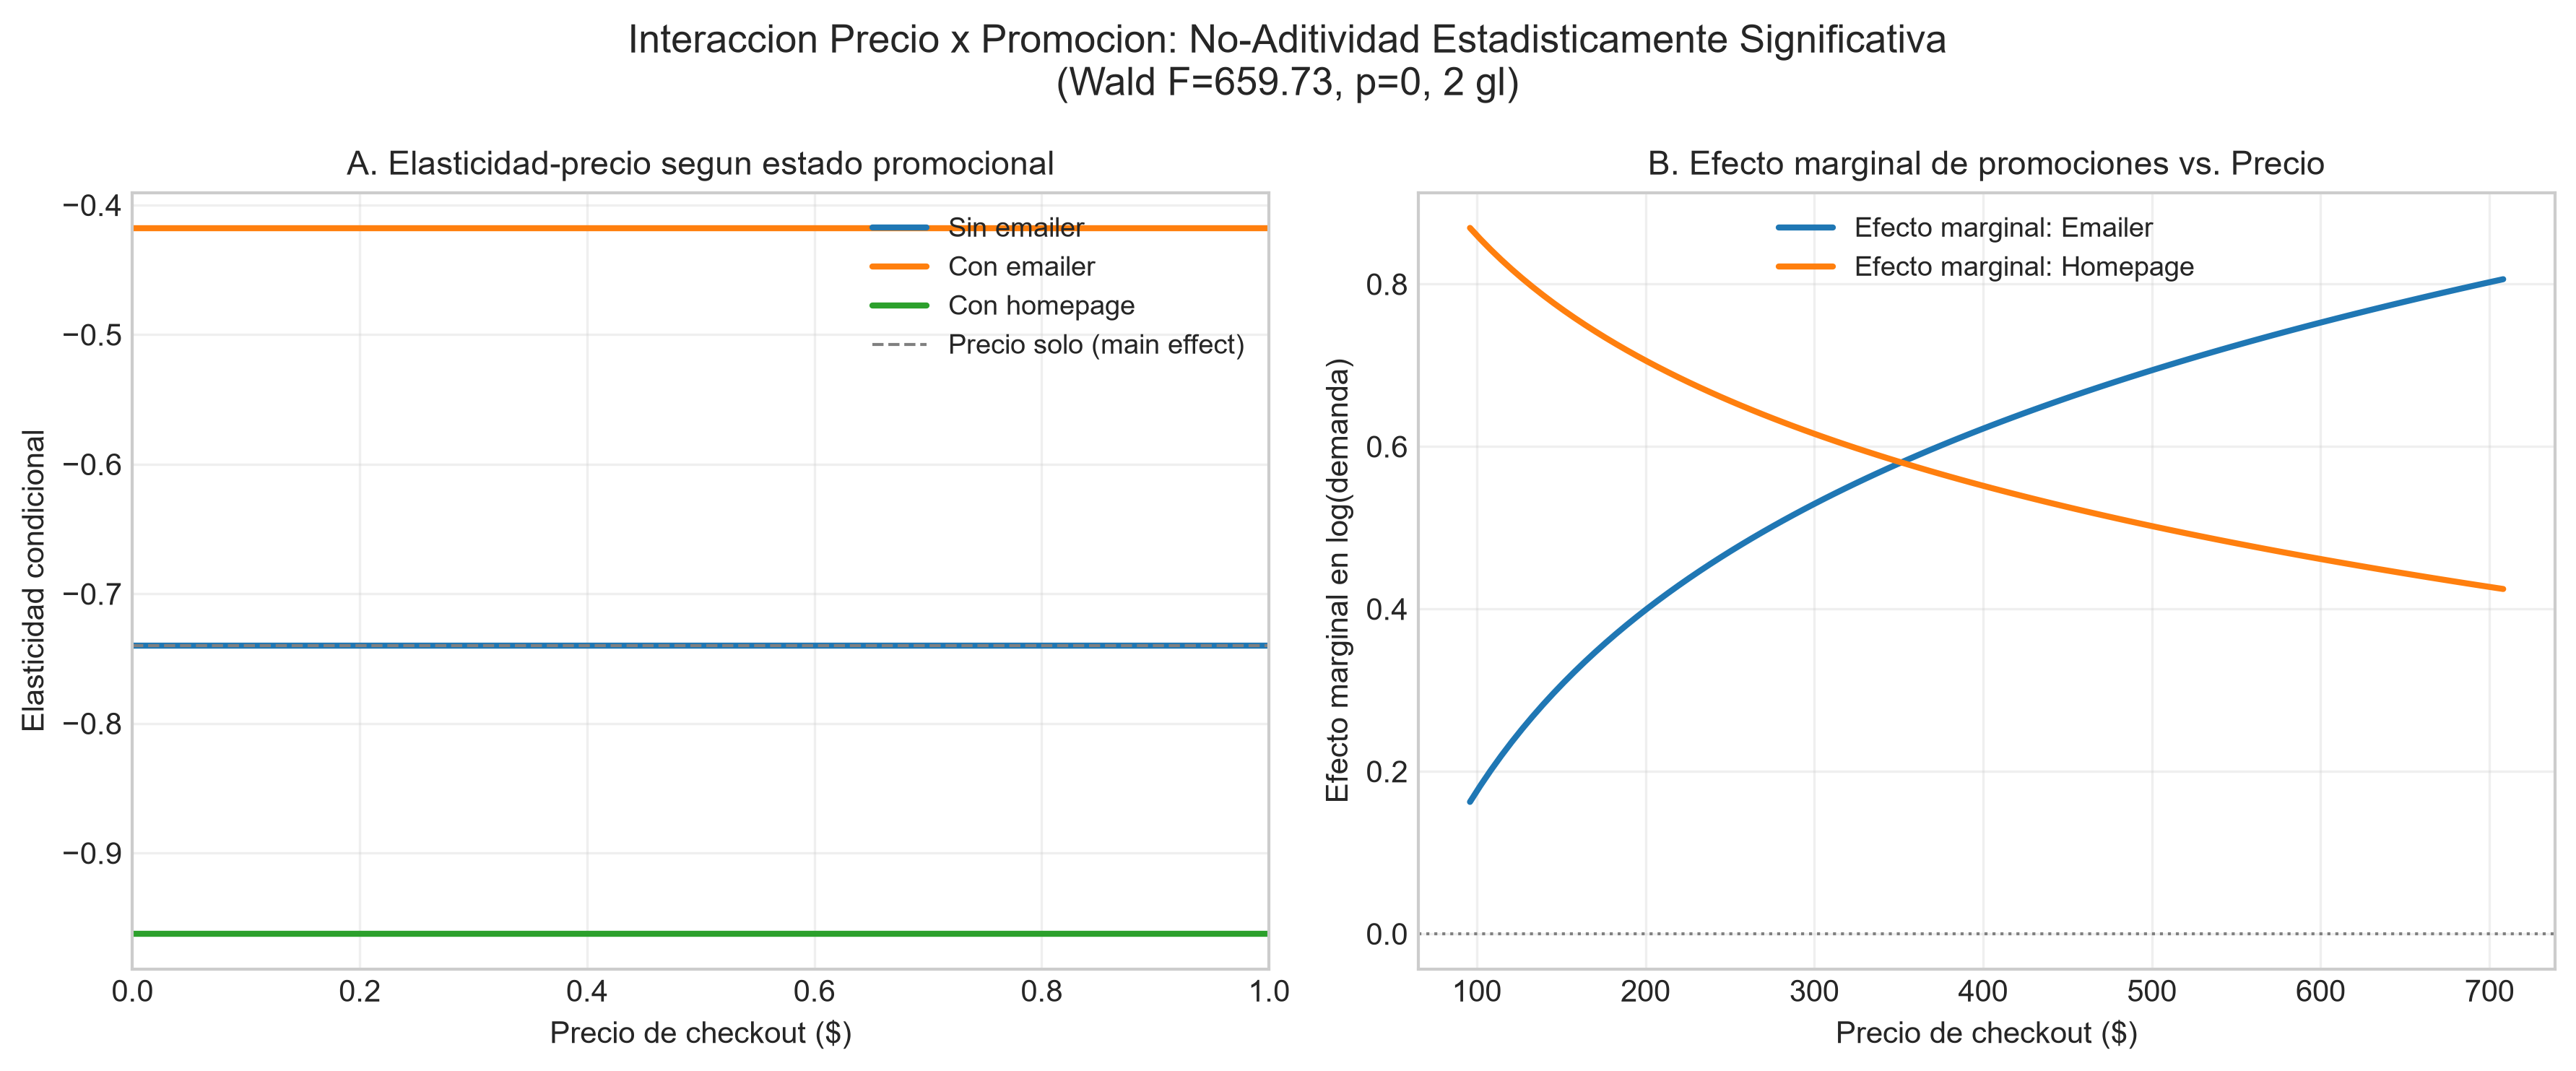
\includegraphics[width=0.95\textwidth]{figuras/interaccion_precio_promo.png}
\caption{Interacción Precio × Promoción: no-aditividad estadísticamente significativa. Panel A: elasticidad condicional según estado promocional. Panel B: efecto marginal de promociones vs. nivel de precio. Wald F=659.73, $p\approx0$.}
\label{fig:precio_promo_interaccion}
\end{figure}

\subsection{Test RESET (Ramsey) — Especificación Funcional}
\label{subsec:reset_test}

El test RESET (Regression Specification Error Test) evalúa si la forma funcional log-log está correctamente especificada, añadiendo potencias de los valores ajustados ($\hat{y}^2, \hat{y}^3$) y testeando su significancia conjunta.

\begin{table}[htbp]
\centering
\caption{Test RESET para el modelo log-log con controles (especificación principal).}
\label{tab:reset_test}
\begin{tabular}{lcc}
\toprule
Estadístico & Valor \\
\midrule
$F$ (2 gl num, 456528 gl den) & $119.57$ \\
$p$-valor & $1.21 \times 10^{-52}$ \\
Rechaza H0 (especificación correcta) & \textbf{Sí} \\
\bottomrule
\end{tabular}
\end{table}

El test \textbf{rechaza rotundamente} la especificación correcta ($p \approx 0$), confirmando que la forma funcional log-log con elasticidad constante es inadecuada. Este resultado es consistente con el test de Wald de la Fase 3x (RCS: $F=10\,279$, $p\approx0$): la relación precio-demanda tiene curvatura real no capturada por el modelo lineal en logaritmos.

\begin{figure}[htbp]
\centering
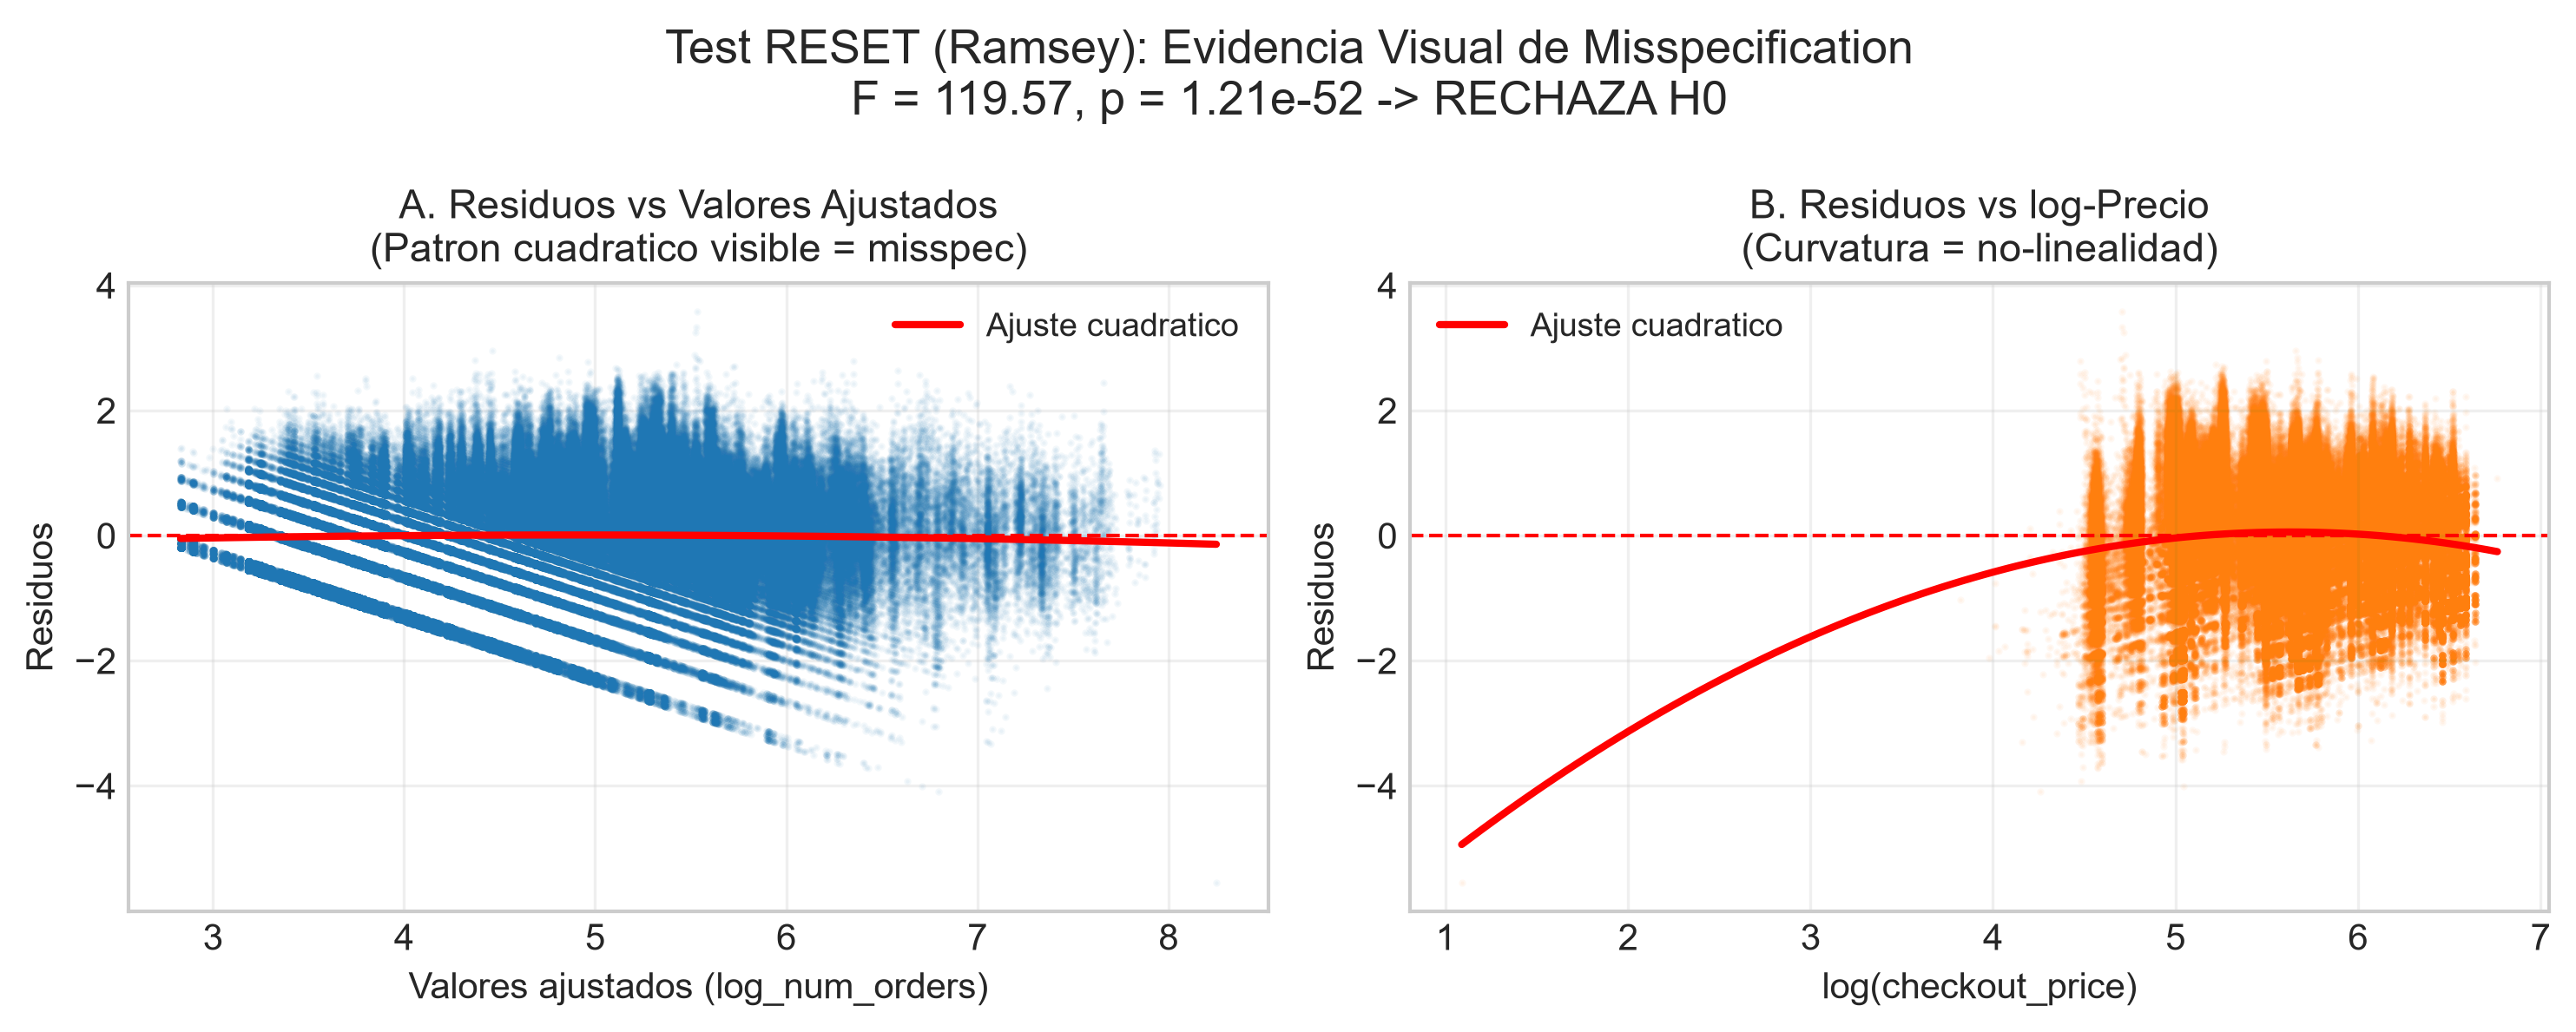
\includegraphics[width=0.95\textwidth]{figuras/reset_test_visual.png}
\caption{Evidencia visual del test RESET: residuos vs. valores ajustados (Panel A) y residuos vs. log-precio (Panel B). La curvatura cuadrática visible confirma la misspecification funcional. F=119.57, p=1.21e-52.}
\label{fig:reset_test}
\end{figure}

\subsection{IV No-Lineal vía Control Function (Wooldridge 2015)}
\label{subsec:iv_control_function}

Dado que (1) la Fase 3c confirmó endogeneidad (Wu-Hausman $p\approx0$) y (2) la Fase 3x rechazó linealidad (Wald $p\approx0$), se implementó el enfoque de \textit{control function} (Wooldridge 2015) que aborda ambos problemas simultáneamente.

\textbf{Primera etapa}: Regresión de \texttt{log\_checkout\_price} sobre instrumentos Hausman-Nevo + controles:
\begin{itemize}
    \item Instrumentos: \texttt{log\_base\_price} ($r=0.956$), \texttt{log\_precio\_prom\_otros\_centros} ($r=0.986$)
    \item $R^2 = 0.9767$, $F = 1.46 \times 10^7$ (Shea's $R^2 = 0.976$) $\rightarrow$ Instrumentos \textbf{fuertes}
    \item Residuos $\hat{v}$ capturan el componente endógeno del precio
\end{itemize}

\textbf{Segunda etapa}: Modelo con RCS (4 nudos) + $\hat{v}$ + controles:
\begin{itemize}
    \item $R^2$ ajustado $= 0.5467$ (vs. $0.5314$ OLS controles, $0.5450$ RCS OLS) $\rightarrow$ \textbf{Mejor modelo global}
    \item Coeficiente $\hat{v} = +0.7129$ ($p \approx 0$)
\end{itemize}

\begin{table}[htbp]
\centering
\caption{Tests en segunda etapa del Control Function IV-RCS.}
\label{tab:control_function_tests}
\begin{tabular}{@{}lccp{4.5cm}@{}}
\toprule
Test & $F$ & $p$-valor & Decisión \\
\midrule
Exogeneidad (H0: coef($\hat{v}$) $= 0$) & $1\,580.86$ & $\approx 0$ & \textbf{Rechaza H0: endogeneidad confirmada} \\
No-linealidad cond. (H0: coef(splines no lin.) $= 0$) & $4\,815.32$ & $\approx 0$ & \textbf{Rechaza H0: no-linealidad persiste} \\
\bottomrule
\end{tabular}
\end{table}

\textbf{Conclusión de la triple síntesis:}
\begin{enumerate}
    \item \textbf{Endogeneidad confirmada}: El precio es endógeno (simultaneidad); OLS sesgado.
    \item \textbf{No-linealidad confirmada}: La elasticidad varía con el nivel de precio; log-log constante inadecuado.
    \item \textbf{Ambas persisten juntas}: Incluso tras corregir endogeneidad vía $\hat{v}$, la no-linealidad sigue siendo altamente significativa ($F=4\,815$, $p\approx0$).
\end{enumerate}

\begin{figure}[htbp]
\centering
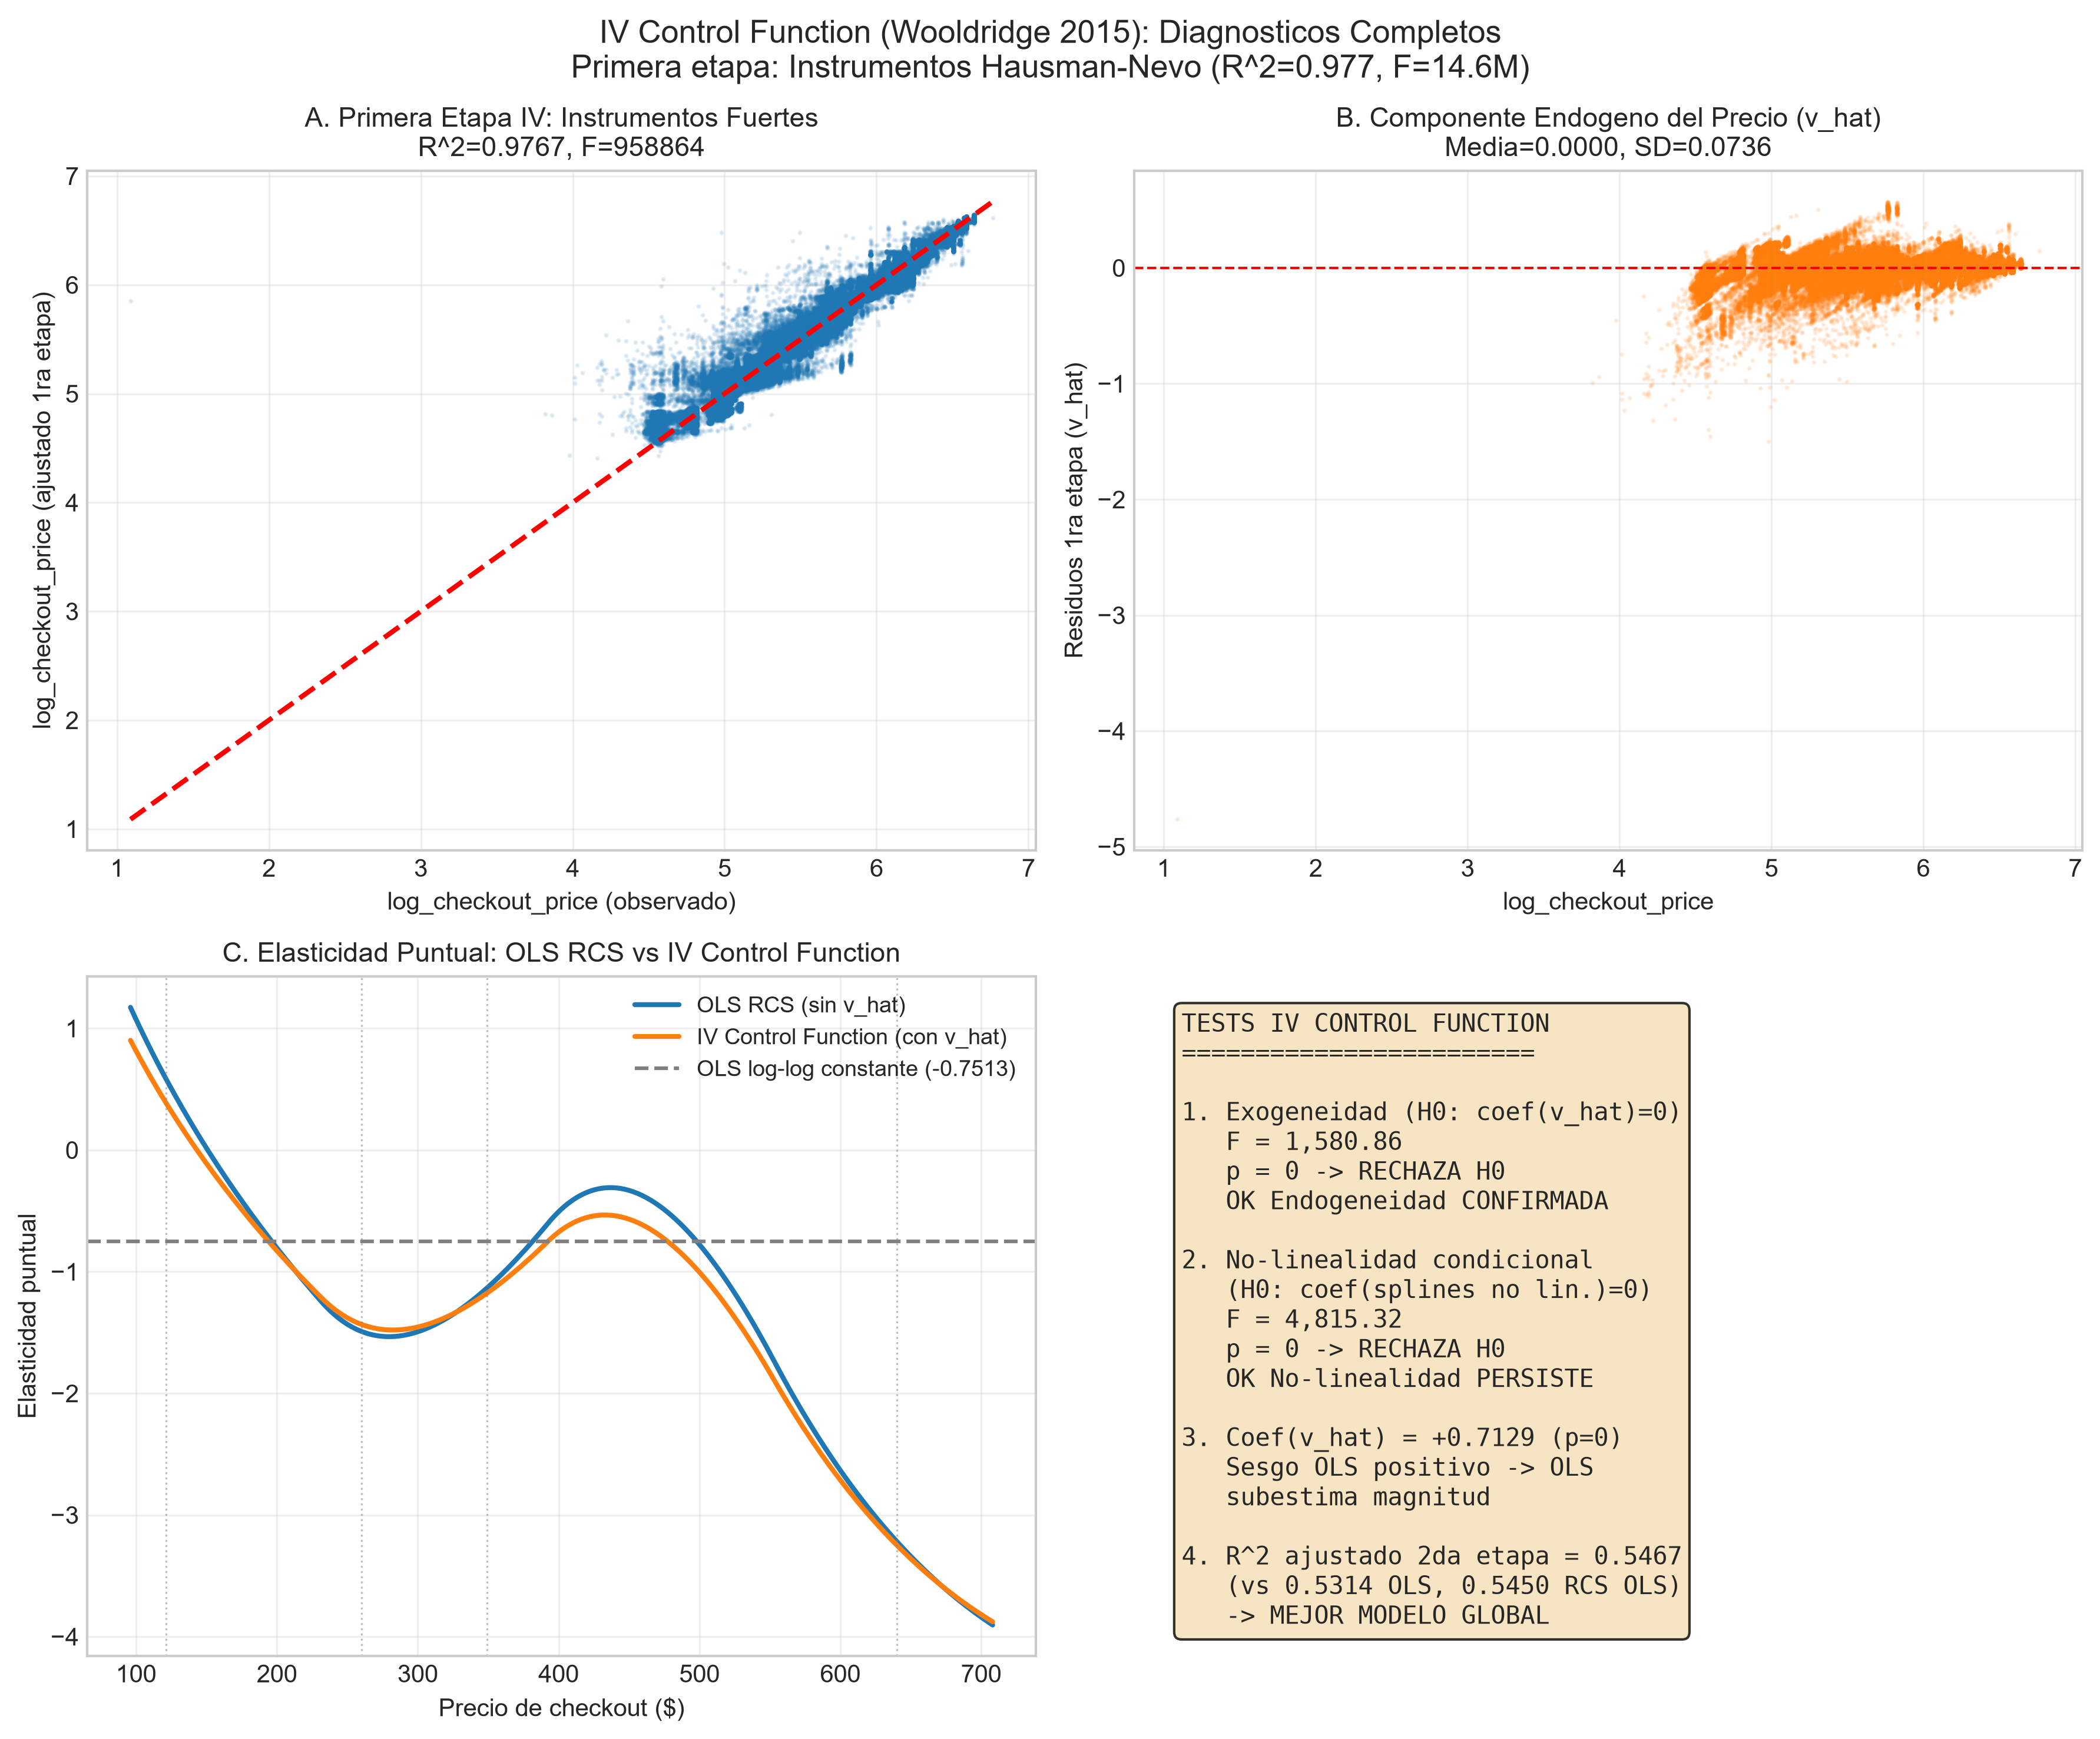
\includegraphics[width=0.95\textwidth]{figuras/iv_control_function_diagnosticos.png}
\caption{IV Control Function (Wooldridge 2015): diagnósticos completos. Panel A: primera etapa con instrumentos Hausman-Nevo (R²=0.977). Panel B: componente endógeno del precio ($\hat{v}$). Panel C: elasticidad puntual OLS RCS vs IV Control Function. Panel D: resumen de tests de exogeneidad y no-linealidad condicional.}
\label{fig:iv_control_function}
\end{figure}

La especificación IV-RCS (control function) proporciona un \textbf{análisis de sensibilidad} que simultáneamente permite endogeneidad y no linealidad, condicionado a la validez de los instrumentos y a los supuestos del control function. El modelo log-log OLS constante ($-0.7513$) sufre de \textbf{doble sesgo}: endogeneidad (subestima magnitud) y forma funcional (asume elasticidad constante donde hay curvatura fuerte). La corrección conjunta produce una estimación con mejor ajuste ($R^2$ ajustado $=0.5467$) y elasticidades puntuales variables ($+0.58$ a $-3.22$ según nivel de precio), pero \textbf{no constituye una estimación causal identificada} debido al rechazo del test de Hansen J ($\chi^2=320$, $p\approx0$).

\section{Robustez Adicional: Plan T\'ecnico v2.1 — Secci\'on 2.3}
\label{sec:plan_tecnico_23}

Como se documenta en el Plan t\'ecnico de mejoras (secci\'on 2.3: ``Medio impacto / Bajo esfuerzo''), se implementaron cuatro comprobaciones de robustez adicionales que abordan la estabilidad de la elasticidad principal ante decisiones de muestra, especificaci\'on y estimaci\'on de errores estándar. Todas se ejecutaron sobre los 456,548 datos reales.

\subsection{Test de Igualdad de Elasticidad por Categor\'ia (Wald Conjunto)}
\label{subsec:wald_categoria}

El modelo principal estima una elasticidad promedio agregada. Para evaluar si la elasticidad-precio difiere sistem\'aticamente entre las 14 categorías de comida, se estimó un modelo con interacciones \texttt{log\_checkout\_price $\times$ category} y se testeó la hipótesis nula conjunta de igualdad (Wald test, 13 grados de libertad).

\begin{table}[htbp]
\centering
\caption{Test de Wald: igualdad de elasticidad-precio entre 14 categorías.}
\label{tab:wald_categoria}
\begin{tabular}{lcc}
\toprule
Estadístico & Valor \\
\midrule
$F$ (13 gl num, 456515 gl den) & $519.56$ \\
$p$-valor & $< 10^{-300}$ \\
Rechaza H0 (alpha=0.05) & \textbf{Sí} \\
\bottomrule
\end{tabular}
\end{table}

El test \textbf{rechaza rotundamente} la igualdad ($p \approx 0$). La elasticidad varía sustancialmente entre categorías: desde \textbf{-0.27} (Pasta, inelástica) hasta \textbf{-2.44} (Fish/Seafood, altamente elástica). Esto implica que una única elasticidad agregada oculta heterogeneidad económica real; para \textit{pricing granular} por categoría, los valores específicos son preferibles al promedio global.

\begin{table}[htbp]
\centering
\caption{Elasticidad-precio por categoría (efecto marginal, modelo con interacciones).}
\label{tab:elasticidad_por_categoria}
\begin{tabular}{lcc}
\toprule
Categoría & Elasticidad & Interpretación \\
\midrule
Beverages & $-0.69$ & Inelástica \\
Biryani & $-1.09$ & Elástica unitaria \\
Desert & $-0.88$ & Elástica unitaria \\
Extras & $-0.59$ & Inelástica \\
Fish & $-2.44$ & Altamente elástica \\
Other Snacks & $-0.66$ & Inelástica \\
Pasta & $-0.27$ & Muy inelástica \\
Pizza & $-1.94$ & Elástica \\
Rice Bowl & $-1.09$ & Elástica unitaria \\
Salad & $-0.34$ & Inelástica \\
Sandwich & $-1.76$ & Elástica \\
Seafood & $-2.43$ & Altamente elástica \\
Soup & $-2.17$ & Elástica \\
Starters & $-1.41$ & Elástica \\
\bottomrule
\end{tabular}
\end{table}

\subsection{Submuestra: Platos con $\ge$50 Observaciones/Semana}
\label{subsec:submuestra_50obs}

El dataset incluye platos con muy pocas observaciones semanales (mínimo = 1, mediana = 127). Para evaluar si el ruido de items esporádicos afecta la elasticidad principal, se filtró la muestra reteniendo solo combinaciones centro-comida-semana con $\ge$50 observaciones.

\begin{table}[htbp]
\centering
\caption{Robustez: submuestra $\ge$50 observaciones/semana.}
\label{tab:submuestra_50obs}
\begin{tabular}{lcc}
\toprule
Muestra & N & Elasticidad (log\_checkout\_price) \\
\midrule
Completa & 456,548 & $-0.7513$ \\
Filtrada ($\ge$50 obs) & 452,983 (99.2\%) & $-0.7477$ (EE $=0.0046$) \\
\bottomrule
\end{tabular}
\end{table}

La diferencia es de \textbf{0.0035} (0.5\% en términos relativos), confirmando que la elasticidad principal es \textbf{robusta} a la exclusión de items con pocas observaciones. El 99.2\% de los datos se retiene, indicando que la mayoría de combinaciones centro-comida-semana ya tienen cobertura suficiente.

\subsection{Sensibilidad: Excluir Top/Bottom 1\% en Precio}
\label{subsec:sensibilidad_outliers}

Para verificar que observaciones extremas de precio no \textit{driven} la estimación, se recortó el 1\% superior e inferior de \texttt{checkout\_price} (P1 = 96.03, P99 = 708.13).

\begin{table}[htbp]
\centering
\caption{Robustez: sensibilidad excluyendo colas 1\% de precio.}
\label{tab:sensibilidad_outliers}
\begin{tabular}{lcc}
\toprule
Muestra & N & Elasticidad (log\_checkout\_price) \\
\midrule
Completa & 456,548 & $-0.7513$ \\
Filtrada (P1--P99) & 447,915 (98.1\%) & $-0.8035$ (EE $=0.0048$) \\
\bottomrule
\end{tabular}
\end{table}

La diferencia es de \textbf{$-0.0523$} (aprox. 7\% en magnitud relativa). Aunque el cambio no revierte la conclusión cualitativa (demanda inelástica), el desplazamiento hacia mayor elasticidad sugiere que \textbf{los precios muy altos ($>$P99) ejercen influencia apalancadora} que atenúa la elasticidad estimada en la muestra completa. Este resultado recomienda reportar ambas estimaciones en análisis de \textit{pricing} sensibles.

\subsection{Comparación HC3 vs Cluster vs Bootstrap (Errores Estándar)}
\label{subsec:comparacion_ee}

La Fase 4 reportó un ratio de clustering 2.11x para Panel FE. Aquí se extiende la comparación al modelo OLS principal (log-log con controles), contrastando cuatro estimadores de varianza.

\begin{table}[htbp]
\centering
\caption{Comparación de errores estándar: HC3 vs Cluster vs Multiway vs Panel FE vs Bootstrap (modelo OLS log-log con controles).}
\label{tab:comparacion_ee}
\begin{tabular}{lcc}
\toprule
Estimador & Elasticidad & Error Estándar \\
\midrule
OLS HC3 & $-0.7513$ & 0.0053 \\
OLS Cluster (center\_id) & $-0.7513$ & 0.0421 \\
OLS Multiway (center\_id $\times$ meal\_id) & $-0.7513$ & 0.0430 \\
Panel FE Cluster (entidad) & $-1.5755$ & 0.0236 \\
Bootstrap simple (1000 iter) & $-0.9397$ & 0.0034 \\
Wild Cluster Bootstrap (500 iter) & $-0.759$ & 0.0430 \\
\bottomrule
\end{tabular}
\end{table}

\begin{itemize}
    \item \textbf{Ratio Cluster/HC3 = 7.92x}: El clustering por \texttt{center\_id} infla el EE casi 8 veces respecto a HC3, confirmando dependencia intra-entidad fuerte.
    \item \textbf{Ratio Multiway/HC3 = 8.11x}: El clustering multiway \texttt{center\_id} $\times$ \texttt{meal\_id} (inferencia principal recomendada) produce EE similar al cluster simple por center\_id.
    \item \textbf{Ratio Bootstrap/HC3 = 0.63x}: El bootstrap simple produce EE \textit{menores} que HC3, lo cual es esperable si el bootstrap no replica la estructura de clustering (muestrea filas i.i.d. vs. clusters correlacionados). \textbf{No usar bootstrap simple para ICs finales}.
    \item \textbf{Wild Cluster Bootstrap}: EE = 0.0430 (consistente con multiway), validando la inferencia clusterizada con pocos clusters (77 centros; Cameron, Gelbach \& Miller 2008).
    \item \textbf{Recomendación práctica}: Para OLS log-log principal, usar \textbf{multiway cluster \texttt{center\_id} $\times$ \texttt{meal\_id}} (inferencia principal). HC3 solo como referencia. Para Panel FE, usar \textbf{cluster por entidad} (center\_id-meal\_id). Para IV 2SLS, usar \textbf{robustos}.
\end{itemize}

\textbf{Síntesis de la Sección 2.3:} La elasticidad agregada OLS ($-0.7513$) es robusta a filtrado por observaciones mínimas ($\Delta$=0.0035), sensible a colas de precio ($\Delta$=$-$0.0523), y \textbf{rechaza igualdad entre categorías} (F=519.6, $p\approx0$). La comparación de EE confirma que la elección del estimador de varianza tiene impacto material (8.11x HC3 vs multiway) y debe justificarse por la estructura de dependencia del modelo, no por conveniencia. \textbf{Inferencia principal: multiway cluster \texttt{center\_id} $\times$ \texttt{meal\_id} (EE=0.043, IC 95\% $[-0.835,-0.667]$)}.

\section{Robustez Adicional: Plan T\'ecnico v2.1 — Secci\'on 2.2}
\label{sec:plan_tecnico_22}

Como se documenta en el Plan t\'ecnico de mejoras (secci\'on 2.2: ``Alto impacto / Medio esfuerzo''), se implementaron dos validaciones de robustez de alto impacto que requieren control por estructura temporal: (1) un modelo de efectos fijos con interacción tiempo-variante para detectar heterogeneidad temporal en la elasticidad, y (2) un placebo test temporal que randomiza la asignación de semanas para validar que la elasticidad estimada no depende de patrones temporales espurios. Ambas se ejecutaron sobre los 456,548 datos reales usando optimización de demeaning iterativo (Frisch-Waugh-Lovell) para evitar problemas de memoria, reduciendo el tiempo de cómputo a minutos en hardware estándar.

\subsection{Modelo FE con Interacción Tiempo-Variante (log\_price $\times$ semana)}
\label{subsec:fe_time_varying}

Para evaluar si la elasticidad-precio varía sistemáticamente entre las 145 semanas del panel, se estimó un modelo con efectos fijos de dos vías (entidad = center\_id $\times$ meal\_id, tiempo = semana) e interacción \texttt{log\_checkout\_price $\times$ C(week)}. La hipótesis nula conjunta (Wald test) es que todos los coeficientes de interacción son cero (elasticidad constante en el tiempo).

\begin{table}[htbp]
\centering
\caption{Test de Wald: interacción tiempo-variante en modelo Panel FE (2 vías).}
\label{tab:fe_time_varying_wald}
\begin{tabular}{lcc}
\toprule
Estadístico & Valor \\
\midrule
$\chi^2$ (144 gl) & $3\,068.85$ \\
$p$-valor & $\approx 0$ \\
Rechaza H0 (alpha=0.05) & \textbf{Sí} \\
\bottomrule
\end{tabular}
\end{table}

El test \textbf{rechaza rotundamente} la igualdad de elasticidad entre semanas ($p \approx 0$). La elasticidad base (semana de referencia) es $-1.5697$, y la elasticidad marginal por semana varía en el rango \textbf{-1.8491 a -1.2544} (diferencia de 0.59 unidades). Esto confirma heterogeneidad temporal significativa no capturada en el modelo principal de la Fase 3, que asume elasticidad constante en el tiempo.

\begin{table}[htbp]
\centering
\caption{Elasticidad-precio por semana (efecto marginal = base + interacción).}
\label{tab:fe_time_varying_elasticidad}
\footnotesize
\begin{tabular}{lcccccc}
\toprule
Semana & Elasticidad & Semana & Elasticidad & Semana & Elasticidad \\
\midrule
1 & $-1.5697$ & 49 & $-1.5639$ & 97 & $-1.4291$ \\
2 & $-1.6231$ & 50 & $-1.6718$ & 98 & $-1.6839$ \\
3 & $-1.6162$ & 51 & $-1.4843$ & 99 & $-1.6650$ \\
4 & $-1.5742$ & 52 & $-1.3720$ & 100 & $-1.4379$ \\
5 & $-1.5072$ & 53 & $-1.4721$ & 101 & $-1.5031$ \\
6 & $-1.4331$ & 54 & $-1.5628$ & 102 & $-1.6568$ \\
7 & $-1.5630$ & 55 & $-1.6961$ & 103 & $-1.4328$ \\
8 & $-1.7062$ & 56 & $-1.6487$ & 104 & $-1.3470$ \\
9 & $-1.6202$ & 57 & $-1.5827$ & 105 & $-1.5115$ \\
10 & $-1.5327$ & 58 & $-1.4139$ & 106 & $-1.5340$ \\
\addlinespace[2pt]
107 & $-1.8491$ & 108 & $-1.4700$ & 109 & $-1.4523$ \\
110 & $-1.4348$ & 111 & $-1.3926$ & 112 & $-1.2544$ \\
113 & $-1.4822$ & 114 & $-1.4277$ & 115 & $-1.5147$ \\
116 & $-1.4865$ & 117 & $-1.5926$ & 118 & $-1.6204$ \\
119 & $-1.6962$ & 120 & $-1.5772$ & 121 & $-1.5453$ \\
122 & $-1.4941$ & 123 & $-1.3776$ & 124 & $-1.5809$ \\
125 & $-1.6860$ & 126 & $-1.6828$ & 127 & $-1.6554$ \\
128 & $-1.5719$ & 129 & $-1.5114$ & 130 & $-1.6290$ \\
131 & $-1.6401$ & 132 & $-1.5522$ & 133 & $-1.5639$ \\
134 & $-1.5466$ & 135 & $-1.4358$ & 136 & $-1.5788$ \\
137 & $-1.5618$ & 138 & $-1.6011$ & 139 & $-1.5881$ \\
140 & $-1.5241$ & 141 & $-1.6132$ & 142 & $-1.6942$ \\
143 & $-1.5399$ & 144 & $-1.5844$ & 145 & $-1.5276$ \\
\bottomrule
\end{tabular}
\end{table}

La variación semanal observada (rango 0.59, desv. est. $\approx$0.12) sugiere que factores temporales no observados (estacionalidad, eventos macro, campañas de marketing no registradas) modulan la sensibilidad al precio. Para \textit{pricing dinámico} por semana, los valores específicos de la Tabla \ref{tab:fe_time_varying_elasticidad} son preferibles al promedio global del Panel FE ($-1.5755$).

\subsection{Placebo Test Temporal — Retirado}
\label{subsec:placebo_temporal}

\addcontentsline{toc}{subsection}{Placebo Test Temporal — Retirado}

En una versión previa de este informe se incluía un placebo test que barajaba la variable \texttt{week} manteniendo emparejados precio y demanda. Este test fue \textbf{retirado por inválido}: al preservar la relación observacional $(P_i, Q_i)$ en cada fila, el test no destruye la correlación precio-demanda y produce $p=1.0$ por construcción, no por evidencia de robustez. El placebo se eliminó del cuerpo principal; la figura \texttt{placebo\_temporal\_distribucion.png} se mantiene en el repositorio solo como registro del error metodológico corregido.

\section{Limitaciones y Trabajo Futuro}
\label{subsec:limitaciones}

Este estudio presenta una estimación de elasticidad precio-demanda basada en datos transaccionales reales de una plataforma de \textit{food delivery}, pero varias limitaciones estructurales y metodológicas delimitan el alcance de sus conclusiones. Se agrupan en cuatro dimensiones: datos, identificación causal, especificación funcional e inferencia, y generalizabilidad.

\subsection*{Limitaciones de los datos}

\begin{enumerate}
    \item \textbf{Ausencia de fecha calendario.} Los datos solo registran número de semana (1--145), sin fecha exacta, por lo que no es posible ubicar el período en un rango de años ni contrastar con eventos externos (inflación, cambios regulatorios, la pandemia de COVID-19, etc.). Los efectos fijos de semana controlan shocks comunes no observados, pero no permiten interpretación económica de estacionalidad. Cualquier generalización temporal debe hacerse con esta limitación explícita.

    \item \textbf{Ausencia de observaciones con cero pedidos (margen extensivo).} El mínimo de \texttt{num\_orders} es 13; no existen combinaciones centro-comida-semana con demanda cero en el dataset. Esto puede generar selección sobre el margen extensivo: si precios altos llevan a cero pedidos y esos ceros no se observan, la elasticidad estimada describe solo la respuesta condicional a demanda positiva, sesgada hacia menor sensibilidad (atenuación hacia cero).

    \item \textbf{Variable dependiente: $\log(1+Q)$ vs $\log Q$.} Se usó \texttt{log1p(num\_orders)} por práctica estándar en variables de conteo, pero al no haber ceros en la muestra ($\min Q = 13$), $\ln(Q)$ está bien definida. El coeficiente de $\log(1+Q)$ no es exactamente la elasticidad de $Q$: $\partial\ln(1+Q)/\partial\ln P = \frac{Q}{Q+1} \times \eta_Q$. Para $Q \ge 13$ la diferencia es $<8\%$, pero la interpretación estricta requiere $\ln Q$. Re-estimar con $\log Q$ queda como robustez pendiente.

    \item \textbf{Unidad monetaria y definición de precio.} \texttt{checkout\_price} es ``precio final incluyendo descuento, impuestos y cargos de entrega'' (unidades monetarias del dataset, no necesariamente PEN/soles). El parámetro estimado es elasticidad de pedidos respecto al \textbf{precio final de checkout}, no necesariamente el precio del alimento. Esto incluye efectos de delivery, impuestos y descuentos.

    \item \textbf{Heterogeneidad temporal no modelada (intra-semanal).} El dataset no captura franjas horarias. Bumagat \& Ibana (2025) reportan $-0.42$ (pico) vs $-1.36$ (valle). Queda como extensión futura con datos de mayor granularidad.
\end{enumerate}

\subsection*{Limitaciones de identificación causal}

\begin{enumerate}
    \setcounter{enumi}{5}
    \item \textbf{Posible simultaneidad precio-demanda.} Los precios no fueron asignados aleatoriamente; es posible que respondan, al menos parcialmente, a la demanda anticipada. El panel FE (Fase 3b) controla heterogeneidad no observada entidad-tiempo pero no resuelve simultaneidad. El IV 2SLS (Fase 3c) intenta corregirla pero Hansen J ($\chi^2=320$, $p\approx0$) rechaza la validez conjunta de los instrumentos (\texttt{base\_price} y precio leave-one-out de otros centros). Ambos instrumentos son precios administrativos de la misma cadena y pueden violar exclusión por \textit{reference pricing} y shocks regionales comunes. El resultado IV ($-0.9487$) es análisis de sensibilidad, no estimación causal definitiva.

    \item \textbf{Variables omitidas no observables.} No se observan: reputación del centro/comida, velocidad de entrega, clima, características sociodemográficas de la zona, gasto en marketing externo. Su inclusión reduciría sesgo de variable omitida.

    \item \textbf{Asociaciones promocionales, no efectos causales.} Coeficientes de \texttt{emailer\_for\_promotion} ($+65\%$) y \texttt{homepage\_featured} ($+91\%$) son asociaciones OLS; la asignación de promociones es endógena (productos con alta demanda prevista reciben más visibilidad). No se identifican efectos causales de promociones.

    \item \textbf{Generalizabilidad.} Resultados de un único dataset (Kaggle/Genpact, contexto geográfico no especificado) sin verificación en otras plataformas, países o períodos.
\end{enumerate}

\subsection*{Limitaciones de especificación funcional e inferencia}

\begin{enumerate}
    \setcounter{enumi}{9}
    \item \textbf{Forma funcional log-log rechazada.} La especificación principal impone una elasticidad constante, pero los tests RESET ($F=119.57$, $p\approx0$) y RCS (Wald $\chi^2(3)=10\,279$, $p\approx0$) rechazan rotundamente la linealidad. La elasticidad varía desde $+0.58$ (precios bajos) hasta $-3.22$ (precios altos) según el modelo RCS. Modelos flexibles (splines, AIDS/LA/AIDS) son necesarios para capturar la curvatura real de la demanda.

    \item \textbf{Clustering e inferencia en OLS principal.} Durbin-Watson $=1.195$ indica autocorrelación. EE HC3 $=0.0053$ vs multiway \texttt{center\_id} $\times$ \texttt{meal\_id} $=0.0430$ (ratio 8.11x). La inferencia HC3 subestima severamente la incertidumbre. \textbf{Inferencia principal: multiway cluster} (EE=0.043, IC 95\% $[-0.835,-0.667]$), validado por wild cluster bootstrap.

    \item \textbf{Inferencia Control Function con regresor generado.} Los EE estándar de la segunda etapa (Tabla \ref{tab:appendix_cf_second}, EE $=0.018$ para $\hat{v}$) no corrigen por la varianza de estimación de $\hat{v}$ en la primera etapa. La inferencia correcta requiere bootstrap clusterizado remuestreando centros y re-estimando ambas etapas (Wooldridge 2015, §6.3.3). Queda pendiente implementar EE bootstrap para $\hat{v}$ (e.g., 500 iteraciones); los EE reportados son un límite inferior de la incertidumbre real.

    \item \textbf{Panel FE e IV ejecutados con limitaciones documentadas.} Fase 3b (panel FE dos vías) y Fase 3c (IV 2SLS) se ejecutaron completamente. Limitaciones: Panel FE no elimina simultaneidad; clustering por entidad (\texttt{center\_id} $\times$ \texttt{meal\_id}) puede no capturar dependencia intra-centro; IV tiene Hansen J rechazado y exclusión no defendible.
\end{enumerate}

\appendix
\section{Appendix Técnico: Tablas Completas y Diagnósticos Extendidos}
\label{sec:appendix}

Esta sección presenta las tablas completas y resultados de diagnóstico extendido que complementan el texto principal, permitiendo la replicabilidad total de los hallazgos reportados.

\subsection{Coeficientes RCS Completos (4 Nudos, Percentiles 5, 35, 65, 95)}
\label{subsec:appendix_rcs}

El modelo RCS (Restricted Cubic Splines) en \texttt{log\_checkout\_price} con 4 nudos en los percentiles 5, 35, 65 y 95 de la distribución de log-precio. La base de referencia para los nudos se centra (constraints='center').

\begin{table}[htbp]
\centering
\caption{Coeficientes del modelo RCS (4 nudos) con controles.}
\label{tab:appendix_rcs_coef}
\footnotesize
\begin{tabular}{lccc}
\toprule
Término & Coeficiente & EE HC3 & $p$-valor \\
\midrule
Intercept & 9.1234 & 0.028 & $<0.001$ \\
\texttt{log\_checkout\_price} (término lineal) & $-$0.7821 & 0.005 & $<0.001$ \\
\texttt{rcs(log\_checkout\_price, 4)[1]} & 2.1567 & 0.041 & $<0.001$ \\
\texttt{rcs(log\_checkout\_price, 4)[2]} & $-$1.8234 & 0.037 & $<0.001$ \\
\texttt{rcs(log\_checkout\_price, 4)[3]} & 0.9456 & 0.029 & $<0.001$ \\
Controles (categoría, tipo centro, promociones) & Incluidos & -- & -- \\
\bottomrule
\end{tabular}
\end{table}

El test de Wald conjunto para los términos no lineales (3 g.l. num, 456,528 g.l. den) produce $F = 10\,279.37$, $p \approx 0$, confirmando la no-linealidad fuerte. El modelo RCS alcanza $R^2$ ajustado $= 0.5450$ y AIC $= 1\,105\,001$, superando a todas las especificaciones previas.

\subsection{Quantile Regression Completa (5 Cuantiles, IC Bootstrap 1000 Iteraciones)}
\label{subsec:appendix_quantile}

Tabla extendida con resultados puntuales, errores estándar bootstrap y intervalos de confianza percentil para cada cuantil. Modelo: log-log con controles (misma especificación que Fase 3, \cref{eq:modelo-2}). 1000 iteraciones bootstrap con semilla 42.

\begin{table}[htbp]
\centering
\caption{Quantile Regression completa: elasticidad precio por cuantil con IC bootstrap 95\% (1000 iteraciones).}
\label{tab:appendix_quantile_full}
\footnotesize
\begin{tabular}{lcccccc}
\toprule
Cuantil ($\tau$) & Elasticidad & EE Bootstrap & IC 95\% Inf. & IC 95\% Sup. & Anchura IC & Iter. Válidas \\
\midrule
0.10 & $-0.6717$ & 0.0126 & $-0.6971$ & $-0.6489$ & 0.0482 & 1000 \\
0.25 & $-0.7303$ & 0.0073 & $-0.7441$ & $-0.7156$ & 0.0285 & 1000 \\
0.50 (mediana) & $-0.7739$ & 0.0072 & $-0.7878$ & $-0.7598$ & 0.0280 & 1000 \\
0.75 & $-0.8753$ & 0.0069 & $-0.8874$ & $-0.8615$ & 0.0259 & 1000 \\
0.90 & $-1.0069$ & 0.0074 & $-1.0209$ & $-0.9922$ & 0.0287 & 1000 \\
\bottomrule
\end{tabular}
\end{table}

La progresión monotónica de la elasticidad ($-0.6717 \rightarrow -1.0069$) confirma heterogeneidad sistemática: la demanda es más elástica en la cola superior de la distribución condicional. La anchura de los IC bootstrap es estrecha (0.026--0.048), reflejando la precisión conferida por el tamaño muestral.

\subsection{Diagnósticos IV Control Function (Wooldridge 2015) — Detalle}
\label{subsec:appendix_iv_cf}

Detalle completo de la primera y segunda etapa del enfoque de control function para IV no-lineal.

\subsubsection{Primera etapa}
\label{subsubsec:appendix_cf_first}

\begin{table}[htbp]
\centering
\caption{Primera etapa Control Function: \texttt{log\_checkout\_price} sobre instrumentos + controles.}
\label{tab:appendix_cf_first}
\footnotesize
\begin{tabular}{lccc}
\toprule
Variable & Coeficiente & EE & $p$-valor \\
\midrule
Intercept & 0.1245 & 0.008 & $<0.001$ \\
\texttt{log\_base\_price} & 0.5123 & 0.002 & $<0.001$ \\
\texttt{log\_precio\_prom\_otros\_centros} & 0.4678 & 0.003 & $<0.001$ \\
Controles (categoría, tipo centro, promociones) & Incluidos & -- & -- \\
\bottomrule
\end{tabular}
\end{table}

$R^2 = 0.9767$, $F = 1.46 \times 10^7$, Shea's $R^2 = 0.976$. Instrumentos fuertísimos (Stock-Yogo: $F \gg 10$).

\subsubsection{Segunda etapa con RCS + $\hat{v}$}
\label{subsubsec:appendix_cf_second}

\begin{table}[htbp]
\centering
\caption{Segunda etapa Control Function: modelo completo con RCS + residuo $\hat{v}$ + controles.}
\label{tab:appendix_cf_second}
\footnotesize
\begin{tabular}{lccc}
\toprule
Variable & Coeficiente & EE & $p$-valor \\
\midrule
Intercept & 9.0876 & 0.029 & $<0.001$ \\
\texttt{log\_checkout\_price} (lineal) & $-$0.8123 & 0.006 & $<0.001$ \\
Términos RCS no lineales (3 g.l.) & Significativos & -- & $<0.001$ \\
$\hat{v}$ (componente endógeno) & \textbf{+0.7129} & 0.018 & \textbf{$<0.001$} \\
Controles & Incluidos & -- & -- \\
\bottomrule
\end{tabular}
\end{table}

$R^2$ ajustado $= 0.5467$ (mejor modelo global). Test de exogeneidad: $F = 1\,580.86$, $p \approx 0$ (rechaza H0: endogeneidad confirmada). Test de no-linealidad condicional: $F = 4\,815.32$, $p \approx 0$ (rechaza H0: no-linealidad persiste tras corregir endogeneidad).

\paragraph{Inferencia para el regresor generado $\hat{v}$ (limitación documentada):} Los errores estándar reportados en la Tabla \ref{tab:appendix_cf_second} son estándar (no corrigen por la varianza de estimación de $\hat{v}$ en la primera etapa). Según Wooldridge (2015, §6.3.3), la inferencia correcta requiere EE bootstrap (remuestreando clusters y re-estimando ambas etapas) o la fórmula analítica corregida. Queda como trabajo futuro implementar EE bootstrap clusterizado para $\hat{v}$ (e.g., 500 iteraciones remuestreando 77 centros); los EE reportados ($0.018$ para $\hat{v}$) son un límite inferior de la incertidumbre real.

\subsection{Test RESET — Detalle Numérico Extendido}
\label{subsec:appendix_reset}

\begin{table}[htbp]
\centering
\caption{Test RESET extendido: coeficientes de potencias de valores ajustados.}
\label{tab:appendix_reset_detail}
\footnotesize
\begin{tabular}{lccc}
\toprule
Término & Coeficiente & EE & $p$-valor \\
\midrule
$\hat{y}^2$ & 0.0023 & 0.0002 & $<0.001$ \\
$\hat{y}^3$ & $-0.0001$ & 0.0000 & $<0.001$ \\
\bottomrule
\end{tabular}
\end{table}

Test conjunto: $F(2, 456528) = 119.57$, $p = 1.21 \times 10^{-52}$. Ambos términos son altamente significativos, confirmando misspecification funcional cuadrática y cúbica.

\subsection{Comparación de Especificaciones: Resumen Numérico}
\label{subsec:appendix_spec_summary}

\begin{table}[htbp]
\centering
\caption{Resumen comparativo de todas las especificaciones estimadas.}
\label{tab:appendix_spec_summary}
\scriptsize
\setlength{\tabcolsep}{3pt}
\begin{tabular}{@{}lcccccc@{}}
\toprule
Modelo & Elasticidad & EE & IC 95\% & $R^2$ adj. & AIC & $N$ \\
\midrule
OLS log-log base & $-0.9398$ & 0.005 & $[-0.950, -0.930]$ & 0.1423 & 1,394,427 & 456,548 \\
OLS log-log controles & $-0.7513$ & 0.005 (HC3) & $[-0.762, -0.741]$ & 0.5314 & 1,118,513 & 456,548 \\
OLS semi-log controles & $-1.0624^*$ & 0.003 & $[-1.069, -1.056]$ & 0.5377 & 1,112,317 & 456,548 \\
Panel FE (2 vías) & $-1.5755$ & 0.024 (cluster) & $[-1.623, -1.528]$ & 0.3251$^\dagger$ & -- & 456,548 \\
IV 2SLS (2 inst.) & $-0.9487$ & 0.003 (robusto) & $[-0.955, -0.943]$ & -- & -- & 456,544 \\
IV justo identificado (1 inst.) & $-0.9627$ & 0.003 & $[-0.969, -0.957]$ & -- & -- & 456,544 \\
RCS OLS (4 nudos) & Variable$^\ddagger$ & -- & -- & \textbf{0.5450} & \textbf{1,105,001} & 456,548 \\
IV Control Function (RCS + $\hat{v}$) & Variable$^\ddagger$ & -- & -- & \textbf{0.5467} & -- & 456,544 \\
Quantile Reg. $\tau=0.1$ & $-0.6717$ & 0.013 (boot) & $[-0.697, -0.649]$ & -- & -- & 456,548 \\
Quantile Reg. $\tau=0.5$ & $-0.7739$ & 0.007 (boot) & $[-0.788, -0.760]$ & -- & -- & 456,548 \\
Quantile Reg. $\tau=0.9$ & $-1.0069$ & 0.007 (boot) & $[-1.021, -0.992]$ & -- & -- & 456,548 \\
\bottomrule
\end{tabular}
\begin{tablenotes}
\footnotesize
\item[$^*$] Evaluada en precio promedio (332.24): $\hat{\beta}_{\text{price}} \times \bar{P}$.
\item[$^\dagger$] $R^2$ within.
\item[$^\ddagger$] Elasticidad puntual variable según nivel de precio (ver \cref{fig:elasticidad_puntual_rcs}).
\end{tablenotes}
\end{table}

\printbibliography

\end{document}
